%%===============================================================================================%%
%%===============================================================================================%%
%%=================================  博士论文主框架   ===========================================%%
%%=================================  作者:凌永辉     ===========================================%%
%%=================================  日期:2014.2.19  ===========================================%%
%%===============================================================================================%%
%%===============================================================================================%%


%文档类别:浙江大学博士论文格式
\documentclass{ZJUThesis}

%--- 数学排版的国际标准 ----%
%%---------------------------------------------------------------------------%%
%%--------------------------- ��ѧ�Ű��еĹ��ʱ�׼ --------------------------%%
%%---------------------------------------------------------------------------%%

\renewcommand{\vec}[1]{\bm{#1}} % �ô�б���ʾ����

\renewcommand{\I}{\mathrm{I}}   % ����ֱ��ʾ��λ����

\newcommand{\IO}{\bm{\mathrm{I}}} % ����ֱ�����ʾ��λ����

\newcommand{\me}{\mathrm{e}}    % ���� e ����ֱ��ʾ

\newcommand{\mi}{\mathrm{\,i}}    % ������λ i ����ֱ��ʾ

\newcommand{\dif}{\mathrm{\,d}} % ΢������ d ����ֱ��ʾ

\newcommand{\im}{\mathrm{im}}   % ֵ�����ֱ��ʾ

\newcommand{\mint}{\mathrm{int}}% �㼯�ڲ�����ֱ��ʾ

\newcommand{\rank}{\mathrm{rank}}    % �����ȵ���ֱ��ʾ

\newcommand{\mspan}{\mathrm{span}}   % �ųɷ��ŵ���ֱ��ʾ

\newcommand{\nspace}{\mathrm{null}}    % �����ȵ���ֱ��ʾ

\newcommand{\ball}{\bm{\mathrm{B}}}  % ����ֱ�����ʾ��

\newcommand{\ve}{\vec{e}}       % �ô�б���ʾ��λ���� e

\newcommand{\vx}{\vec{x}}       % �ô�б���ʾ���� x

\newcommand{\vy}{\vec{y}}       % �ô�б���ʾ���� y

\newcommand{\vz}{\vec{z}}       % �ô�б���ʾ���� z

\newcommand{\CS}{\mathbb{C}}    % �������ļ��

\newcommand{\NS}{\mathbb{N}}    % ��Ȼ�����ļ��

\newcommand{\RS}{\mathbb{R}}    % ʵ�����ļ��

\newcommand{\IS}{\mathbb{Z}}

\newcommand{\inv}[1]{{#1}^{-1}} % �������ӵ��������

\newcommand{\Real}{\mathrm{Re\,}}

\newcommand{\conv}{\mathrm{conv}}

\newcommand{\Int}{\mathrm{Int}}

\newcommand{\tran}[1]{{#1}^\mathrm{T}}

\newcommand{\diag}{\mathrm{diag}}


\newcommand{\MCR}{\mathcal {R}}
\newcommand{\MCE}{\mathcal {E}}
\newcommand{\MCD}{\mathcal {D}}
\newcommand{\MCF}{\mathcal {F}}
\newcommand{\MCH}{\mathcal {H}}
\newcommand{\MCN}{\mathcal {N}}
\newcommand{\MCG}{\mathcal {G}}


% 设置图形文件的搜索路径
\graphicspath{{chapters/}{figures/}}

% 取消链接的颜色(黑白打印时)
%\hypersetup{colorlinks=false}

%允许公式换页显示
\allowdisplaybreaks



\begin{document}

%%===========================================================================%%
%%========================= 封面部分 ========================================%%
%%===========================================================================%%

%=== 中文封面内容 ===%
  \SchoolCode{10335}         %学校代码
  \ResearchType{基础研究}    %研究类型
  \Title{两类非线性矩阵方程的数值算法研究} %题目
  \SubjectMajor{计算数学}    %学科专业
  \Department{数学系}        %所在院系
  \Graduate{吴乙荣}          %研究生
  \Advisor{黄正达 \ 教授、王何宇 \ 副教授}    %指导教师
  \Classification{O241.5}    %中图分类号
  \SubmitDate{2014~年~4~月}  %论文提交时间

%=== 显示格式化封面 ===%
 \maketitle

%=== 中英文扉面内容 ===%
  \Title{两类非线性矩阵方程的数值算法研究} %
  \EnglishTitle{Numerical Methods for Two Classes of Nonlinear Matrix Equations}
  \Author{吴乙荣}                               %作者
  \EnglishAuthor{Yirong Wu}                  %英文作者
  \Advisor{黄正达教授、王何宇副教授}                              %导师
  \EnglishAdvisor{Zhengda Huang}{Heyu Wang}                %英文导师
  \Major{计算数学}                              %专业
  \EnglishMajor{Computational Mathematics}      %英文专业
  \Degree{理学博士}                             %学位
  \EnglishDegree{Doctor of Science}                       %英文学位
  \Institute{浙江大学}                          %授予单位
  \EnglishInstitute{Zhejiang University}        %英文授予单位

%=== 显示格式化中英文扉面 ===%
  \makeenglishtitle

%%===========================================================================%%
%%========================= 目录部分 ========================================%%
%%===========================================================================%%

%把页码切换成罗马数字格式,并且不再对章进行自动编号
\frontmatter

  %=== 摘要 ===%
  %%---------------------------------------------------------------------------%%
%%---------------------------- 中英文摘要 -----------------------------------%%
%%---------------------------------------------------------------------------%%



\begin{Abstract}


\Keywords{Newton~法;Halley~法;}
\end{Abstract}


\begin{EnglishAbstract}



\EnglishKeywords{Newton's Method; Halley's Method; }
\end{EnglishAbstract}


  %=== 目录 ===%
  \tableofcontents

  %=== 表格目录 ===%
  \listoftables

  %=== 插图目录 ===%
  \listoffigures


%%===========================================================================%%
%%========================= 正文部分 ========================================%%
%%===========================================================================%%

%把页码切换成阿拉伯数字,并对章进行自动编号
\mainmatter

  %=== 章节 ===%
  %%---------------------------------------------------------------------------%%
%%------------ 第一章:绪论 -------------------------------------------------%%
%%---------------------------------------------------------------------------%%


\chapter{绪论}
\label{chapter:Introduction}


\section{研究背景}











\section{迭代法介绍}

\begin{itemize}
\item
一般的~Newton~法~(初始点~$x_0$~ 给定):
$$
F'(x_k) \Delta x_k = -F(x_k),\ x_{k+1} = x_k + \Delta x_k, \quad k =
0,1,\ldots.
$$
\item
简化~Newton~法:
这种变形的~Newton~法将每步计算~$F'(x_k)$~改为固定的~$F'(x_0)$~(初始点~$x_0$~
给定):
$$
F'(x_0) \Delta x_k = -F(x_k),\ x_{k+1} = x_k + \Delta x_k,\quad k =
0,1,\ldots.
$$
这样, 每步只需要计算~$n$~个分量函数, 但这种迭代法只有线性收敛.
\item
~Newton~类法: 当所要处理的方程组维数较大时,
很难求解~Newton~方程~(\ref{eq:NewtonEquation})~的精确解~$\Delta
x_k$, 进而无法得到精确的~Jacobi~矩阵~$F'(x_{k+1})$.
为了能够应用~Newton~法较好的处理这种情况,
得到了如下的一种变形~Newton~法~(初始点~$x_0$~ 给定):
\begin{equation}
\label{it:NML_general} M(x_k)\Delta x_k = -F(x_k),\ x_{k+1} = x_k +
\Delta x_k,\ \ k = 0,1,\ldots,
\end{equation}
其中~$M(x_k)$~是近似于~$F'(x_k)$~的矩阵.
\item
非精确~Newton~法: 同样考虑大规模方程组情形,
相比于~Newton~类法用一个近似的~Jacobi~矩阵来代替~$ F'(x_k)$,
若考虑在求解~Newton~方程~(\ref{eq:NewtonEquation})~时,
不去求其精确解而只需要求满足某种条件的近似解来作为迭代修正,
这样便得到如下的变形~Newton~法~(初始点~$x_0$~ 给定):
\begin{equation}
\label{it:INM_BanachSpace} F'(x_k) \Delta x_k = -F(x_k) + r_k,\
x_{k+1} = x_k + \Delta x_k,\quad k = 0,1,\ldots,
\end{equation}
其中~$r_k \in \mathbb{Y}$~一般应满足~$\|r_k\|/\|F(x_k)\|\leqslant
\eta_k,\ k= 0,1,\ldots$~, $\{\eta_k\}$~满足~$0\leqslant \eta_k <1$,
可能与~$x_k$~有关, 为控制序列,
用来控制求方程~(\ref{eq:NewtonEquation})~的解的精确程度.
显然令~$\eta_k \equiv 0$~时得到一般的~Newton~法.
\item
拟~Newton~法:Newton~法的主要缺点之一是每步都要计算导数~$F'(x)$~的值,
当分量函数较复杂时计算很不方便,
拟~Newton~法是针对这一缺点提出的算法,
其核心是用通过计算函数值来代替导数以避免求导:
$$
J_k \Delta x_k = -F(x_k), \ J_{k+1} = J_k + \Delta J_k,\quad k =
0,1,\ldots,
$$
其中~$J_k$~是近似于~$F'(x_k)$~的矩阵.不同的~$\Delta J_k$~选择,
可以得到不同的迭代法. 例如,当取$\Delta J_k = F(x_{k+1})\tran{\Delta
x_k}/(\tran{\Delta x_k}\Delta x_k)$, 则得到~Broyden~法。
\item
~Gauss-Newton~法:
这种变形的~Newton~法主要应用于求解非线性最小二乘~(约束/无约束)~问题,
迭代格式为:
\begin{equation}
\label{it:GNM_BanachSpace} \|F'(x_k)\Delta x_k + F(x_k)\| = \min,\
x_{k+1} = x_k + \Delta x_k,\quad k = 0,1,\ldots.
\end{equation}
\end{itemize}




\begin{itemize}
\item[1)]
Kantorovich~型收敛理论:理论上,
Newton~法收敛性的一个最重要收敛结果是被称为
~Newton-Kantorovich~半局部收敛定理~\cite{Kantorvich1982}.
该定理在理论和应用上都是相当重要的, 它是解方程算法现代研究的起点.
大量的收敛结果都是基于所谓的~Kantorovich~型条件而得到的,
例如,\cite{Ortega1970,Rokne1972,Rall1974,GraggTapia1974,Deuflhard1979,
Ypma1982,Huang1993,Gutierrez1997a,Wang1999,Gutierrez2000,Ezquerro2002}.

\item[2)]
Smale~点估计理论:该理论是由~Smale~于~1986~年提出,由~$\alpha-$理论
和~$\gamma-$理论组成。在~$\alpha-$理论中,
假设~$F$~在初始点~$x_0$~是解析的,
给出了基于如下三个不变量的收敛判据~\cite{Smale1986}:
\begin{equation*}
\begin{cases}
\alpha(F,x_0) = \beta(F,x_0)\gamma(F,x_0),\\
\beta(F,x_0) = \|F'(x_0)^{-1}F(x_0)\|,\\
\gamma(F,x_0) = \sup\limits_{k \geqslant 2} \left\|\displaystyle
\frac{1}{k!} F'(x_0)^{-1}F^{(k)}(x_0)^{-1}\right\|^{\frac{1}{k-1}}.
\end{cases}
\end{equation*}
而~$\gamma-$理论则研究了算子~$F$~在解析条件下的局部收敛性。
定理~\ref{th:SmaleGammaTh}~称为~$\gamma-$定理。
王兴华等人改进并完善了~Smale~点估计理论
~(见文献~\cite{WangLi2001}~及其所列文献). 值得指出的是,
王兴华引入了~$\gamma$~条件
并在此基础上系统建立了~Smale~原先在解析条件下的全部结果
(见文献~\cite{WangHan1997b}~及其所列文献).
\end{itemize}






\section{矩阵函数}


\begin{theorem}[{\cite[定理~1.15]{Higham2008}}]
\label{th:MatFun_sum_product} 设函数~$f,g$~在矩阵~$A\in\CS^{n\times
n}$~的谱上有定义.
\begin{enumerate}
\item[\textup{(i)}]
若~$h(t) = f(t) + g(t)$, 则~$h(A) = f(A)+g(A)$;
\item[\textup{(ii)}]
若~$h(t)=f(t)g(t)$, 则~$h(A)=f(A)g(A)$.
\end{enumerate}
\end{theorem}






\subsection{矩阵平方根}

\begin{theorem}[\cite{HornJohnson1991}]

\end{theorem}

\begin{theorem}[矩阵平方根的分类, \cite{Higham2008}]

\end{theorem}



\begin{theorem}[\cite{Higham2008}]
\end{theorem}


\begin{align*}
u_{ii}^2 & = t_{ii},\quad i = 1,2,\ldots,n,\\
(u_{ii}+u_{jj})u_{ij} & = t_{ij} - \sum_{k=i+1}^{j-1}u_{ik}u_{kj},
\quad j > i.
\end{align*}
于是, 有如下计算非奇异矩阵平方根的算法,
该算法由~Bj\"{o}rck~$\&$~Hammarling~于~\cite{Bjorck1983}~得到.

\begin{algorithm}[h!]
\floatname{algorithm}{算法}
\caption{计算矩阵平方根的~Schur~法~\cite{Bjorck1983}}
\label{al:MatSquRoot_SchurMethod} 给定非奇异矩阵~$A\in\CS^{n\times
n}$, 本算法通过~Schur~分解来计算~$A$~的主平方根~$A^{1/2}$.
\newcounter{newlist}
\begin{list}{\arabic{newlist}.}{\usecounter{newlist}
\setlength{\rightmargin}{0em}\setlength{\leftmargin}{1.2em}}
\item
计算矩阵~$A$~的~Schur~分解~$A = QRQ^*$;
\item
计算矩阵~$U$~各对角元素的主平方根~$u_{ii} = t_{ii}^{1/2},\ i = 1,
\ldots, n$;
\item
依次计算矩阵~$U$~的非对角元:
$$
u_{ij} = \displaystyle
\frac{t_{ij}-\displaystyle\sum_{k=i+1}^{j-1}u_{ik}u_{kj}}{u_{ii}+u_{jj}},
\quad j = 2,3,\ldots,n,\ i = j-1,j-2,\ldots,1;
$$
\item
计算~$X = QUQ^*$.
\end{list}
\end{algorithm}

\begin{algorithm}[h!]
\floatname{algorithm}{算法}
\caption{计算矩阵平方根的实~Schur~法~\cite{Higham1987}}
\label{al:MatSquRoot_RealSchurMethod} 给定矩阵~$A\in\RS^{n\times
n}$, 其所有特征值都不属于~$\RS^- := (-\infty,0]$.
本算法通过实~Schur~分解来计算~$A$~的主平方根~$A^{1/2}$.
\begin{list}{\arabic{newlist}.}{\usecounter{newlist}
\setlength{\rightmargin}{0em}\setlength{\leftmargin}{1.2em}}
\item
计算矩阵~$A$~的实~Schur~分解~$A = QR\tran{Q}$, 其中~$R$~是~$m\times
m$~的块矩阵.
\item
计算矩阵~$U$~各对角块的主平方根:当~$R_{ii}=[r_{ij}]_{1\times1}$~时,
$U_{ii} = R_{ii}^{1/2}$;当~$R_{ii}=[r_{ij}]_{2\times2}$~时,
$$
U_{ii} = \left[\begin{array}{cc} \alpha +
\displaystyle\frac{1}{4\alpha}(r_{11}-r_{22}) &
\displaystyle\frac{1}{2\alpha}r_{12} \\
\displaystyle\frac{1}{2\alpha}r_{21} & \alpha -
\displaystyle\frac{1}{4\alpha}(r_{11}-r_{22})
\end{array}\right],
$$
其中
\begin{equation*}
\alpha = \left\{
\begin{array}{ll}
\displaystyle \left(\frac{|\theta|+(\theta^2 +
\mu^2)^{1/2}}{2}\right)^{1/2}, & \theta \geq 0,\\
\displaystyle
\frac{\mu}{2\left(\displaystyle\frac{|\theta|+(\theta^2 +
\mu^2)^{1/2}}{2}\right)^{1/2}}, & \theta <0,
\end{array}
\right.
\end{equation*}
$$
\theta = \frac{r_{11}+r_{12}}{2},\quad \mu =
\frac{\left(-(r_{11}-r_{22})^2-4r_{21}r_{22}\right)^{1/2}}{2}.
$$
\item
依次通过计算如下的方程而得到矩阵~$U$~的非对角块~$U_{ij}$:
$$
U_{ii}U_{ij} + U_{ij}U_{jj} = R_{ij} - \sum_{k=i+1}^{j-1}
U_{ik}U_{kj}, \quad j = 2,3,\ldots,m,\ i = j-1,j-2,\ldots,1.
$$
\item
计算~$X = QU\tran{Q}$.
\end{list}
\end{algorithm}




\begin{lemma}[{\cite[引理~6.8]{Higham2008}}]
假设~Newton~法~$(\ref{it:NM_MatSquRoot_original})$~
的初始点~$X_0$~与矩阵~$A$~可交换,
且所产生的序列~$\{X_k\}$~是有定义的. 则对于所有的~$k\geq1$,
$X_k$~与~$A$~都是可交换的,  且此时~Newton~法的迭代格式为:



\subsection{矩阵~$p$~次根}




\begin{algorithm}[h!]
\floatname{algorithm}{算法}
\caption{计算矩阵主~$p$~次根的~Schur-Newton~法~\cite[算法~
3]{Iannazzo2008}} \label{al:MatpthRoot_SchurNewton_Ian08}
给定矩阵~$A\in\RS^{n\times n}$, 其所有特征值都不属于~$\RS^- :=
(-\infty,0]$. 给定整数~$p\geq 2$, 则存在整数~$k_0 \geq
0$~及奇数~$q$~使得~$p = 2^{k_0}q$.
本算法通过实~Schur~分解和对偶~Newton~法~(\ref{it:NM_MatpthRoot_Coupled})~
来计算~$A$~的主~$p$~次根~$A^{1/p}$.
\begin{list}{\arabic{newlist}.}{\usecounter{newlist}
\setlength{\rightmargin}{0em}\setlength{\leftmargin}{1.2em}}
\item
计算矩阵~$A$~的实~Schur~分解~$A = QR\tran{Q}$.
\item
若~$q=1$,令~$k_1 = k_0$; 若~$q\neq1$,则选取~$k_1\geq k_0$~使得
存在正数~$s$~使任意~$A$~的特征值~$\lambda$~满足
$$
s \lambda^{1/{2^{k_1}}} \in \left\{z\in \CS: \left|z -
\frac{6}{5}\right| \leq \frac{3}{4}\right\}.
$$
\item
通过算法~\ref{al:MatSquRoot_RealSchurMethod}~计算~$B =
R^{1/{2^{k_1}}}$.
\item
若~$q=1$, 则令~$X = QB\tran{Q}$;若~$q\neq 1$,
则通过对偶~Newton~法~(\ref{it:NM_MatpthRoot_Coupled})~ 来计算~$C =
(B/s)^{1/q}$~并令~$X = Q(Cs^{1/q})^{2^{k_1-k_0}}\tran{Q}$.
\end{list}
\end{algorithm}



\begin{algorithm}[h!]
\floatname{algorithm}{算法}
\caption{计算矩阵主~$p$~次根的含参数~Schur-Newton~法~\cite[算法~
3.3]{GuoHigham2006}} \label{al:MatpthRoot_ParSchurNewton_GuoHig06}
给定矩阵~$A\in\RS^{n\times n}$, 其所有特征值都不属于~$\RS^- :=
(-\infty,0]$. 给定整数~$p\geq 2$, 则存在整数~$k_0 \geq
0$~及奇数~$q$~使得~$p = 2^{k_0}q$.
本算法通过实~Schur~分解和含参数~Newton~法~
(\ref{it:NM_MatpthRoot_ParCoupled})~
来计算~$A$~的主~$p$~次根~$A^{1/p}$.
\begin{list}{\arabic{newlist}.}{\usecounter{newlist}
\setlength{\rightmargin}{0em}\setlength{\leftmargin}{1.2em}}
\item
计算矩阵~$A$~的实~Schur~分解~$A = QR\tran{Q}$.
\item
若~$q=1$,令~$k_1 = k_0$; 若~$q\neq1$,则选取~$k_1\geq k_0$~使得
$|\lambda_1/\lambda_n|^{1/2^{k_1}}\leq 2$, 其中~$\lambda_1,\ldots,
\lambda_n$~为~$A$~的特征值且满足~$|\lambda_n|\leq \cdots \leq
|\lambda_1|$,
当~$\lambda_\ell$~不全是实数时,重新选取~$k_1$~使得对任意的~$\ell
\in \{1,2,\ldots,n\}$~都有
$$
\arg(\lambda_\ell^{1/2^{k_1}}) \in
\left(-\frac{\pi}{8},\frac{\pi}{8}\right).
$$
\item
通过算法~\ref{al:MatSquRoot_RealSchurMethod}~计算~$B =
R^{1/{2^{k_1}}}$.
\item
若~$q=1$, 则令~$X = QB\tran{Q}$;若~$q\neq 1$, 则先选取参数~$c$,
再通过含参数对偶~Newton~法~ (\ref{it:NM_MatpthRoot_ParCoupled})~
来计算~$C = B^{1/q}$~并令~$X = QC^{2^{k_1-k_0}}\tran{Q}$.
\end{list}
\end{algorithm}


\begin{algorithm}[h!]
\floatname{algorithm}{算法}
\caption{计算矩阵主~$p$~次根的~Schur-Halley~法~\cite[算法~
4]{Iannazzo2008}} \label{al:MatpthRoot_SchurHalley_Ian08}
给定矩阵~$A\in\RS^{n\times n}$, 其所有特征值都不属于~$\RS^- :=
(-\infty,0]$. 给定整数~$p\geq 2$, 则存在整数~$k_0 \geq
0$~及奇数~$q$~使得~$p = 2^{k_0}q$.
本算法通过实~Schur~分解和对偶~Halley~法~(\ref{it:HM_MatpthRoot_Coupled})~
来计算~$A$~的主~$p$~次根~$A^{1/p}$.
\begin{list}{\arabic{newlist}.}{\usecounter{newlist}
\setlength{\rightmargin}{0em}\setlength{\leftmargin}{1.2em}}
\item
计算矩阵~$A$~的实~Schur~分解~$A = QR\tran{Q}$.
\item
若~$q=1$,令~$k_1 = k_0$; 若~$q\neq1$,则选取~$k_1\geq k_0$~使得
存在正数~$s$~使任意~$A$~的特征值~$\lambda$~满足
$$
s \lambda^{1/{2^{k_1}}} \in \left\{z\in \CS: \left|z -
\frac{8}{5}\right| \leq 1\right\}.
$$
\item
通过算法~\ref{al:MatSquRoot_RealSchurMethod}~计算~$B =
R^{1/{2^{k_1}}}$.
\item
若~$q=1$, 则令~$X = QB\tran{Q}$;若~$q\neq 1$,
则通过对偶~Halley~法~(\ref{it:HM_MatpthRoot_Coupled})~ 来计算~$C =
(B/s)^{1/q}$~并令~$X = Q(Cs^{1/q})^{2^{k_1-k_0}}\tran{Q}$.
\end{list}
\end{algorithm}










\section{论文的组织}

  %%---------------------------------------------------------------------------%%
%%------------ �ڶ��£�Ԥ��֪ʶ -----------------------------------%%
%%---------------------------------------------------------------------------%%


\chapter{Ԥ��֪ʶ}
\label{chapter:mixed-element}


���ǰѺ������õ��Ļ������Ԫ�����͹������Ԫ���õļ����Ŵ����ṹ���Լ��ƶ����񷽷���
�ڱ���������Ҫ��������ʷ�عˡ�
\section{�������Ԫ}
    �������Ԫ������ר�����Բο�F.Brezzi��M.Fortin \cite{brezzi2012mixed}������
    ��Բ������Ļ������Ԫ�������ǻ���Hellinger-Reissner���ԭ��������Ԫ��������
    �����л��Ԫ�����ǰ��ٶȺ�ѹ�������һ����⣬������ȵõ���ߣ����ֳ������
    �ֿ�����ٶȺ�ѹ������Ԫ���������ơ����⣬���ڲ���ѹ�����е�Galenkin�ƽ���ֻ��
    ��ȡ�������Ԫ������һ���У�������Stokes����Ϊ���������ܻ��Ԫ������Stokes��
    �̿��Կ�����Navier-stokes�ļ򻯣�ȥ���˷������Stokes������������Ҫ���ĺ�����
    ��$\vec{u}$��ѹ��$p$����ϵģ������ٶ�Ҫ���������غ������($\nabla \cdot \vec{u} = 0$)��
    ��ˣ���Ҫ�����û������Ԫ��������ⷽ�̡�Ϊȷ�����̵Ľ����Ψһ���ٶ�
    ��ѹ�����ڵ�����Ԫ�ռ��������inf-sup�������������Ԫ������inf-sup(LBB)
    �������������ı��ε�Ԫ�е�$Q_1-Q_1$,$Q_1-P_0$,�����ε�Ԫ�е�$P_1-P_1$,$P_1-P_0$Ԫ,
    ����Ҫ��ѹ���ռ������ȶ�����

    ����������Stokes����Ϊ�����������Ļ�ϱ����ʽ��Stokes���̿��Ա�ʾΪ��
    \begin{equation}
        \begin{aligned}
            -\bigtriangleup \vec{u} + \nabla p = f \quad \text{��}\Omega \text{��}, \\
            \nabla \cdot \vec{u} = 0 \quad \text{��}\Omega \text{��},\\
            \vec{u} = 0 \qquad \text{��}\partial \Omega \text{��},
        \end{aligned}
        \label{eq::stokes}
    \end{equation}
    ��
    \begin{eqnarray}
        a(\vec{u},\vec{v}) = \int_{\Omega} \nabla \vec{u} \cdot \nabla \vec{v},  \\
        b(\vec{u}, q) = -\int_{\Omega} \nabla \cdot \vec{u} q.
    \end{eqnarray}
    Ϊ����������������ֻ���Ƕ�ά���Ρ���(\ref{eq::stokes})���ø��ֹ�ʽ�����Եõ���ϱ��
    ��ʽ��Ѱ��$(\vec{u}, p) \in (H_0^1(\Omega))^2 \times L_0^2(\Omega)$ ʹ��
    \begin{equation}
        \begin{aligned}
            a(\vec{u}, \vec{v}) + b(\vec{v}, p) &=& (f,v), \\
            b(\vec{u},q) &=& 0.
        \end{aligned}
        \label{eq::weak_form_stokes}
    \end{equation}
    ��$\forall (\vec{v}, q) \in X \times P, X \in (H_0^1(\Omega))^2, P \in
    (L_0^2)$, $L_0^2 = \{q \in L^2(\Omega)| \int_{\omega}q dx = 0$����������Ԫ�ռ�
    $X,P$Ҫ����inf-sup��������LBB��������
    \begin{equation}
        \beta ||q||_{P} \leq \sup\limits_{\vec{v} \in X}\frac{b(v, q)}{||\vec{v}||_X},
        \quad \forall q \in P.
        \label{eq::LBB_cond}
    \end{equation}
    �����������֤�ɺܶ�ר���и���������(\cite{brezzi2012mixed},\cite{brenner2007mathematical},
    \cite{cuvelier1986finite}��)�����Dz���֤���ظ������¶�����
    \begin{theorem}
        ����(\ref{eq::weak_form_stokes})�Ľ����Ψһ��
    \end{theorem}
    ���о��û��Ԫȥ��ɢStokes����ʱ�����ǹ��������ά�ӿռ�$(X_h, P_h) \subset (X, P)$Ҫ������ɢ��
    inf-sup����:
    \begin{equation}
        \beta_0||q_h||_{P_h} \leq \sup\limits_{\vec{v}_h \in X_h}\frac{b(\vec{v}_h, q_h)}{||\vec{v}_h||_{X_h}},
        \quad \forall q_h \in P_h.
        \label{eq::discretized_LBB_cond}
    \end{equation}
    ����$\beta_0$��һ��������߶��޹صij�����MiniԪ��RTԪ�Լ�Taylor-HoodԪ����������ɢ��LBB�����ġ�
    ���ǵõ�(\ref{eq::weak_form_stokes})��Ӧ����ɢ��ʽ��Ѱ��$(\vec{u}_h, p_h) \in X_h \times P_h$ ʹ��
    \begin{equation}
        \begin{aligned}
            a(\vec{u}_h, \vec{v}_h) + b(\vec{v}_h, p_h) &=& (f_h,v_h), \\
            b(\vec{u}_h, q_h) &=& 0.
        \end{aligned}
        \label{eq::discreted_weak_form_stokes}
    \end{equation}
    ���(\ref{eq::discreted_weak_form_stokes})���õ�����ɢ��ֵ��$(\vec{u}_h, p_h)$, ���$(\vec{u}, p)$
    ������ʽ(\ref{eq::weak_form_stokes})�Ľ⣬�����ǿ��Եõ���Ӧ�������ƣ�
    \begin{equation}
        ||\vec{u} - \vec{u}_h||_1 + ||p - p_h||_0 \leq C\{\inf\limits_{\vec{v}_h \in X_h} ||\vec{u} - \vec{v}_h||_1
        + \inf\limits_{q_h \in P_h} ||p - q_h||_0\}.
    \end{equation}

    ����������ʹ������LBB�����Ļ��ԪTaylor-HoodԪ����$P_2-P_1$,$Q_2-Q_1$Ԫ�����ٶ�
    �Ƕ���Ԫ��ѹ��������Ԫ����ʵ�ʵĹ��̼����У���Ϊ����Ԫ�򵥣����ԱȽ��ܻ�ӭ�����
    �������룬������ȶ���Taylor-HoodԪ�е��ٶȶ���Ԫ��������Ԫ��ͬʱ��Ҫ��֤�ٶȺ�
    ѹ������inf-sup����,�����$P_1isoP_2P_1$���뷨����ͼ\ref{fig::p-v}��ʾ����Ϊѹ��
    ������Ԫ�������һ�������ε�Ԫ�����������ɶȣ��ֲ��������ε����������ϡ�ͬ���أ�
    �ٶ��Ƕ���Ԫ������������ε�Ԫ����6�����ɶȣ��ֲ��������ε�������������ߵ��е�
    �ϡ������������ε�Ԫ����һ�Σ������������е㣬��˵õ��ĸ�С�����Ρ�������ÿ��
    С���������зֲ����������ɶȡ���\cite{bercovier1979error}��֤����$P_1isoP_2P_1$��
    ����inf-sup�����ġ���$X_h = X_{h/2}^1, P_h = P_h^1$,��
    \begin{theorem}
        ���$\Omega$��һ�������, ���Ҷ�����$h$����$\Omega_h = \Omega$,���$\Omega_h$�����е������ζ�������һ������
        ����$\Omega$�ı߽�$\Gamma$��, $X_h, P_h$������LBB������, ��ô����(\ref{eq::discreted_weak_form_stokes})
        ����Ψһ��$(\vec{u}_h, p_h) \in X_h \times (P_h/R)$($p_h$����һ����������ȷ����)��
    \end{theorem}
    �����Ĺ������Dz��ٸ�����\cite{bercovier1979error}�л�������$P_1isoP_2P_1$Ԫ��������:
    \begin{eqnarray}
        {|\nabla (\vec{u} - \vec{u}_h)|}_0 \leq h K( ||\vec{u}||_{(H^2(\Omega))^2} + ||p||_{H^1(\Omega)/R}), \\
        {|\nabla (p - p_h)|}_0 \leq K (||\vec{u}||_{(H^2(\Omega))^2} + ||p||_{H^1(\Omega)/R} ).
    \end{eqnarray}

    ������Ҫע�⵽ͼ\ref{fig::p-v}�У�ÿ��С�������ϵ��������ɶ�,��ʵ�Ǵ��������6������
    ���е�3������ˣ������ٶȵ�Ԫ��ѹ����Ԫƴװ��ʱ����Ҫ���ҵ��ٶȵ�Ԫ���������ڵĴ�
    Ԫ��Ȼ���ô�Ԫ�Ļ�����������λ�ڵ�ǰ�ٶȵ�Ԫ�ϻ�������ѹ����Ԫ�ϵĻ���������ƴװ��
    ������һЩ�����ϵ����ѡ����ͼ\ref{fig::p-v}����ÿ��С�������ϵ����ɶȶ��Ǿֲ���һ����Ԫ
    �ϣ���ʱ��$P_1isoP_2P_1$ӵ��ͬ��������ṹ��Ҳ����inf-sup���������ٶȵ�Ԫȫ����
    ����Ԫ����˳���$4P1-P1$Ԫ������������£�ֻҪ�����ٶȵ�Ԫ��ѹ����Ԫ֮���������
    �ٶȵ�Ԫ��ѹ����Ԫ���ƴװ������׺ܶࡣ��ʱ�ٶȺ�ѹ���ֱ������������ϣ������ٶ�
    ������ѹ���������һ�εõ���

    \begin{figure}
      \centering
      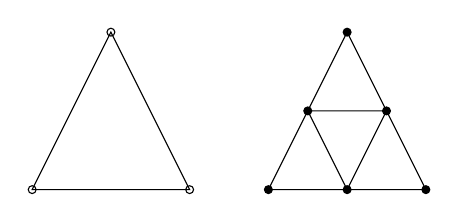
\begin{tikzpicture}
        % ������
        \draw (2, 1) -- (4, 1) -- (3, 3) -- cycle;
        % ��������
        \draw (2, 1) circle(0.05cm);
        \draw (4, 1) circle(0.05cm);
        \draw (3, 3) circle(0.05cm);
        % �ĸ�������
        \draw (5, 1) -- (6, 3) -- (7, 1) -- cycle;
        \draw (5.5, 2) -- (6.5, 2) -- (6, 1) -- cycle;
        % ��������
        \draw [fill = black] (5, 1) circle(0.05cm);
        \draw [fill = black] (6, 3) circle(0.05cm);
        \draw [fill = black] (7, 1) circle(0.05cm);
        \draw [fill = black] (5.5, 2) circle(0.05cm);
        \draw [fill = black] (6.5, 2) circle(0.05cm);
        \draw [fill = black] (6, 1) circle(0.05cm);
      \end{tikzpicture}
      \caption{��: ѹ�� $p$ ��Ԫ, $\circ$ Ϊ$p$��Ԫ�ϵ����ɶ�;
               ��: 4���ٶ�$v$ ��Ԫ, $\bullet$ ��ʾ$v$��Ԫ�ϵ����ɶ�.}
      \label{fig::p-v}
    \end{figure}

\section{�����Ŵ����ṹ}
    ����һ���У������ᵽ�ٶȵ�Ԫ��ѹ����Ԫ֮�������������������Ľ���������\cite{li2005multi}
    �еļ����Ŵ����ṹ���������ṹ��������h-����Ӧ���������Ǿͽ���һ���������ṹ��

    ��h-����Ӧ�У����������һ���������(����һ���ᵽ���ٶ�$u$��ѹ��$p$)���п����ڲ�ͬ�ĵط��������죬
    �����Ҫ�ֱ���������������ɢ��ֵ�⡣��ƴװ$\int_{\Omega} \nabla \cdot \vec{u} p$��һ��ʱ����Ϊ$\vec{u}$
    ��$p$�ڲ�ͬ�������ϣ������Ҫ������������֮�����ϵ���������������ڼ���������˵����С�������������죬
    �õ�������Ҫ�����������ֵĵط�����dz����С��ر�أ������С������Ԫ����������Ԫ�������ϰٱ���
    ��ʱ������������֮���Ӧ�Ĵ����Ƿdz�����ġ�Ϊ�˴�����Ч�Ķ���������Ӧ���ԣ�\cite{li2005multi}��ѡȡ
    �˼����Ŵ����������Ŵ��Ե�����ṹ��������Ϊ�㡢�ߡ��桢�塣��������޽ṹ���񣬼���Ҳ��ͨ������������ܵġ�
    ���ֲַ�����ݽṹ�����ṩ�򵥵ı�̷����Ϳ��ٵ���������㷨���Լ����������������

    �����Զ�ά����$\Omega$�ϵ�һ�������ʷ�$\mathcal{T}_0$Ϊ����������һ�¼����Ŵ����ṹ��Ϊ������Ԫ�ռ�ĵ�Ԫ
    ���ֿ����������ʷ��еĵ�ԪΪ���ε�Ԫ��$\tau$Ϊ$\mathcal{T}_0$�ļ��ε�Ԫ�������ʷ������м������ʶ������ڵ�
    ��ϵ�������һ������һ�������������е�һ�������������������������Ρ�ͬ���ģ����һ������һ������������
    �е�һ���������������������ߡ������ʷ��е�һ�������ο��Ա����ܳ��ĸ�С�������Ρ��������μ��ܵĹ����У���
    ���߷ֱ𱻷ֳ��������֡��������ʷ������е������ζ�����һ�Σ����ǿ��Եõ�һ�����ܵ������ʷ�$\mathcal{T}_1$,
    �����$\mathcal{T}_0$��һ��ȫ�ּ��ܡ�������μ��ܣ����ǿ��Եõ�һϵ�е������ʷ�$\{ \mathcal{T}_n\}$�� ���
    $\mathcal{T}_n$�е�һ��������$\tau_1$λ��$\mathcal{T}_{n-1}$�е�������$\tau_0$�У���$\tau_1$��������$\tau_0$
    ��һ�����ӡ����Ǹ�$\mathcal{T}_0$�е�����������һ������ĸ��ף������д�$\mathcal{T}_0$����������������������
    �IJ��������һ���������ݽṹ����ͼ\ref{fig::hgrometrytree}��ʾ�������Ҳ����Ϊ�����Ŵ�����
    \begin{figure}[h]
        \begin{minipage}[t]{0.4\textwidth}
          \centering
          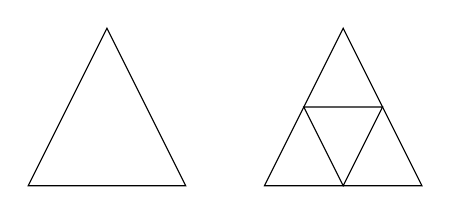
\begin{tikzpicture}
            % ������
            \draw (2, 1) -- (4, 1) -- (3, 3) -- cycle;
            \draw (5, 1) -- (6, 3) -- (7, 1) -- cycle;
            \draw (5.5, 2) -- (6.5, 2) -- (6, 1) -- cycle;
          \end{tikzpicture}
          \caption{ȫ�ּ���һ�ε�����}
        \end{minipage}
        \begin{minipage}[t]{0.6\textwidth}
          \centering
          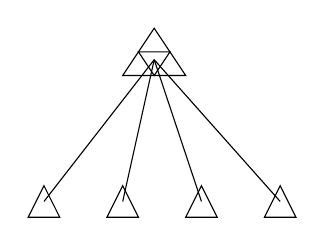
\begin{tikzpicture}
            %���������
            \draw (1.0, 0.0) -- (1.2, 0.4) -- (1.4, 0.0) -- cycle;
            \draw (2.0, 0.0) -- (2.2, 0.4) -- (2.4, 0.0) -- cycle;
            \draw (3.0, 0.0) -- (3.2, 0.4) -- (3.4, 0.0) -- cycle;
            \draw (4.0, 0.0) -- (4.2, 0.4) -- (4.4, 0.0) -- cycle;
            \draw (2.6, 2.4) -- (2.2, 1.8) -- (3.0, 1.8) -- cycle;
            \draw (2.4, 2.1) -- (2.6, 1.8) -- (2.8, 2.1) -- cycle;
            %������
            \draw (2.6, 2.0) -- (1.2, 0.2);
            \draw (2.6, 2.0) -- (2.2, 0.2);
            \draw (2.6, 2.0) -- (3.2, 0.2);
            \draw (2.6, 2.0) -- (4.2, 0.2);
          \end{tikzpicture}
          \caption{���ļ����Ŵ���}
        \end{minipage}
      \caption{�����Ŵ����ṹ}
      \label{fig::hgrometrytree}
    \end{figure}
    �ü����Ŵ����ṹ������h-����Ӧ�����ݾͲ�����ϸ�����ˡ�

\section{�ƶ����񷽷�}
    �ƶ����񷽷�����������ֵ�����У�Ѱ�Һõ�����(�����������й�)������
    �����Ͻ�����ֵ��⣬ʹ���ڲ��������ɶȵ�ǰ���£������ܵ���߼��㾫
    �ȡ��ƶ����񷽷�����������ƶ����ԣ��Լ��ڷ����������ϵ���ֵ�����
    ������\cite{budd2009adaptivity}��\cite{huang2011book}��\cite{tang2007book}
    ��ϵͳ�ظ������ƶ����񷽷��Ľ��ܡ��ƶ�����IJ����ǻ��ڵȷֲ�ԭ��
    (Equi-distribute Principle)������de Boor��1974��\cite{boor1974goodII}
    ����ġ��ȷֲ�ԭ���Ǹ���һ���ܷ�ӳ�ֲ��������������ָ�꣬������
    �ƶ�����ڵ�ʹ�����ָ���������Ͼ��ȷֲ�������ڼ��������Ƚϴ��
    �ط������У�����ʹ�����ֲ��ıȽϾ��ȣ��Ӷ���߼��㾫�ȡ�

    һЩ���ŵĶ������£���$\Omega \subset \mathbb{R}^N, N = 1, 2, 3$����
    ��������$\vec{x}$�������������ϵ����ꡣͬ���أ�$\Omega_c \subset
    \mathbb{R}^N$��ʾ�߼�����(��Ƽ�������)��$\vec{\xi}$Ϊ�����ꡣ

        de Boor ������һά���ε�֤�������£�

    ����$\Omega = [a, b]$,$\Omega_c = [0, 1]$�ֱ�Ϊ��������ͼ�������
    ��$\Omega_c$����һ����������$\{\xi_j = \frac{j}{N}| j = 0, 1, \cdots, N\}$,



\section{Ԥ��������}





\begin{theorem}
\label{th:MatrixNMCon} ��~$\MCR_1$~��~$(\ref{set:R_NM})$~����,
��~$\widehat{\MCR}_1$~ ��~$(\ref{set:R_hat_NM})$~���塣 �������~$A
\in \CS^{n \times n}$~����������ֵ������~$\MCR_1$~
������������ֵ���ǰ뵥��, ��ô��~$X_0 =
\I$~Ϊ��ʼ���~Newton~��~$(\ref{it:NM})$~�����������ľ�������~$\{X_k\}$~������
����~$A$~����~$p$~�θ�~$A^{1/p}$���ر��,
���~$A$~����������ֵ������~$\widehat{\MCR}_1\backslash\{0\}$,
��ô~Newton~��~$(\ref{it:NM})$~�Ƕ��������ġ�
\end{theorem}


\begin{figure}[h!]
\centering
\subfigure[]{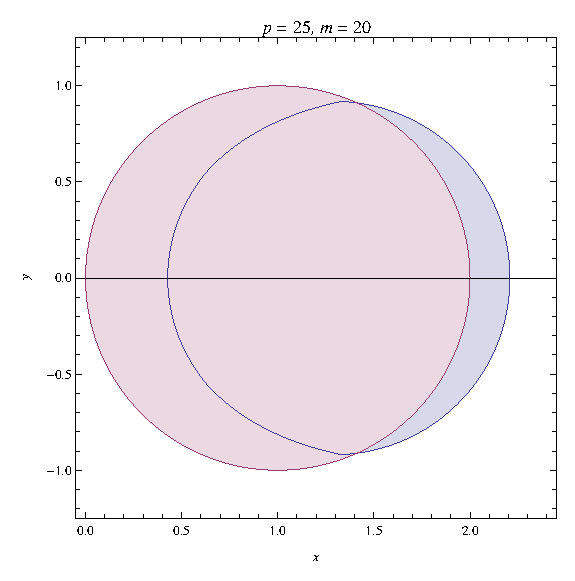
\includegraphics[width=0.3\textwidth]{fig_NM_ConvReg_p25m20.eps}}
\subfigure[]{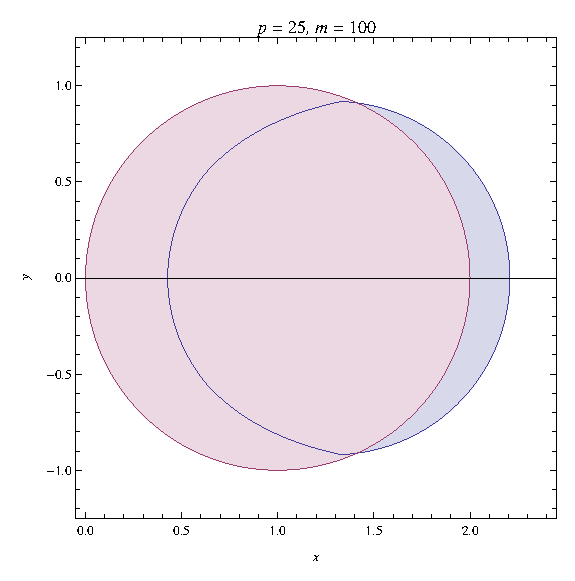
\includegraphics[width=0.3\textwidth]{fig_NM_ConvReg_p25m100.eps}}
\subfigure[]{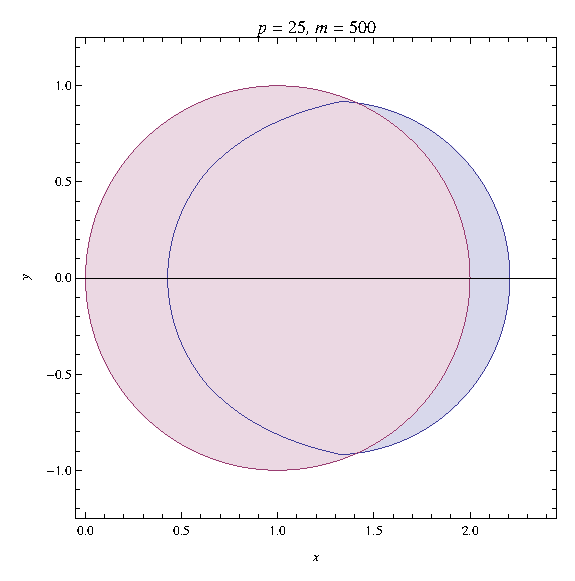
\includegraphics[width=0.3\textwidth]{fig_NM_ConvReg_p25m500.eps}}\\
\subfigure[]{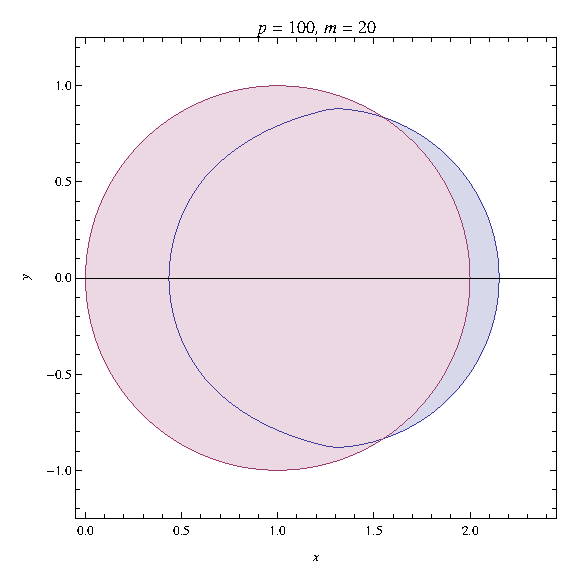
\includegraphics[width=0.3\textwidth]{fig_NM_ConvReg_p100m20.eps}}
\subfigure[]{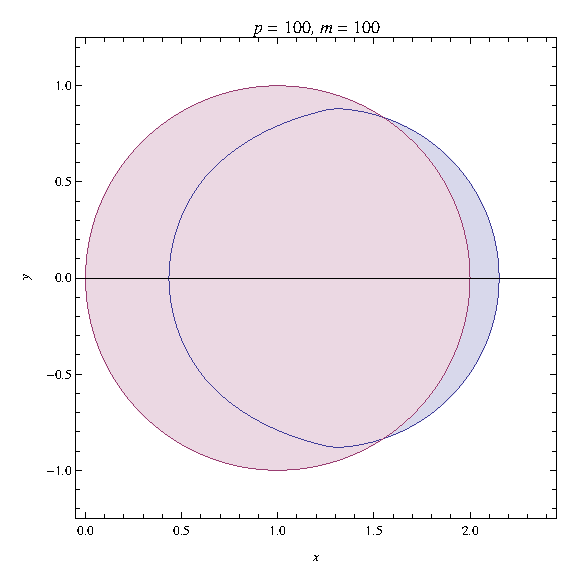
\includegraphics[width=0.3\textwidth]{fig_NM_ConvReg_p100m100.eps}}
\subfigure[]{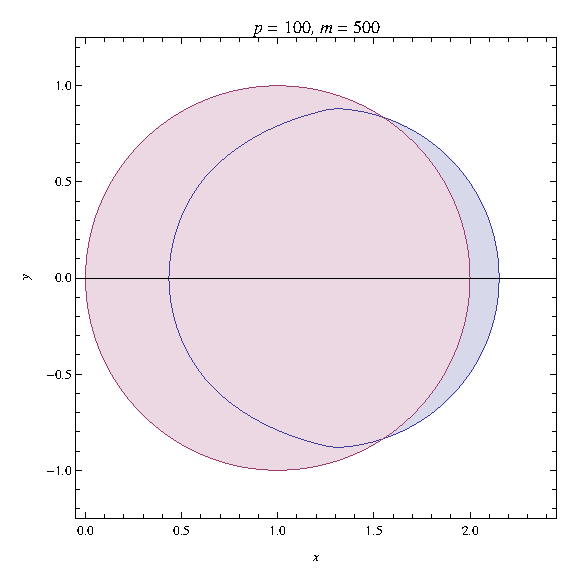
\includegraphics[width=0.3\textwidth]{fig_NM_ConvReg_p100m500.eps}}\\
\subfigure[]{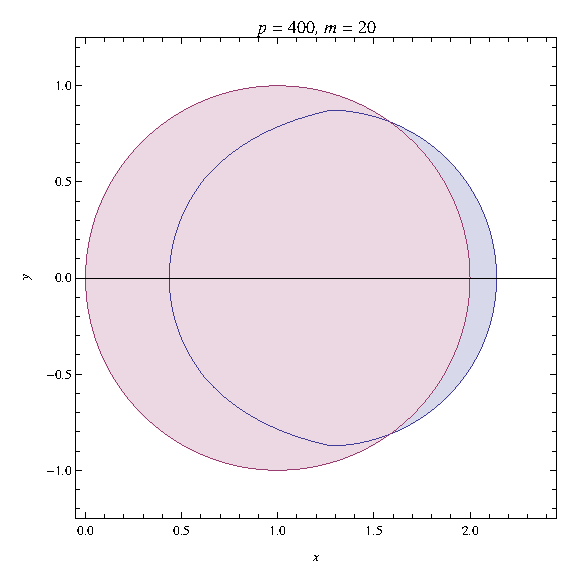
\includegraphics[width=0.3\textwidth]{fig_NM_ConvReg_p400m20.eps}}
\subfigure[]{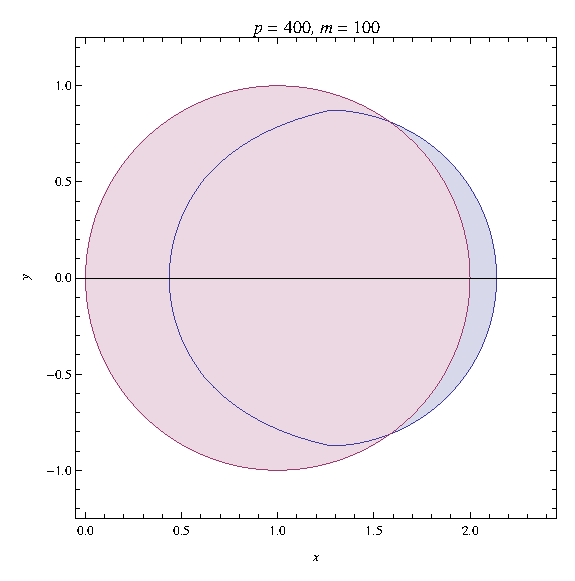
\includegraphics[width=0.3\textwidth]{fig_NM_ConvReg_p400m100.eps}}
\subfigure[]{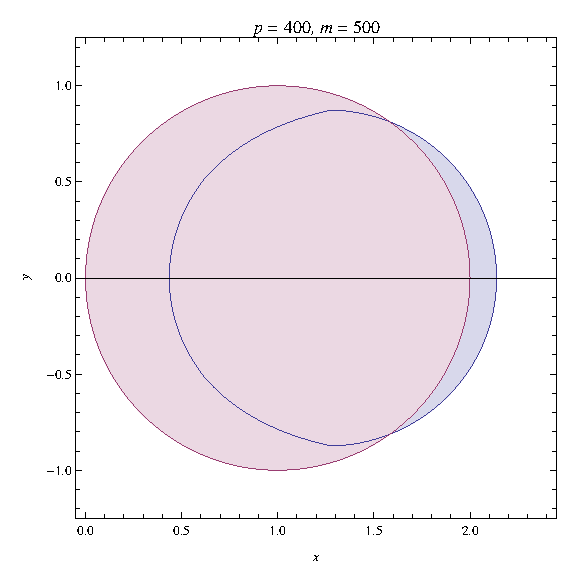
\includegraphics[width=0.3\textwidth]{fig_NM_ConvReg_p400m500.eps}}\\
%\caption{The approximating regions of $\MCR_1$ defined in
%(\ref{set:R_NM}) for $p = 25, 100, 400$ and $m = 20, 100, 500$,
%where the red and blue regions denote the sets $\{z\in\CS: 1-z \in
%\overline{\MCD}_1\}$ and $\{z\in \CS: 1-z \in \MCD_{0,1} \bigcap
%\MCD_{2,1}\}$, respectively. }
\caption{��~(\ref{set:R_NM})~������~$\MCR_1$~�ھ��ֲ�ͬ����~($p$~�ֱ�ȡ~25,
100, 400~��~$m$~�ֱ�ȡ~20, 100, 500)~�µĽ�����,
���к�ɫ���ʾ����~$\{z\in\CS: 1-z \in \overline{\MCD}_1\}$},
����ɫ���ʾ����~$\{z\in \CS: 1-z \in \MCD_{0,1}
\bigcap\MCD_{2,1}\}.$\label{fig:NM_ConvReg}
\end{figure}




\section{Ԥ������}

��֤������~\ref{th:MatrixNMCon}~ǰ, ��ҪһЩ���õ�Ԥ������.

��������һ������~$\lambda \in \CS$, ��

%For a complex number $\lambda \in \CS$, let
\begin{equation}
\label{fun:f(z)} f(z) := z^p - \lambda, \ \ \ z \in \CS
\end{equation}
��
\begin{equation}
\label{fun:r(z)} r(z,\lambda) := 1 - \lambda z^{-p}, \ \ \ z \in
\CS\backslash\{0\}.
\end{equation}

\begin{lemma}
\label{lem:NM_r(N(z))_r(z)} ��~$r(z,\lambda)$~��~$(\ref{fun:r(z)})$~
����. ����ij������~$z \in \CS\backslash\{0\}$, ��~$r(z,\lambda) \in
\mathcal {D}_{0,1}\backslash\{1\}$,
����~$\MCD_{0,1}$~��~$(\ref{set:D0_NM})$~����,
����~$(\ref{it:NM_fun})$~�ı�����ʽ���õ���~$N(z)$~�ж�����
\begin{equation}
\label{eq:r(N(z))_1} r(N(z),\lambda) = \phi_1(r(z,\lambda)),
\end{equation}
����~$\phi_1(z)$~��~$(\ref{fun:phi(z)_NM})$~����. ����,
�����µĹ���: ��~$r(z,\lambda) \in
\overline{\MCD}_1\backslash\{0,1\}$~ʱ,
\begin{equation}
\label{ineq:abs_r(N(z))_1} |r(N(z),\lambda)| < |r(z,\lambda)|^2.
\end{equation}
��~$r(z,\lambda) \in \mathcal {D}_{0,1}\backslash\{1\}$~ʱ,
\begin{equation}
\label{ineq:abs_r(N(z))_2} |r(N(z),\lambda)| \leq \sup_{m \geq
2}\left\{\left|\frac{S_{1,m}(u)}{u^2}\right|\right\}\cdot \frac{|u|
+ |r(z,\lambda)|}{|u| - |r(z,\lambda)|} \cdot |r(z,\lambda)|^2,
\end{equation}
����~$\overline{\MCD}_1$~Ϊ~$\MCD_1$~�ıհ�,
��~$\MCD_1$~��~$(\ref{set:D1_NM})$~����,
$S_{1,m}(u)$~��~$(\ref{ser:Sm(z)_NM})$~�����Ҷ���ÿһ��~$u \in
\MCD_{0,1}$~������~$|u| > |r(z,\lambda)|$, $m \geq 2$.
\end{lemma}


\begin{proof}

%For any $z \in \CS\backslash\{0\}$, $N(z)$ exists by
%(\ref{it:NM_fun}). Note that

��������ĸ���~$z \in \CS\backslash\{0\}$,
��~(\ref{it:NM_fun})~֪~$N(z)$~�Ǵ��ڵ�. ����

\begin{equation}
\label{eq:N(z)} N(z) = \frac{1}{p}z\left[(p-1)+\lambda z^{-p}\right]
= z\left[1+\frac{1}{p}r(z,\lambda)\right] \neq 0.
\end{equation}
%It follows that
��
\begin{equation}
\label{eq:r(N(z))} r(N(z),\lambda) =
1-\left[1+\frac{1}{p}r(z,\lambda)\right]^{-p}(1-r(z,\lambda)) =
\phi_1(r(z,\lambda)),
\end{equation}
%which shows (\ref{eq:r(N(z))_1}) holds.
����~(\ref{eq:r(N(z))_1})~�dz�����.

%If $r(z,\lambda) \in \overline{\MCD}_1\backslash\{0,1\} \subset
%\MCD_{0,1}$, then, by (\ref{fun:phi1(z)_series}) and
%(\ref{eq:r(N(z))}), one has that

��~$r(z,\lambda) \in \overline{\MCD}_1\backslash\{0,1\} \subset
\MCD_{0,1}$, ����~(\ref{fun:phi1(z)_series})~��~(\ref{eq:r(N(z))}),
��ע�⵽���������~$w \in \overline{\MCD}_1\backslash\{1\}$,
����ʽ~$|c_3 + c_4 w| < c_3 + c_4$~���dz�����, ���ǿɵ�
\begin{align}
|r(N(z),\lambda)|  & = |\phi(r(z,\lambda))| \nonumber\\
& = |r(z,\lambda)|^2 \left| \sum_{j =
2}^\infty c_{1,j} r^{j-2}(z,\lambda) \right| \nonumber\\
& \leq |r(z,\lambda)|^2 \left[|c_{1,3} + c_{1,4} r(z,\lambda)| +
\sum_{j = 4}^\infty c_{1,j} |r(z,\lambda)|^{j-2}
\right] \nonumber\\
& < |r(z,\lambda)|^2 \sum_{j = 2}^\infty c_{1,j} =
|r(z,\lambda)|^2\nonumber\\
& \leq |r(z,\lambda)|. \label{ineq:abs_r(N(z))}
\end{align}
%from the fact that $|c_3 + c_4 w| < c_3 + c_4$ for all $w \in
%\overline{\MCD}_1\backslash\{1\}$. Thus, (\ref{ineq:abs_r(N(z))_1})
%is proved.
��~(\ref{ineq:abs_r(N(z))_1})~�dz�����.


%If $r(z,\lambda) \in \mathcal {D}_0\backslash\{1\}$, based on
%(\ref{fun:phi1(z)_series}) and (\ref{eq:r(N(z))}) again, we have

��~$r(z,\lambda) \in \mathcal {D}_0\backslash\{1\}$,
����~(\ref{fun:phi1(z)_series})~��~(\ref{eq:r(N(z))})~��֪,
��������� ~$u \in \CS\backslash\{0\}$~��
\begin{align*}
r(N(z),\lambda) &  = \phi_1(r(z,\lambda))\\
& = \sum_{j=2}^\infty c_{1,j} r^j(z,\lambda)\\
& = \left[\sum_{j=2}^\infty c_{1,j} u^{j-2}
\left(\frac{r(z,\lambda)}{u}\right)^{j-2}\right] \cdot
r^2(z,\lambda).
\end{align*}
%holds for any $u \in \CS\backslash\{0\}$. Since, for any $m \geq 2$,
���������~$m \geq 2$, Ӧ��~Abel~�任�ɵ�
\begin{align*}
\sum_{j=2}^m c_{1,j} u^{j-2}
\left(\frac{r(z,\lambda)}{u}\right)^{j-2} & = \sum_{j=2}^{m-1}
\left(\sum_{\ell=2}^j c_{1,\ell} u^{\ell-2}\right)\left(1 -
\frac{r(z,\lambda)}{u}\right)\left(\frac{r(z,\lambda)}{u}\right)^{j-2}\\
& \ \ \ + \left(\sum_{\ell = 2}^m c_{1,\ell} u^{\ell-2}\right)\cdot
\left(\frac{r(z,\lambda)}{u}\right)^{m-2}.
\end{align*}
%by Abel transformation, we have
����
\begin{align*}
\left|\sum_{j=2}^m c_{1,j} u^{j-2}
\left(\frac{r(z,\lambda)}{u}\right)^{j-2}\right| & \leq \sup_{2\leq
j \leq m-1} \left\{\left|\sum_{\ell=2}^j c_{1,\ell}
u^{\ell-2}\right|\right\} \cdot \left|1 -
\frac{r(z,\lambda)}{u}\right| \cdot \sum_{j=2}^{m-1}
\left|\frac{r(z,\lambda)}{u}\right|^{j-2}\\
& \ \ \ + \left|\frac{S_{1,m}(u)}{u^2} \right|\cdot
\left|\frac{r(z,\lambda)}{u}\right|^{m-2}, \quad m >2.
\end{align*}
%Then, letting $m \to \infty$ in the above inequality, it follows
%that
����������ʽ����~$m \to \infty$, ����������~$r(z,\lambda) \in
\mathcal {D}_0\backslash\{1\}$~�������ϵ~$|u|
> |r(z,\lambda)|$~�����⸴��~$u
\in \mathcal {D}_0$, ��
\begin{align*}
|r(E(z),\lambda)|  & \leq \sup_{m \geq 2} \left\{\left|\sum_{j=2}^m
c_{1,j} u^{j-2}\right|\right\} \cdot \left|1 -
\frac{r(z,\lambda)}{u}\right| \cdot
\sum_{m=2}^\infty \left|\frac{r(z,\lambda)}{u}\right|^{m-2}\cdot |r(z,\lambda)|^2 \\
& = \sup_{m \geq 2}
\left\{\left|\frac{S_{1,m}(u)}{u^2}\right|\right\} \cdot
\frac{\left|1 - \frac{r(z,\lambda)}{u}\right|}{1 -
\left|\frac{r(z,\lambda)}{u}\right|} \cdot |r(z,\lambda)|^2 \\
& = \sup_{m \geq 2}
\left\{\left|\frac{S_{1,m}(u)}{u^2}\right|\right\} \cdot \frac{|u| +
|r(z,\lambda)|}{|u| - \left|r(z,\lambda)\right|} \cdot
|r(z,\lambda)|^2.
\end{align*}
%for any $r(z,\lambda) \in \mathcal {D}_0\backslash\{1\}$ and any $u
%\in \mathcal {D}_0$ subject to $|u|
%> |r(z,\lambda)|$, which verifies (\ref{ineq:abs_r(N(z))_2}). The
%proof is completed.
�Ӷ�~(\ref{ineq:abs_r(N(z))_2})~��֤. ֤��.
\end{proof}



\begin{lemma}
\label{lem:NM_r(z)_convergence1} %Let $r(z,\lambda)$ be defined in
%$(\ref{fun:r(z)})$. If $r(z_0,\lambda) \in
%\overline{\MCD}_1\backslash\{0,1\}$ for some $z_0 \in
%\CS\backslash\{0\}$, then the sequence $\{z_k\}$ starting from $z_0$
%generated by the scalar case of $(\ref{it:NM})$ for solving
%$(\ref{fun:f(z)})$ exists,

��~$r(z,\lambda)$~��~$(\ref{fun:r(z)})$~����. ����ij������~$z_0 \in
\CS\backslash\{0\}$, ��~$r(z_0,\lambda) \in
\overline{\MCD}_1\backslash\{0,1\}$,
����~$(\ref{it:NM})$~�ı�����ʽ~$($��~$z_0$~Ϊ��ʼ��$)$~��������������~$\{z_k\}$~
���ж����, ���й���ʽ:
\begin{equation}
\label{ineq:NM_abs_r(zk)_1} |r(z_k,\lambda)| \leq
q_1^{2^{k-1}}(z_0), \ \ \ k = 1, 2, \ldots,
\end{equation}
%where
����
\begin{equation}
\label{cons:NM_q1(z0)} q_1(z_0) = q_1(z_0,\lambda) :=
\left|\sum_{j=2}^\infty c_{1,j} r^{j-1}(z_0,\lambda)\right| < 1.
\end{equation}
%and so $|r(z_k,\lambda)| \to 0$ with order $2$ as $k \to \infty$.
�ɴ˿�֪, ��~$k \to \infty$~ʱ~$|r(z_k,\lambda)|$~������~0,
�������ٶ��Ƕ��׵�.
\end{lemma}

\begin{proof}
%For $z_0$ chosen, $q_1(z_0) < 1$ follows from the same arguments
%used in (\ref{ineq:abs_r(N(z))}). By (\ref{ineq:abs_r(N(z))_1}) in
%Lemma \ref{lem:NM_r(N(z))_r(z)}, $z_1 = E(z_0)$ exists and

���ڸ�����~$z_0$,
������~(\ref{ineq:abs_r(N(z))})~�Ĵ�����ʽ��֪~$q_1(z_0) < 1$.
��������~\ref{lem:NM_r(N(z))_r(z)}~�е�~(\ref{ineq:abs_r(N(z))_1})~֪~$z_1
= E(z_0)$~�Ǵ��ڵIJ�����
$$
|r(z_1,\lambda)| = q_1(z_0)|r(z_0,\lambda)| \leq q_1(z_0) < 1.
$$
%Suppose that $z_k$ exists and (\ref{ineq:NM_abs_r(zk)_1}) holds for
%some $k \geq 1$, then by Lemma \ref{lem:NM_r(N(z))_r(z)} again,
%$z_{k+1} = E(z_k)$ exists and
����ijһ~$k \geq 1$,
����~$z_k$~�Ǵ��ڵ���~(\ref{ineq:NM_abs_r(zk)_1})~�dz�����,
��������~\ref{lem:NM_r(N(z))_r(z)}~��֪~$z_{k+1} =
E(z_k)$~�Ǵ��ڵIJ�����
\begin{equation*}
|r(z_{k+1},\lambda)| < |r(z_{k},\lambda)|^2  \leq
\left[q_1^{2^{k-1}}(z_0)\right]^2 = q_1^{2^{k}}(z_0).
\end{equation*}
%Thus, (\ref{ineq:NM_abs_r(zk)_1}) holds for $k+1$. By induction,
%$\{z_k\}$ exists and (\ref{ineq:NM_abs_r(zk)_1}) holds. Furthermore,
%$r(z_k,\lambda) \to 0$ with order 2 as $k \to \infty$, which
%completes the proof.
�ɴ�֪, (\ref{ineq:NM_abs_r(zk)_1})~����~$k+1$~��������Ȼ����.
�����ɹ��ɷ�֪,
����~$\{z_k\}$~�Ǵ��ڵ���~(\ref{ineq:NM_abs_r(zk)_1})~�����. ֤��.
\end{proof}



%The following lemma says that, besides in $
%\overline{\MCD}_1\backslash\{0,1\}$, it also guarantees
%$r(z_k,\lambda)$ converges quadratically to 0 as $k \to \infty$ when
%$r(z_0,\lambda) \in \MCD_{2,1} \bigcap \MCD_{0,1}\backslash\{1\}$
%for some $z_0 \in \CS\backslash\{0\}$.

����ij������~$z_0 \in \CS\backslash\{0\}$,
����~\ref{lem:NM_r(z)_convergence1}~ ˵����~$r(z_0,\lambda) \in
\overline{\MCD}_1\backslash\{0,1\}$~ʱ�ɱ�֤~$r(z_k,\lambda)$~�Ƕ���������~0,
�������������, ����֮��, ��~$r(z_0,\lambda) \in \MCD_{2,1} \bigcap
\MCD_{0,1}\backslash\{1\}$~ʱ,
��Ȼ���Ա�֤~$r(z_k,\lambda)$~�Ƕ���������~0.

\begin{lemma}
\label{lem:NM_r(z)_convergence2}  %For any $z_0 \in
%\CS\backslash\{0\}$ satisfying $r(z_0,\lambda) \in \MCD_{2,1}
%\bigcap \MCD_{0,1}\backslash\{1\}$ and

��~$r(z,\lambda)$~��~$(\ref{fun:r(z)})$~����. ����ijһ����~$z_0 \in
\CS\backslash\{0\}$, ��~$r(z_0,\lambda) \in \MCD_{2,1} \bigcap
\MCD_{0,1}\backslash\{1\}$~��
\begin{equation}
\label{cons:NM_q2(z0)} q_2(z_0) = q_2(z_0,\lambda) := \sup_{m \geq
2} \left\{\frac{|S_{1,m}(r(z_0,\lambda))|}{|r(z_0,\lambda)|}\right\}
\cdot \frac{|r(z_0,\lambda)|
+|\phi_1(r(z_0,\lambda))|}{|r(z_0,\lambda)| -
|\phi_1(r(z_0,\lambda))|} < 1,
\end{equation}
%where $\MCD_{2,1}$ is defined in $(\ref{set:D2_NM})$, the sequence
%$\{z_k\}$ generated by the scalar form of $(\ref{it:NM})$ starting
%from $z_0$ for solving $(\ref{fun:f(z)})$ exists,
����~$\MCD_{2,1}$~��~$(\ref{set:D2_NM})$~����,
����~$(\ref{it:NM})$~�ı�����ʽ~$($��~$z_0$~Ϊ��ʼ��$)$~
��������������~$\{z_k\}$~���������,
�������¹���:
\begin{equation}
\label{ineq:NM_abs_r(zk)_2} |r(z_k,\lambda)| \leq q_2^{2^k-1}(z_0)
\cdot |r(z_0,\lambda)|, \quad k = 0, 1, \ldots.
\end{equation}
%and so $|r(z_k,\lambda)| \to 0$ with order $2$ as $k \to \infty$.
�ɴ˿�֪, ��~$k \to \infty$~ʱ~$|r(z_k,\lambda)|$~������~$0$,
�������ٶ��Ƕ��׵�.
\end{lemma}

\begin{proof}
%For $z_0$ chosen, we have $r(z_0,\lambda) \in \mathcal
%{D}_{0,1}\backslash\{1\}$. So, $z_1 = N(z_0)$ exists and $z_1 \neq
%0$ by (\ref{eq:N(z)}). Recall that $S_{1,m}(r(z_0,\lambda)) \to
%\phi_1(r(z_0,\lambda))$ as $k\to\infty$ implies
��Ȼ, ���ڸ�����~$z_0$~��~$r(z_0,\lambda) \in \mathcal
{D}_{0,1}\backslash\{1\}$. ��~$z_1 =
N(z_0)$~��������~(\ref{eq:N(z)})~֪~$z_1 \neq 0$. ע�⵽,
��~$k\to\infty$~ʱ~$S_{1,m}(r(z_0,\lambda)) \to
\phi_1(r(z_0,\lambda))$, ����~(\ref{cons:NM_q2(z0)})~�ɵ�
$$
\left|\frac{\phi_1(r(z_0,\lambda))}{r(z_0,\lambda)}\right| \leq
\sup_{m\geq2}
\left\{\left|\frac{S_{1,m}(r(z_0,\lambda))}{r(z_0,\lambda)}\right|\right\}
< q_2^2(z_0)<1,
$$
%by (\ref{cons:NM_q2(z0)}), we have
������
$$
|r(z_1,\lambda)| = |\phi_1(r(z_0,\lambda))| =
\left|\frac{\phi_1(r(z_0,\lambda))}{r(z_0,\lambda)}r(z_0,\lambda)\right|
< q_2^2(z_0)\cdot|r(z_0,\lambda)|,
$$
%and (\ref{ineq:NM_abs_r(zk)_2}) holds for $k=1$.  Assume $z_0, z_1,
%\ldots, z_k$ exist and satisfy (\ref{ineq:NM_abs_r(zk)_2}). Then
����~$k=1$~ʱ~(\ref{ineq:NM_abs_r(zk)_2})~�dz�����. �ּ���~$z_0,
z_1, \ldots, z_k$~���Ǵ��ڵ�������~(\ref{ineq:NM_abs_r(zk)_2}), ��
$$
|r(z_k,\lambda)| \leq q_2^2(z_0)|r(z_0,\lambda)|< |r(z_0,\lambda)| <
p.
$$
%So, by Lemma \ref{lem:NM_r(N(z))_r(z)} with $u = r(z_0,\lambda)$,
%$z_{k+1} = N(z_k)$ exists, $z_{k+1} \neq 0$ and
������~\ref{lem:NM_r(N(z))_r(z)}~ (ȡ~$u =
r(z_0,\lambda)$)~��֪~$z_{k+1} = N(z_k)$~�Ǵ��ڵ���~$z_{k+1} \neq
0$. ��һ����
\begin{align*}
|r(z_{k+1},\lambda)| & = |\phi(r(z_k,\lambda))| \\
& \leq \sup_{m \geq 2}
\left\{\frac{|S_{1,m}(r(z_0,\lambda))|}{|r(z_0,\lambda)|^2}\right\}\cdot
\frac{|r(z_0,\lambda)|
+|\phi_1(r(z_0,\lambda))|}{\Big||r(z_0,\lambda)| -
|\phi(r(z_0,\lambda))|\Big|} \cdot |r(z_k,\lambda)|^2 \\
& \leq \sup_{m \geq 2}
\left\{\frac{|S_{1,m}(r(z_0,\lambda))|}{|r(z_0,\lambda)|^2}\right\}\cdot
\frac{|r(z_0,\lambda)|
+|\phi_1(r(z_0,\lambda))|}{\Big||r(z_0,\lambda)| -
|\phi_1(r(z_0,\lambda))|\Big|}
\left[q_2^{2^k-1}(z_0)\right]^2\cdot|r(z_0,\lambda)|^2 \\
& = \sup_{m \geq 2}
\left\{\frac{|S_{1,m}(r(z_0,\lambda))|}{|r(z_0,\lambda)|}\right\}\cdot
\frac{|r(z_0,\lambda)|
+|\phi_1(r(z_0,\lambda))|}{\Big||r(z_0,\lambda)| -
|\phi_1(r(z_0,\lambda))|\Big|} \cdot [q_2(z_0)]^{2^{k+1}-2} \cdot
|r(z_0,\lambda)| \\
& = [q_2(z_0)]^{2^{k+1}-1} \cdot |r(z_0)|,
\end{align*}
%which shows (\ref{ineq:NM_abs_r(zk)_2}) by induction. The proof is
%completed.
�ɴ�, ���ݹ��ɷ�֪~(\ref{ineq:NM_abs_r(zk)_2})~��֤. ֤��.
\end{proof}




���IJ�.
��~$z(\lambda)$~��~$\Int(\MCR_{1,1})$~�ǽ�����������~$p$~�θ��ĵ�ֵ��֧��,
����������~$k\geq0$~����~$z_k(1) \equiv 1$, ��~$z(1) =
1$~��~$z(\lambda)$~���ڰ���~1~�ĵ�ֵ��֧��. ��������~$\lambda \in
\Int(\MCR_{1,1})$, $z(\lambda)$~��������~$p$~�θ�. ע�⵽,
�������~$\lambda_0 \in
\partial\MCR_{1,1}$, ��~$\lambda
\to \lambda_0 \ (\lambda \in \Int(\MCR_{1,1}))$~ʱ~$z(\lambda) \to
z(\lambda_0)$, �����֪~$z(\lambda_0)$~����~$\lambda_0 \in
\partial\MCR_{1,1}$~����~$p$~�θ�.




ͬ���ɵڶ���֪, �������~$\lambda \in \MCR_{1,2}$,
$z(\lambda)$~�ǽ�����������~$p$~�θ������ĵ�ֵ��֧��. ����,
��������֤��~$\MCR_{1,2}$~����~$\partial\MCR_{1,1}$~ijһ����,
��ô��֪, ��~$\lambda \in
\MCR_{1,2}$~ʱ��~$z(\lambda)$~�ĵ�ֵ��֧�뵱~$\lambda \in
\MCR_{1,1}$~ʱ��~$z(\lambda)$~�ĵ�ֵ��֧��һ����. �Ӷ��ɵ�,
������~$\lambda \in \MCR_{1,1} \bigcup\MCR_{1,2}$,
��~$z(\lambda)$~Ϊ����~$p$~�θ�. ���,
����ֻ��֤��~$\MCR_{1,2}$~������~$\partial\MCR_{1,1}$~��ijһ���ּ���.



���ڷֱ���~(\ref{set:R11})~��~(\ref{set:R12})~�����~$\MCR_{1,1}$~��
~$\MCR_{1,2}$, ��ȡ~$z_0 \equiv 1$, ����~$\MCR = \MCR_{1,1} \bigcup
\MCR_{1,2}$. ����, ������~\ref{lem:ScalarNMCon1}~�������õ���������:


\begin{corollary}
\label{cor:NM_zk_convergence1} %For any $\lambda \in \MCR_1$ defined
%in $(\ref{set:R_NM})$, the sequence $\{z_k(\lambda)\}$ generated by
%scalar Newton iteration $(\ref{it:NM})$ with $z_0 = 1$ for solving
%$(\ref{fun:f(z)})$ converges to the principal $p$th root
%$\lambda^{1/p}$. Moreover, if $\lambda \neq 0$, then the convergence
%order is $2$.
%
���������~$\lambda \in \MCR_1$,
����~$\MCR_1$~��~$(\ref{set:R_NM})$~����, �ɱ���
~Newton~��~$(\ref{it:NM})$~��~$z_0 =
1$~Ϊ��ʼ����е�������������~$\{z_k(\lambda)\}$~
������~$\lambda$~����~$p$~�θ�~$\lambda^{1/p}$. ��һ��, ��~$\lambda
\neq 0$, ���������ٶ��Ƕ��׵�.
\end{corollary}





%Next, we consider the case of matrix form. For the matrix $A \in
%\CS^{n \times n}$ defined in (\ref{eq:f(X)=0}), let

�������ǿ��Ǿ��������. ������~(\ref{eq:f(X)=0})~�����ľ���~$A \in
\CS^{n \times n}$, ��
\begin{equation}
\label{fun:NM_R(X)} R(X) := \I - A X^{-p}, \ \ \ p \geq 2,
\end{equation}
%for any nonsingular matrix $ X \in \CS^{n \times n}$.
����~$ X \in \CS^{n \times n}$~�Ƿ������.

\begin{lemma}
\label{lem:R(N(X))_R(X)} %Let $X \in \CS^{n\times n}$ be a
%nonsingular matrix commuting with $A$ and $R(X)$ be defined in
%$(\ref{fun:NM_R(X)})$. If the spectrum $\sigma(R(X)) \subset
%\MCD_{0,1}$ for some nonsingular matrix $X \in \CS^{n \times n}$,
%where $\MCD_{0,1}$ is defined in $(\ref{set:D0_NM})$, then $N(X)$
%generated by $(\ref{it:NM_fun})$ is nonsingular, commutes with $A$
%and
%
�����~$X \in \CS^{n\times n}$~�Ƿ����������~$A$~�ǿɽ�����,
$R(X)$~��~$(\ref{fun:NM_R(X)})$~����.
���~$R(X)$~��������~$\sigma(R(X)) \subset \MCD_{0,1}$,
����~$\MCD_{0,1}$~��~$(\ref{set:D0_NM})$~����,
��ô��~$(\ref{it:NM_fun})$~����~$N(X)$~�Ƿ������,
��~$A$~�ǿɽ�����������
\begin{equation}
\label{eq:R(N(X))} R(N(X)) = \I - \left[\I - \frac{1}{p}
R(X)\right]^{-p}\cdot(\I - R(X)) = \phi_1(R(X)),
\end{equation}
%where $\phi_1$ is defined in $(\ref{fun:phi(z)_NM})$.
%
����~$\phi_1$~��~$(\ref{fun:phi(z)_NM})$~����.
\end{lemma}

\begin{proof}
%Clearly, $N(X)$ given by (\ref{it:NM_fun}) exists for any
%nonsingular matrix $X \in \CS^{n \times n}$. Since $\sigma(R(X))
%\subset \MCD_{0,1}\backslash\{0\}$, we get $ \I - \frac{1}{p} R(X)$
%is nonsingular by Neumann Lemma. It follows that

��Ȼ, ��~$X \in \CS^{n \times n}$~�Ƿ��������,
����~(\ref{it:NM_fun})~�����~$N(X)$~�Ǵ��ڵ�. ����~$\sigma(R(X))
\subset \MCD_{0,1}\backslash\{0\}$, ����~Neumann~������֪����
$$
\I - \frac{1}{p} R(X)
$$
�Ƿ������. �����ɵ�ʽ
\begin{align*}
N(X) = \frac{1}{p} X \left[(p - 1)\I + AX^{-p}\right]
 = X \left[\I - \frac{1}{p}R(X)\right]
\end{align*}
%is also nonsingular and commutes with $A$, and
%
֪����~$N(X)$~�Ƿ����������~$A$~�ǿɽ�����. �ɴ˿ɽ�һ���õ�
\begin{equation*}
R(N(X)) = \I - \left[\I - \frac{1}{p} R(X)\right]^{-p}\cdot(\I -
R(X)) = \phi_1(R(X))
\end{equation*}
%by the assumption of $X$ commutes with $A$. This completes the
%proof.
%
������һ����ʽ�Ǹ���~$X$~��~$A$~�ǿɽ����ļ���õ���. ֤��.
\end{proof}



%Thanks to Lemma \ref{lem:R(N(X))_R(X)}, we have

��������~\ref{lem:R(N(X))_R(X)}~��ֱ�ӵõ���������:

\begin{corollary}
\label{cor:N(Xk)} %If $X_0 \in \CS^{n \times n}$ commutes with $A$
%and the spectrum $\sigma(R(X_0)) \subset \MCD_{0,1}$, where
%$\MCD_{0,1}$ is defined in $(\ref{set:D0_NM})$, then the sequence
%$\{X_k\}$ starting from $X_0$ generated by Newton's method
%$(\ref{it:NM})$ for solving $(\ref{eq:f(X)=0})$ exists.
%
�������~$X_0 \in \CS^{n \times
n}$~��~$A$~�ǿɽ�������~$R(X_0)$~��������~$\sigma(R(X_0)) \subset
\MCD_{0,1}$, ����~$\MCD_{0,1}$~��~$(\ref{set:D0_NM})$~����,
��ô��~Newton~��~$(\ref{it:NM})$~��~$X_0$~Ϊ
��ʼ����е��������ľ�������~$\{X_k\}$~���ж����.
\end{corollary}



\begin{lemma}
\label{lem:norm_R(N(X))_R(X)} %If the spectrum $\sigma(R(X)) \subset
%\MCD_1\backslash\{0\}$ for some nonsingular matrix $X \in \CS^{n
%\times n}$, where $R(X)$  be defined in $(\ref{fun:NM_R(X)})$ and
%$\MCD_1$ is defined in $(\ref{set:D1_NM})$, then, there is a
%sub-multiplicative matrix norm $\|\cdot\|$ such that $\|R(X)\| \leq
%1$ and
%
��~$R(X)$~��~$(\ref{fun:NM_R(X)})$~����, $X \in \CS^{n \times
n}$~�Ƿ������. ���~$R(X)$~��������~$\sigma(R(X)) \subset
\MCD_1\backslash\{0\}$, ����~$\MCD_1$~��~$(\ref{set:D1_NM})$~����,
��ô����һ���οɼӵľ�����~$\|\cdot\|$~ʹ��~$\|R(X)\| \leq 1$~��
\begin{equation}
\label{ineq:NM_norm_R(E(X))_1} \|R(E(X))\| \leq
\frac{\phi_1(\|R(X)\|)}{\|R(X)\|^2} \cdot \|R(X)\|^2 < \|R(X)\|^2,
\end{equation}
%where $\phi_1$ is defined by $(\ref{fun:phi(z)_NM})$.
%
����~$\phi_1$~��~$(\ref{fun:phi(z)_NM})$~����.
\end{lemma}

\begin{proof}
%It follows from Lemma \ref{lem:R(N(X))_R(X)} that $R(N(X))$ exists.
%Since the spectrum $\sigma(R(X)) \subset \MCD_1$, the spectral
%radius of $R(X)$ is less than 1. So, there is a sub-multiplicative
%matrix norm $\|\cdot\|$ such that $\|R(X)\| < 1$. Note that, for any
%$u \in (0,1)$,  It follows from that
%
������~\ref{lem:R(N(X))_R(X)}~��֪~$R(N(X))$~�Ǵ��ڵ�.
��~$\sigma(R(X)) \subset \MCD_1$, ��~$R(X)$~���װ뾶С��~1.
�Ӷ�����һ���οɼӵľ�����~$\|\cdot\|$~ʹ��~$\|R(X)\| < 1$.
ע�⵽, ���������~$u \in (0,1)$~����
$$
\frac{\phi(u)}{u^2} = \sum_{j=2}^\infty c_{1,j} u^{j-2} <
\sum_{j=2}^\infty c_{1,j} = 1.
$$
%Thus, this together with (\ref{eq:R(N(X))}) gives that
%
����, ���~(\ref{eq:R(N(X))})~�ɵ�
\begin{align*}
\|R(N(X))\| = \|\phi_1(R(X))\| & \leq \phi_1(\|R(X)\|) \\
& = \frac{\phi_1(\|R(X)\|)}{\|R(X)\|^2}\|R(X)\|^2 \\
& < \|R(X)\|^2,
\end{align*}
%which shows (\ref{ineq:NM_norm_R(E(X))_1}). The proof is completed.
%
���~(\ref{ineq:NM_norm_R(E(X))_1})~�dz�����. ֤��.
\end{proof}



\begin{lemma}
\label{lem:NM_R(X)_convergence1} %Let $R(X)$  be defined in
%$(\ref{fun:NM_R(X)})$. Suppose the spectrum $\sigma(R(X_0)) \subset
%\mathcal {D}_1\backslash\{0\}$ for some nonsingular matrix $X_0 \in
%\CS^{n \times n}$ and that $\|R(X_0)\| < 1$ for a sub-multiplicative
%matrix norm $\|\cdot\|$, where $\mathcal {D}_1$ is defined in
%$(\ref{set:D1_NM})$. Let $\{X_k\}$ be the sequence starting from
%$X_0$ generated by Newton's method $(\ref{it:NM})$ for solving
%$(\ref{eq:f(X)=0})$. Then we have
%
��~$R(X)$~��~$(\ref{fun:NM_R(X)})$~����, ����~$X_0 \in \CS^{n \times
n}$~�Ƿ������. ��~$R(X_0)$~��������~$\sigma(R(X_0)) \subset
\mathcal
{D}_1\backslash\{0\}$~�Ҵ���һ���οɼ��Եľ�����~$\|\cdot\|$~ʹ��~$\|R(X_0)\|
< 1$, ����~$\mathcal {D}_1$~��~$(\ref{set:D1_NM})$~����.
��~$\{X_k\}$~����~Newton~��~$(\ref{it:NM})$~��~$X_0$~Ϊ��ʼ����е��������ľ�������.
����
\begin{equation}
\label{ineq:NM_norm_R(Xk)_1} \|R(X_k)\| \leq q^{2^k-1}(X_0) \cdot
\|R(X_0)\|, \ \ \ k = 1, 2, \ldots,
\end{equation}
%where
����
\begin{equation}
\label{cons:NM_q(X0)} q(X_0) := \frac{\phi(\|R(X_0)\|)}{\|R(X_0)\|}
< 1,
\end{equation}
%and $\phi_1$ is defined by $(\ref{fun:phi(z)_NM})$.
%
��~$\phi_1$~��~$(\ref{fun:phi(z)_NM})$~����.
\end{lemma}

\begin{proof}
%For $X_0$ chosen, by (\ref{ineq:NM_norm_R(E(X))_1}) in Lemma
%\ref{lem:norm_R(N(X))_R(X)}, we have

����ȡ���ľ���~$X_0$,
������~\ref{lem:norm_R(N(X))_R(X)}~�е�~(\ref{ineq:NM_norm_R(E(X))_1})~�ɵ�
$$
\|R(X_1)\| \leq \frac{\phi_1(\|R(X_0)\|)}{\|R(X_0)\|^2} \|R(X_0)\|^2
= q(X_0) \cdot \|R(X_0)\|.
$$
%If (\ref{ineq:NM_norm_R(Xk)_1}) holds for some $k \geq 1$, then by
%Lemma \ref{lem:norm_R(N(X))_R(X)} again, one has that
%
�������ij������~$k \geq 1$, (\ref{ineq:NM_norm_R(Xk)_1})~�dz�����,
������~\ref{lem:norm_R(N(X))_R(X)}~��
\begin{align*}
\|R(X_{k+1})\| & \leq
\frac{\phi_1(\|R(X_k)\|)}{\|R(X_k)\|^2}\|R(X_k)\|^2\\
& \leq \frac{\phi_1(\|R(X_0)\|)}{\|R(X_0)\|^2}
\left[q^{2^k-1}(X_0)\right]^2 \cdot \|R(X_0)\|^2\\
& = [q(X_0)]^{2^{k+1}-1}\cdot\|R(X_0)\|.
\end{align*}
%Thus, by induction, (\ref{ineq:NM_norm_R(Xk)_1}) holds for all $k
%\geq 1$. This completes the proof.
%
���, �ɹ��ɷ�֪, ���������~$k \geq 1$,
(\ref{ineq:NM_norm_R(Xk)_1})~���dz�����. ֤��.
\end{proof}



\begin{lemma}
\label{lem:NM_R(X)_convergence2} %Let $R(X)$  be defined in
%$(\ref{fun:NM_R(X)})$. If the spectrum $\sigma(R(X_0)) \subset
%\MCD_{2,1} \bigcap \MCD_{0,1}\backslash\{0\}$ for some nonsingular
%matrix $X_0 \in \CS^{n \times n}$, where $\MCD_{0,1}$ and
%$\MCD_{2,1}$ are defined in $(\ref{set:D0_NM})$ and
%$(\ref{set:D2_NM})$, respectively. Let $\{X_k\}$ be the sequence
%starting from $X_0$ generated by Newton's method $(\ref{it:NM})$ for
%solving $(\ref{eq:f(X)=0})$. Then, there exists $\widehat{N} > 0$
%such that
%
��~$R(X)$~��~$(\ref{fun:NM_R(X)})$~����, ����~$X_0 \in \CS^{n \times
n}$~�Ƿ������. ���~$R(X_0)$~��������~$\sigma(R(X_0)) \subset
\MCD_{2,1} \bigcap \MCD_{0,1}\backslash\{0\}$, ����~$\MCD_{0,1}$~��
~$\MCD_{2,1}$~�ֱ���~$(\ref{set:D0_NM})$~��~$(\ref{set:D2_NM})$~����.
��~$\{X_k\}$~����~Newton~��~$(\ref{it:NM})$~��~$X_0$~Ϊ��ʼ����е��������ľ�������.
���������~$\widehat{N} > 0$~ʹ��
\begin{equation}
\label{ineq:NM_norm_R(Xk)_2} \|R(X_k)\| \leq
[q(X_{\widehat{N}})]^{2^{k-\widehat{N}}-1} \cdot
\|R(X_{\widehat{N}})\|, \quad \forall \ k
> \widehat{N},
\end{equation}
%where $q(X_{\widehat{N}})$ is defined as $q(X_0)$ in
%$(\ref{cons:NM_q(X0)})$ by substituting $X_{\widehat{N}}$ for $X_0$.
%
����
\begin{equation*}
q(X_{\widehat{N}}) :=
\frac{\phi(\|R(X_{\widehat{N}})\|)}{\|R(X_{\widehat{N}})\|} < 1,
\end{equation*}
��~$\phi_1$~��~$(\ref{fun:phi(z)_NM})$~����.
\end{lemma}

\begin{proof}
%For any $r(z_0) \in \sigma(R(X_0))$, let $\{z_k\}$ be the sequence
% generated by the scalar form of (\ref{it:NM}) starting from $z_0$. It
%follows from Lemma \ref{lem:NM_r(z)_convergence2} that there exists
%$N
%> 0$ such that $|r(z_N)| < 1$. Then, we can get from Lemma
%\ref{lem:NM_r(z)_convergence1} that

���������~$r(z_0) \in \sigma(R(X_0))$,
��~$\{z_k\}$~���ɱ���~Newton~��~(\ref{it:NM})~��~$z_0$~Ϊ��ʼ����е��������ĸ�����.
��������~\ref{lem:NM_r(z)_convergence2}~֪, ��������~$N
> 0$~ʹ��~$|r(z_N)| < 1$. ����,
������~\ref{lem:NM_r(z)_convergence1}~�ɵ�
\begin{equation*}
\label{ineq:abs_r(zk)_3} |r(z_k)| < |r(z_N)|^{2^{k-N}}, \quad
\forall \ k > N.
\end{equation*}
%Define
����
$$
\widehat{N} := \max_{r(z_0) \in \sigma(R(X_0))} \{N: \text{choose a
}N
> 0 \text{ such that } |r(z_N)| < 1\}.
$$
%Then, there exists a sub-multiplicative matrix norm $\|\cdot\|$ such
%that $\|X_{\widehat{N}}\| < 1$. Thus, (\ref{ineq:NM_norm_R(Xk)_2})
%follows from Lemma \ref{lem:NM_R(X)_convergence1}. This completes
%the proof.
%
�����һ���οɼ��Եľ�����~$\|\cdot\|$~ʹ��~$\|X_{\widehat{N}}\| <
1$. ����,
������~\ref{lem:NM_R(X)_convergence1}~��֪~(\ref{ineq:NM_norm_R(Xk)_2})~�dz�����.
֤��.
\end{proof}




\begin{algorithm}
\floatname{algorithm}{�㷨}
\caption{Preprocessing iterative
framework for computing $A^{1/p}$} \label{al:SIM} Given $A \in
\CS^{n \times n}$ with no nonpositive real eigenvalues, an integer
$p = 2^{k_0}q$ with $k_0 \geq 0$ and $q$ odd. This algorithm
computes the principal $p$th root of matrix $A$ via a Schur
decomposition and some iterative method.
%\newcounter{newlist}
\begin{list}{\arabic{newlist}.}{\usecounter{newlist}
\setlength{\rightmargin}{0em}\setlength{\leftmargin}{1.2em}}
\item
Compute the Schur decomposition of $A = QRQ^*$;
\item
If $q = 1$, then $k_1 = k_0$; else choose the smallest $k_1 \geq
k_0$ such that for each eigenvalue $\lambda$ of matrix $A$,
$\lambda^{1/2^{k_1}}$ belongs to some region $\MCR$;
\item
Compute $B = R^{1/2^{k_1}}$ by taking the square root $k_1$ times;
if $q = 1$, then set $X = QB\tran{Q}$; else continue;
\item
Compute $C = B^{1/q}$ by using some iterative method and set $X = Q
C^{2^{k_1 - k_0}} \tran{Q}$.
\end{list}
\end{algorithm}

\begin{remark}
In practice,  it is not feasible to check whether a eigenvalue
$\lambda$ belongs to $\MCR_1$. This is due to the computational cost
of (\ref{set:D2_NM}) may be large even if we only choose $m=20$.
Thus, based on the observation from Figure \ref{fig:NM_ConvReg}, we
now give a new convergence region which allows us to determine
easily whether a eigenvalue belongs to it. Define
\begin{equation}
\label{set:R_N_pra} \MCR_1^{\text{N}} = \MCD_3 \bigcup \MCD_4,
\end{equation}
where
\begin{align}
\MCD_3 & := \{z \in \CS: 1-z \in \overline{\MCD}_1 \},\label{set:D3}\\
\MCD_4 & := \left\{
\begin{array}{ll}
\displaystyle \left\{z\in\CS:
\left|\frac{8}{5}-z\right|<\frac{6}{5}\right\},
& p=2,3,4,\\
\displaystyle \left\{z\in\CS: |\arg(z)|<\frac{\pi}{6},
\left|\frac{5p-13}{4(p-3)} - z\right| <
\frac{43p-105}{48(p-3)}\right\}, & p\geq5. \nonumber
\end{array}
\right.
\end{align}
In Figure \ref{fig:NM_PraConvReg}, we present the regions $\MCR_1$
and $\MCR_1^{\text{N}}$ defined in (\ref{set:R_NM}) and
(\ref{set:R_N_pra}), respectively, for Newton's method. We can
observe that the new region $\MCR_1^{\text{N}}$ is acceptable
approximation to $\MCR_1$. So instead of using $\MCR_1$, in Section
4, we will use $\MCR_1^{\text{N}}$ in our algorithm and numerical
experiments.
\end{remark}


\begin{figure}[h!]
\centering
\subfigure[]{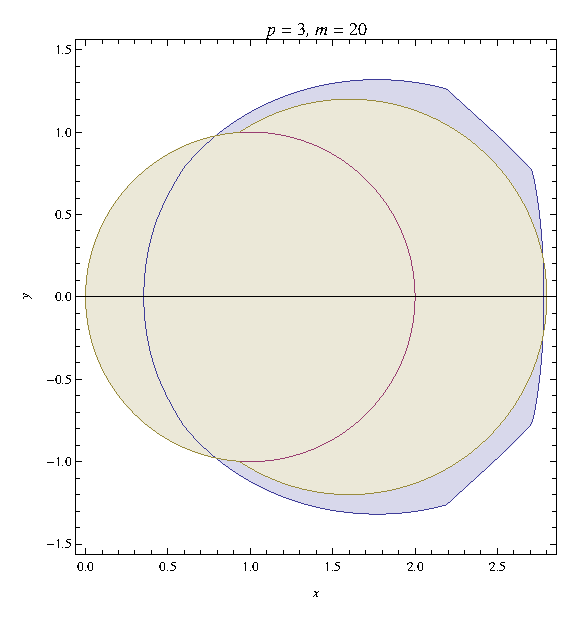
\includegraphics[width=0.3\textwidth]{fig_NM_PraConvReg_p3m20.eps}}
\subfigure[]{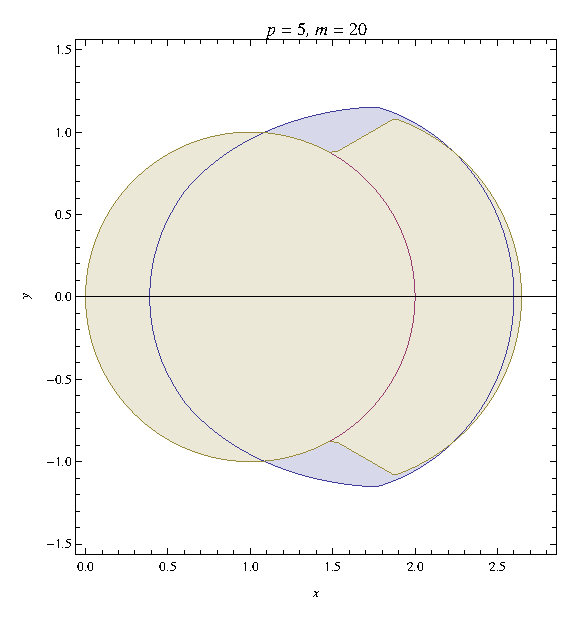
\includegraphics[width=0.3\textwidth]{fig_NM_PraConvReg_p5m20.eps}}
\subfigure[]{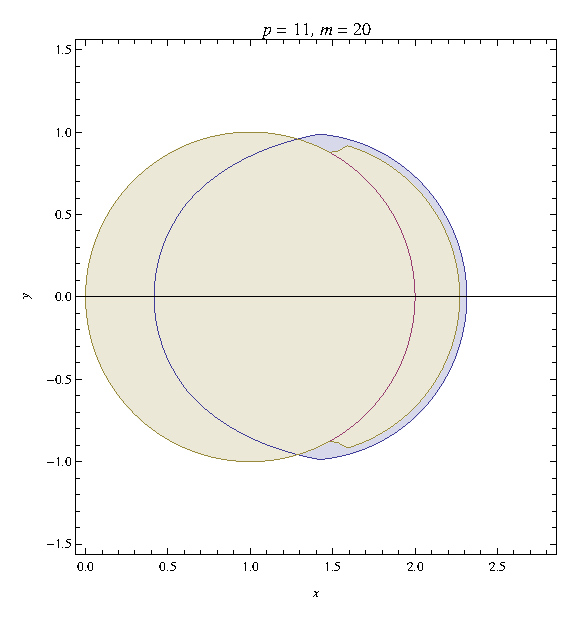
\includegraphics[width=0.3\textwidth]{fig_NM_PraConvReg_p11m20.eps}}\\
\subfigure[]{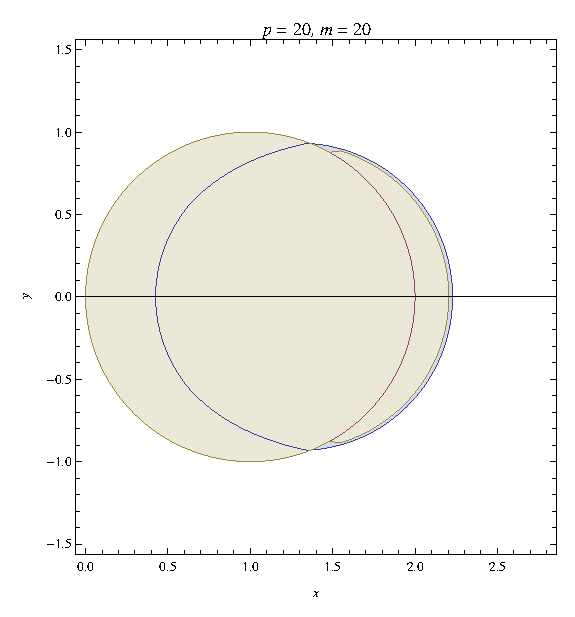
\includegraphics[width=0.3\textwidth]{fig_NM_PraConvReg_p20m20.eps}}
\subfigure[]{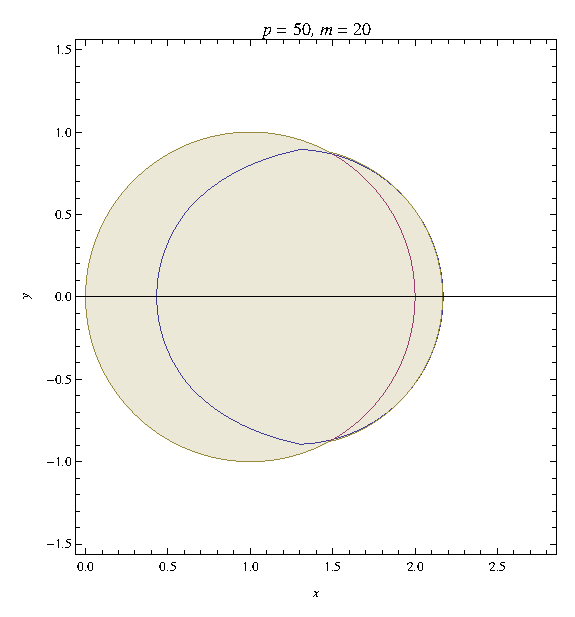
\includegraphics[width=0.3\textwidth]{fig_NM_PraConvReg_p50m20.eps}}
\subfigure[]{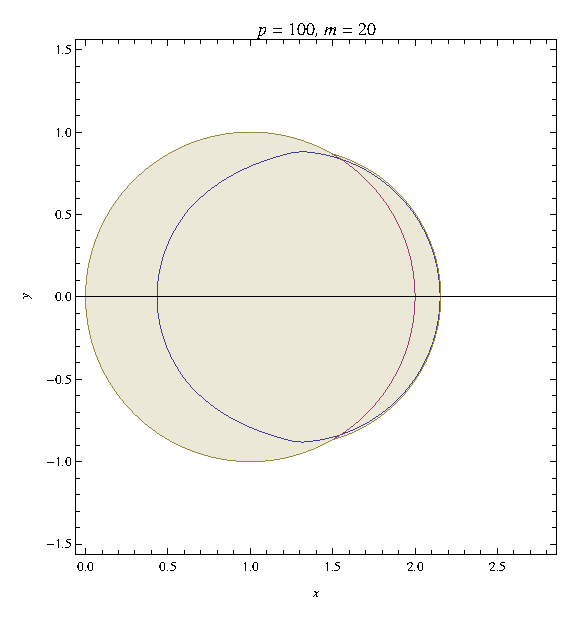
\includegraphics[width=0.3\textwidth]{fig_NM_PraConvReg_p100m20.eps}}\\
\caption{For fixed $m=20$ and $p=2,5,11,20,50,100$, the actual
convergence regions $\MCR_1$ defined in (\ref{set:R_NM}) (the union
of the red and blue parts) and the approximate convergence regions
$\MCR_1^{\text{N}}$ defined in (\ref{set:R_N_pra}) (the yellow
parts).}\label{fig:NM_PraConvReg}
\end{figure}






  %%---------------------------------------------------------------------------------------------------%%
%%------ �����£�����4P1-P1Ԫ���Navier-Stokes���̵��ƶ����񷽷� ------------------------------------%%
%%---------------------------------------------------------------------------------------------------%%


\chapter{����4P1-P1Ԫ���Navier-Stokes���̵��ƶ����񷽷�}
\label{chapter:4P1-P1_moving}

    ������һ��, ����֪�����Ԫ����ⲻ��ѹNavier-Stokes���̵�һ����Ҫ
    ������Ϊ�˱�֤��Ĵ���Ψһ�ԣ���Ҫʹ�ٶȺ�ѹ�����������ڵĿռ�����
    LBB����������һ�ְ취��ʹ���ٶȿռ����ѹ���ռ���˵�����ɶ��㹻�࣬
    ����miniԪ��Taylor-HoodԪ�ȵȡ�����һ�з����Ƕ�ѹ���ռ�ʩ��һЩԼ����
    ����˵�ȶ�����$P_1-P_1$Ԫ��$P_1-P_0$Ԫ��Ϊ�˼��ټ���������߼���Ч�ʣ�ͨ����
    ��������Ӧ���񷽷���������\cite{danaila2014newton},\cite{ebeida2009unsteady}
    \cite{berrone2009space}�У�������h-����Ӧ��P2P1Ԫ����ʵ�ʵĹ��̼�
    ���У�����ͨ��������ʹ������Ԫ�����Ǹߴ�Ԫ��
    \cite{zheng2010posteriori}�������Ӧ������ȶ���P1P1Ԫ��P1P0Ԫ��
    ��ϵIJ���. \cite{di2005moving}���ƶ����񷽷�Ӧ�õ�����ѹNavier-Stokes
    ���̵���⡣�����ƶ����񲿷ֵIJ����ǻ�������\cite{di2005moving}��
    �Ĺ�����Ȼ����������LBB����������Ԫ��Ӧ�õ�����Ӧ���񷽷�����һ���ļ������ѡ�
    �ۺ����Ͽ��ǣ�����ѡȡ�ȶ���$P_1isoP_2P_1$Ԫ������Ȼ����LBB��������ϸ��
    \cite{bercovier1979error}. ��P1ISOP2P1Ԫ���ٶȵ�Ԫ���ڵ����������ѹ
    ��Ԫ���������һ�εõ�����Figure (\ref{fig::p-v})ע�⵽���ٶȵ�Ԫ
    $\vec{u}$ ��ѹ����Ԫ$p$ �Ͼ�������Ԫ�����ǣ��ٶȵ�Ԫ�����ϵ�6����������
    ��ͬһ���ٶȵ�Ԫ�ϡ������ƴװɢ�ȿ���󣬼�ƴװѹ����Ԫ���ٶ�
    ��Ԫ��������̲�����Ȼ��

    �ڱ��ĵĹ����У�����ѡȡ$4P1-P1$Ԫ������$P_1isoP_2P_1$ӵ����ͬ��
    ����ṹ����ȻҲ����inf-sup����������Ҫָ������$P_1isoP_2P_1$Ԫ��
    �ٶȵ�Ԫ�ϵĻ��������ֲ���λ����ͬ���ٶȵ�Ԫ�ڡ��������ƴװɢ��
    ������ṩ�˱�����ֻҪ���ǽ����ĸ��ٶȵ�Ԫ�ʹ��ѹ����Ԫ֮���������
    �����Ľ�����������������������ݽṹ����������������������һ���ᵽ
    �ļ����Ŵ����ṹ�����Խ������������Ķ�Ӧ��ϵ��

    �������������Ŵ����Ľṹ�����ǿ��Ժ����׵Ľ����ĸ�С���ٶȵ�Ԫ��
    ѹ���굥Ԫ���������ͬʱ��\cite{li2005multi}��h-����Ӧ����Ҳ�ǻ�
    ���������ṹ����Ȼ�ģ����ǿ��Խ�h-����Ӧ����Ӧ�õ�4P1-P1Ԫ�ϡ���
    ��Ӧ������Լ��ټ�������ͬʱ�����о�����ֲ�С�߶��ϵ����󣬱���
    �С�ͬʱ���ƶ��������񷽷�Ҳ����Ӧ����4P1-P1Ԫ�ϣ������ƶ�����ֻ
    �ƶ�ѹ�����񣬵�ѹ�������ƶ��꣬�ٶ�������ѹ���������һ�μ��ɵ�
    ����������Ҫע����ǣ���ⲻ��ѹ��Navier-Stokes���̣��ڽ��������
    ���ֵ���ƶ��������Ĺ��̣�Ҫ����ɢ��Ϊ0�����������������
    \cite{di2005moving}�����

    �ڵ�һ���У����ǽ���Navier-Stokes���̵�֪ʶ��
    �ڵڶ���������չʾ4P1-P1�����ݽṹ���Լ���Ԫ�������Ľ������̣�������
    ������4P1-P1Ԫ����Navier-Stokes���̡��ƶ�����IJ��Խ��ڵ��Ľ��и�����
    ������Ǹ�����ֵ���ӡ�

\section{���ݽṹ}
   4P1-P1�ǻ������ײ�ͬ���������������Ԫ�ռ䡣�ٶ����������ѹ������
   ȫ�ּ���һ�εõ�����������ݽṹ�ǻ���\cite{li2005multi}�еļ�����
   �����ṹ����Figure(\ref{fig::hgrometrytree})��ʾ��һ����ѹ����Ԫ��
   Ӧ���ĸ��ٶȵ�Ԫ��ͨ������һ�����е��ٶȵ�Ԫ�����ü����Ŵ����ṹ��
   �Ϳ��Խ����ٶȵ�Ԫ��ѹ����Ԫ��$1-1$��Ӧ��

   ��AFEPack�У��ٶ������ѹ������ֱ�洢�����ŷ���������irregularMeshV
   ��irregularMeshP�ϣ������ŷ����������ǽ�����ͬһ�����ϡ������������ϣ�
   ���Խ���ȫ�ּ��ܣ��ֲ������Լ��軯�IJ������ܽ������ֲ��������������IJ����ṹ��
   ���е�����ڵ�Ӹ��ڵ㵽Ҷ�ӽڵ㣬���洢�ڷ����������С�����irregularMeshV
   ����irregularMeshP����ȫ��һ�μ��ܵõ��ģ����ݷ�������������ṹ�����ǿ���
   ͨ������irregularMeshV��ȫ�����Ԫ(��Ҷ�ӽڵ�)��ͨ�����Ԫ���ҵ�����
   ���׵�Ԫ(��Ҷ�ӽڵ�ĸ��׽ڵ�)���������ǽ����˴��ٶ�����Ԫ��ѹ������Ԫ
   ֮��ĵ������������Ǹ��ݻ��Ԫ�ĸ��׽ڵ�Ҳ�Ǿ������ṹ�ģ���ˣ����ǿ���
   ���ݸ��ӽڵ㵥Ԫ(ѹ����Ԫ)���ҵ�����Ӧ���ĸ����ӵ�Ԫ(���ĸ��ٶȵ�Ԫ)������
   ����Ҳ�����˴�ѹ����Ԫ���ٶȵ�Ԫ�ĵ���������������ٶȺ�ѹ����ĵ�Ԫ�Ѿ�������
   $1-1$������ע�⵽��ֻҪ�������µ�����Ԫ�����ǽ�������������Ҫ���¸ġ�Ӧ�õ�
   �ƶ������ϣ�����ֻ��Ҫһ�ι��������Ϳ��ԣ�������������ƶ�����������������ı䡣
   ���������Ĺ��̲μ��㷨(\ref{alg::index})��


   \begin{algorithm}
     \caption{�����ٶȵ�Ԫ��ѹ����Ԫ�������}
     \begin{algorithmic}[n]
%     \begin{list}[1]
       \State \text{achieveiterator} $\gets$ \text{irregualerMeshV.beginActiveElement()}
       \State \text{enditerator} $\gets$ \text{irregualerMeshV.endActiveElement()}

       \While {\text{achieveiterator} $\neq$ \text{enditerator}}
           \State \text{int index-v-element} $\gets$
                   \text{achieveiterator}$-\rangle$ \text{index}
           \State \text{HElement} $\langle$ \text{DIM,
                   DIM}$\rangle \ast$ \text{parent} $\gets$
                   \text{activeiterator}$-\rangle$ \text{parent}
           \State \text{int index-p-element} $\gets$
                   \text {parent}$-\rangle$ \text{index}
           \State \text{int n-child} $\gets$
                   \text{parent}$-\rangle$ \text{n-child}
           \State
                  \text{index-p2v[index-p-element].resize}(\text{n-child})
           \While {$i \geq 0$ \textbf{and} $i < \text{n-child}$}
                  \State \text{HElement}$\langle$\text{DIM,DIM}$\rangle$ $\ast$\text{chi}
                         $\gets$ \text{parent}$-\rangle$\text{child[i]}
                  \State \text{int index-v-element} $\gets$
                         \text{child}$-\rangle$\text{index}
                  \State \text{index-p2v[index-p-element][i]} $\gets$
                         \text{index-v-element}
                  \State \text{index-v2p[index-v-element]} $\gets$ \text{index-p-element}
           \EndWhile
       \EndWhile
     \end{algorithmic}
%     \end{list}
     \label{alg::index}
   \end{algorithm}


\section{���Ԫ����}
    \subsection{���巽��}
        ��Stokes����
        \begin{equation}
            \begin{aligned}
                -\bigtriangleup \vec{u} + \nabla p = f \quad \text{��}\Omega \text{��}, \\
                \nabla \cdot \vec{u} = 0 \quad \text{��}\Omega \text{��},\\
                \vec{u} = 0 \qquad \text{��}\partial \Omega \text{��},
            \end{aligned}
            \label{eq::stokes}
        \end{equation}
        �Ļ����ϼ�һ��������ټ���ʱ������ǿ��Եõ�һ��ʱ�䷢չ��Navier-Stokes����
        \begin{equation}
            \begin{aligned}
                \frac{\partial \vec{u}}{\partial t}-\nu \nabla^2\vec{u} + \vec{u}\cdot \nabla \vec{u} + \nabla p &=& \vec{f}, \\
                \nabla \cdot \vec{u} = 0.
            \end{aligned}
            \label{eq::NS_system}
        \end{equation}
        ����$\nu > 0$ ��һ����������������ѧճ��ϵ������Stokes ���������ƣ�$\vec{u}$��ʾ�����ٶȣ�
        $p$��ʾѹ����������$\vec{u} \cdot \nabla \vec{u} := (\vec{u} \cdot \nabla) \vec{u}$���Ƿ�
        �������Ҳʹ��Navier-Stokes���̵ĽⲻΨһ����Ҳ�����ǵ���ֵ���������һ������ս��
        ϵͳ(\ref{eq::NS_system})�ļ���������$\Omega$�������Ƕ�ά�Ļ���ά�ġ��ڱ߽�$\partial \Omega =
        \partial \Omega_D \cup \Omega_N$�ϵı߽��������£�
        \begin{equation}
            \begin{array}{ll}
                \vec{u} = \vec{w},& \mbox{ on } \partial \Omega_D,\\
                \nu \displaystyle \frac{\partial \vec{u}}{\partial n} - p =
                \vec{0}, & \mbox{ on } \partial \Omega_N.  \\
             \end{array}
            \label{eq::bc}
        \end{equation}
        ���б߽�$\partial \Omega = \partial \Omega_D \bigcup \partial \Omega_N$,
        $\vec{n}$��ʾ�߽���ⷨ��
        Dirichlet�߽���ݱ߽��ϵ��ٶȺ��ⷨ��ij˻�������ϸ��Ϊ��
        \begin{equation}
            \begin{aligned}
                \partial \Omega_{+} = {x \mbox{��} \partial \Omega \mbox{��}|\vec{\omega} \cdot \vec{n} > 0}, \quad \mbox{�����߽�}��\\
                \partial \Omega_{0} = {x \mbox{��} \partial \Omega \mbox{��}|\vec{\omega} \cdot \vec{n} = 0}, \quad \mbox{�����߽�}��\\
                \partial \Omega_{-} = {x \mbox{��} \partial \Omega \mbox{��}|\vec{\omega} \cdot \vec{n} < 0}, \quad \mbox{�����߽�}��\\
            \end{aligned}
        \end{equation}
        ����߽�ȫ����Direchlet�߽���������$\partial \Omega = \partial \Omega_D$����ôNavier-Stokes����
        (\ref{eq::NS_system})��(\ref{eq::bc})��ѹ�����ȥһ����������Ψһ�ġ�
        ���Ƕ�(\ref{eq::NS_system})�еIJ���ѹԼ��Ӧ��ɢ�ȶ�����
        \begin{equation}
            0 = \int_{\Omega} \nabla \cdot \vec{u} = \int_{\partial \Omega} \vec{u} \cdot \vec{n} = \int_{\Omega} \vec{\omega} \cdot \vec{n}.
        \end{equation}
        ���߽�ֵҪ��������������
        \begin{equation}
            \int_{\partial \Omega_{+}} \vec{\omega} \cdot \vec{n} + \int_{\partial \Omega_{-}} \vec{\omega} \cdot \vec{n} = 0.
        \end{equation}
        �򵥵Ľ�������˵����$\Omega$������������Ҫ�������������ȡ���Ҳ��ѹ����Ψһ��ԭ���ڴ�������/����������ʱ��Ҫע�Ᵽ
        ֤�������������������Navier-Stokes����Ľ��п��ܲ����ڡ�һ������£������ڳ����߽�������Ȼ��������������������Ȼ���㣬���
        ��ʱ������(\ref{eq::NS_system})��(\ref{eq::bc})��ѹ������Ψһ�ġ�

        (\ref{eq::NS_system})��Navier-Stokes��ԭʼ������ʽ,��������һ�������ʽ����������ʽ���������$\Omega$�ǵ���ͨ�ģ���ô����ѹ������
        \begin{equation}
            \frac{\partial u_x}{\partial x} = -\frac{\partial u_y}{\partial y}
        \end{equation}
        ��ζ�Ŵ���һ��������$\psi(x, y)$ ʹ��
        \begin{equation}
            u_x = \frac{\partial \psi}{\partial y}, \quad u_y = -\frac{\partial \psi}{\partial x}.
        \end{equation}
        $\psi(x, y)$��ȥһ�������ⱻ$\vec{u}$Ψһȷ����
        ��(\ref{eq::NS_system})�еĶ�������ȡcurl�����ǿ��Եõ���������ʽ��
        \begin{equation}
            -\nu \nabla^4 \psi + \frac{\partial \psi}{\partial y}\frac{\partial}{\partial x}(\nabla^2\psi) - \frac{\partial \psi}{\partial x}\frac{\partial }{\partial y}(\nabla^2 \psi) = -curl \vec{f}
            \label{eq::stream_line}
        \end{equation}
        ��������������ʽ(\ref{eq::stream_line})����ά�ռ�û��һ����ʽ��������������ʽֻ�ڶ�ά�����ǻ����о�(\ref{eq::NS_system})�е�ԭʼ
        ������ʽ��
    \subsection{����ʽ}
        ���Ƕ����ͼ���ռ����£�
        \begin{eqnarray}
            \mathbf{H}_E^1 & := & \left\{ \vec{u} \in \mathcal{H}^1(\Omega)^d \big|
            \vec{u} = \vec{w} \mbox{ on } \partial \Omega_D \right\},\\
            \mathbf{H}_{E_0}^1 & := & \left\{ \vec{v} \in \mathcal{H}^1(\Omega)^d \big|
            \vec{u} = \vec{0} \mbox{ on } \partial \Omega_D \right\}.
        \end{eqnarray}
        ��ô�����ʽΪ��Ѱ��$(\vec{u}, p) \in (\mathbf{H}_E^1,
        L_2(\Omega))$ ʹ��
        \begin{eqnarray}
             \int_{\Omega}\frac{\partial \vec{u}}{\partial t} \cdot \vec{v} +
            \nu \int_\Omega \nabla \vec{u} : \nabla \vec{v} + \int_\Omega \left(
            \vec{u} \cdot \nabla \vec{u} \right) \cdot \vec{v} - \int p
            \left( \nabla \cdot \vec{v} \right) & = & \int_\Omega \vec{f} \cdot
            \vec{v}, \label{eq::generalweak_momentum}\\
             & & \forall \vec{v} \in \mathbf{H}_{E_0}^1,\notag \\
             \int_\Omega q \left( \nabla \cdot \vec{u} \right) & = & 0,
             \label{eq::generalweak_mass} \\
            & & \forall q \in L_2(\Omega). \notag
       \end{eqnarray}

       ����$\nabla \vec{u} : \nabla \vec{v}$ ��ʾ�����ij˻����ڶ�ά��Ϊ
       $\nabla u_x \cdot \nabla v_x + \nabla u_y \cdot \nabla v_y$.
       �����ڹ�����Ԫ���Ƶ�ʱ��Ҫȷ���ɽ�������
       \begin{equation}
            \int_{\Omega}p \nabla \cdot \vec{v} = 0 \quad \text{�������}\vec{v} \in \mathbf{H}_{E_0}^1 \Rightarrow \left\{ \begin{array}{ll}
                p = \mbox{constant} & \text{���} \partial \Omega = \partial \Omega_D \\
                p = 0 & \text{�������}
            \end{array}
            \right.
            \label{eq::solve_condition}
       \end{equation}
        (\ref{eq::solve_condition})������inf-sup �����Ƴ���
        \begin{equation}
            \inf_{ q \neq \mbox{constant}} \sup_{\vec{v} \neq \vec{0}} \frac{|(q, \nabla \cdot \vec{v})|}{||vec{v}||_{H(\Omega)^1} ||q||_{L(\Omega)^0}} \geq \gamma > 0.
        \end{equation}

       ����$\tau_h$��$\Omega$ �϶�ѹ������������ʷ֣�����߶� $h = max_{T
         \in \tau_h} diam(T)$, $T$ Ϊ�����ʷ� $\tau_h$ �ĵ�Ԫ����Ӧ�ģ�
       $\tau_{\frac{h}{2}}$ �Ƕ��ٶ�����������ʷ֡�����
       $\tau_{\frac{h}{2}}$ �� $\tau_{h}$ �ϵ�����Ԫ�ռ� $X_E^h$ �� $P_h$
       ����
       \begin{equation}
         X_E^h \subset \mathcal{H}_E, \quad P_h \subset L_2(\Omega)
         \notag
       \end{equation}

       ��ô(\ref{eq::generalweak_momentum}) �� (\ref{eq::generalweak_mass})
       ����д��������ʽ: Ѱ�� $(\vec{u}_h, p_h) \in X_E^h \times P_h$ ʹ��
       \begin{equation}
         \begin{aligned}
           &\int_{\Omega}\frac{\partial \vec{u}_h}{\partial t} \cdot \vec{v}_h
           + \nu \int_\Omega \nabla \vec{u}_h : \nabla \vec{v}_h  \\
           + & \int_\Omega \left( \vec{u}_h \cdot \nabla \vec{u}_h \right)
           \cdot \vec{v}_h - \int_\Omega p_h \left( \nabla \cdot \vec{v}_h
           \right) & = &\int_\Omega \vec{f} \cdot \vec{v}_h, &\quad
           \forall \vec{v}_h \in \mathbf{X}_0^h;  \\
           & \int_\Omega q_h \left( \nabla \cdot \vec{u}_h \right) & = &0,&
           \quad \forall q_h \in P^h.
           \label{eq::discreted_weak}
         \end{aligned}
       \end{equation}

   Ϊ�˼�㣬����ʱ����ɢ������ʾEuler��ʽ��
   $\forall (\vec{v}_h, q_h) \in \mathbf{X}_0^h \times P^h$
   \begin{equation}
     \begin{aligned}
       \int_{\Omega} \frac{\vec{u}_h^{(n + 1)} -
         \vec{u}_h^{(n)}}{\delta t} \cdot \vec{v} + \nu \int_{\Omega} \nabla
       \vec{u}_h^{(n + 1)} : \nabla \vec{v}_h - \int_{\Omega} p_h^{(n
         + 1)} \left( \nabla \cdot \vec{v}_h \right)
       & = \int_{\Omega}\left(\vec{f} + \vec{u}_h^{(n)} \cdot \nabla \vec{u}_h^{(n)}
       \right) \cdot \vec{v} &\\
       \int_{\Omega} q_h \nabla \cdot \vec{u}_h^{(n + 1)} & = 0.&
     \end{aligned}
     \label{eq::time_discreted_weak}
   \end{equation}
   �� $\{\phi_j \}_{j = 1}^n$ �� $\{\psi_k\}_{k = 1}^m$ �ֱ�Ϊ�ٶȺ�ѹ
   ��������Ԫ������������ֵ��$\vec{u}_h^{(n + 1)} = (u_{xh}^{(n + 1)},
   u_{yh}^{(n + 1)}), p_h$ ����д��������ʽ��
   \begin{equation}
     u_{xh}^{(n + 1)} = \sum_{j = 1}^n u_j \phi_j, \quad u_{yh}^{(n +
       1)} = \sum_{j = 1}^n v_j \phi_j, \quad p_h^{(n + 1)} = \sum_{k
       = 1}^m p_k \psi_k \notag
   \end{equation}
   ��$u_{xh}^{(n + 1)}, u_{yh}^{(n + 1)}, p_h^{(n + 1)}$������ɢ����ʽ
   (\ref{eq::time_discreted_weak}) ������
   �õ����Է�����
   \begin{equation}
     \left[
       \begin{array}{lll}
         \frac{1}{dt} M + \nu A & 0 & B_x^T \\
         0 & \frac{1}{dt} M +\nu A  & B_y^T \\
         B_x & B_y & 0
       \end{array}
     \right]
     \left[
       \begin{array}{c}
         u_x \\
         u_y \\
         p
       \end{array}
     \right] =
     \left[
       \begin{array}{c}
         f_x \\
         f_y \\
         g
       \end{array}
     \right],
     \label{eq::linear_system}
   \end{equation}
   ����M �� $n \times n$ ����������A��������˹������������ʽ��
   \begin{eqnarray}
     A & = & [a_{ij}], \quad a_{ij} = \int_\Omega \nabla \phi_i \cdot \nabla
     \phi_j  \notag \\
     M & = & [m_{ij}], \quad m_{ij} = \int_{\Omega}\phi_i \phi_j \notag \\
     B_x^T & = & [bx^T_{ik}], \quad bx^T_{ik} = \int_{\Omega} \psi_k
     \frac{\partial{\phi_i}}{\partial x}  \notag \\
     B_y^T & = & [by^T_{ik}], \quad by^T_{ik} = \int_{\Omega} \psi_k
     \frac{\partial {\phi_i}}{\partial y}  \notag \\
     f_x & = & [f_i], \quad f_i = \int_\Omega (\frac{u_{xh}^{(n)}}{dt} - (u_{xh}^{(n)}
     \frac{\partial u_{xh}^{(n)}}{\partial x} + u_{yh}^{(n)} \frac{\partial
       u_{xh}^{(n)}}{\partial y}) \phi_i \notag \\
     f_y & = & [f_i], \quad f_i = \int_\Omega (\frac{u_{yh}^{(n)}}{dt} - (u_{xh}^{(n)}
     \frac{\partial u_{yh}^{(n)}}{\partial x} + u_{yh}^{(n)} \frac{\partial
       u_{yh}^{(n)}}{\partial y}) \phi_i \notag \\
     g & = &  [g_k],\quad  g_i = 0. \notag
   \end{eqnarray}

   �������������ؽ���һ��ɢ�ȿ����$B_x B_y, B_x^T, B_y^T$��ƴװ�� ��
   $B_x^T$Ϊ��, ��$\triangle_{v_i}$ Ϊһ���ٶȵ�Ԫ�����ǿ���ͨ����һ�ڽ�����
   ��Ԫ�������ҵ���Ӧ��ѹ����Ԫ $\triangle_{p_k}$(�� Figure
   (\ref{fig::matrix_assemble})). $\phi_{i_1}, \phi_{i_2}, \phi_{i_3}$
   �Ƕ������ٶȵ�Ԫ $\triangle_{v_i}$ �ϵ�����Ԫ���������±� $i_1,
   i_2, i_3$ ��ʾ�ö����ϵ����ɶ����ٶ�ȫ�����ɶȵ�ȫ�ֱ�š�ͬʱ
   $\psi_{k_1}, \psi_{k_2}, \psi_{k_3}$ �Ƕ�����ѹ����Ԫ
   $\triangle_{p_k}$ �ϵ�����Ԫ��������$k_1, k_2, k_3$ ������Ԫ
   $\triangle_{p_k}$ �ϵ����ɶ���ѹ��ȫ�����ɶ��е�ȫ�ֱ�š�
   ��� ��Ԫ $\triangle_{p_k}$ �� $\triangle_{v_i}$ �� $B_x^T$ �Ĺ���
   Ϊ
   \begin{equation}
     \left[
     \begin{array}{lll}
       \int_{\triangle_{v_i}}\psi_{k_1} \frac{\partial
         \phi_{i_1}}{\partial x} & \int_{\triangle_{v_i}} \psi_{k_2}
       \frac{\partial \phi_{i_1}}{\partial x} & \int_{\triangle_{v_i}}
       \psi_{k_3} \frac{\partial \phi_{i_1}}{\partial x} \\
       \int_{\triangle_{v_i}} \psi_{k_1} \frac{\partial
         \phi_{i_2}}{\partial x} & \int_{\triangle_{v_i}} \psi_{k_2}
       \frac{\partial \phi_{i_2}}{\partial x} & \int_{\triangle_{v_i}}
       \psi_{k_3} \frac{\partial \phi_{i_2}}{\partial x} \\
       \int_{\triangle_{v_i}} \psi_{k_1} \frac{\partial
         \phi_{i_3}}{\partial x} & \int_{\triangle_{v_i}} \psi_{k_2}
       \frac{\partial \phi_{i_3}}{\partial x} & \int_{\triangle_{v_i}}
       \psi_{k_3} \frac{\partial \phi_{i_3}}{\partial x}
     \end{array}
   \right]
   \label{eq::element_matrix}
   \end{equation}

   �����׾��� (\ref{eq::element_matrix}) �ӵ� $B_x^T$ �е���Ӧλ��
   $(i_1,k_1)$, $(i_1, k_2)$, $(i_1, k_3)$, $(i_2, k_1)$, $(i_2, k_2)$,
   $(i_2,k_3)$, $(i_3, k_1)$, $(i_3, k_2)$, $(i_3, k_3)$ to  $B_x^T$.
   �ϡ�ͨ���������е��ٶȵ�Ԫ���ظ�����IJ�����$B_x^T$ ƴװ��ɡ�
   $B_y^T$ Ҳ����ͬ��ƴװ��

   $B_x$ �� $B_y$ ��ƴװ�DZ������е�ѹ����Ԫ��ͨ����Ԫ�������ҵ���Ӧ��
   �ĸ��ٶȵ�Ԫ��Ȼ��ֱ���ѹ����Ԫ���ĸ��ٶȵ�Ԫ����ƴװ���������ƣ�
   �㲻��׸����
   \begin{figure}
     \centering
     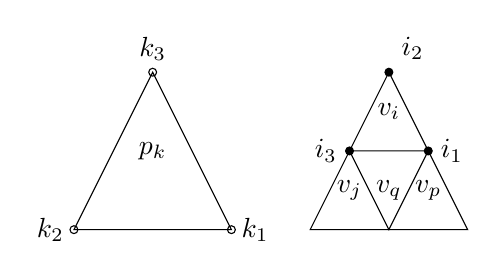
\begin{tikzpicture}
       % ������
       \draw (2, 1) -- (4, 1) -- (3, 3) -- cycle;
       % ��������
       \draw (2, 1) circle(0.05cm);
       \draw (4, 1) circle(0.05cm);
       \draw (3, 3) circle(0.05cm);
       \draw (3, 2) node{$p_k$};
       % ����������.
       \draw (1.7, 1) node {$k_2$};
       \draw (4.3, 1) node {$k_1$};
       \draw (3, 3.3) node {$k_3$};
       % �ĸ�������
       \draw (5, 1) -- (6, 3) -- (7, 1) -- cycle;
       \draw (5.5, 2) -- (6.5, 2) -- (6, 1) -- cycle;
       % ��������
       \draw [fill = black](6.5, 2) circle(0.05cm);
       \draw [fill = black](5.5, 2) circle(0.05cm);
       \draw [fill = black](6, 3) circle(0.05cm);
       % ����������.
       \draw (6.8, 2) node {$i_1$};
       \draw (6.3, 3.3) node {$i_2$};
       \draw (5.2, 2) node {$i_3$};
       % ��Ԫ���.
       \draw (6, 2.5) node {$v_i$};
       \draw (5.5, 1.5) node {$v_j$};
       \draw (6.5, 1.5) node {$v_p$};
       \draw (6, 1.5) node {$v_q$};
     \end{tikzpicture}
     \caption{��: $p$ ��Ԫ; ��: ��ѹ����Ԫ��Ӧ��4���ٶ�$v$��Ԫ }
     \label{fig::matrix_assemble}
   \end{figure}
   \section{Ԥ��������}
      �����ǵ����Navier-Stokes���̵��㷨�У���������̬��Stokes���̵Ľ���Ϊ��ʼֵ���������һ�����У����ǿ������
      Stokes ���̵�Ԥ��������������д��\eqref{eq::stokes}��$4P1-P1$���Ƶ���ɢ����ʽ��Ѱ�� $(\vec{u}_h, p_h) \in X_E^h \times P_h$
      ʹ��
       \begin{equation}
         \begin{aligned}
           \nu \int_\Omega \nabla \vec{u}_h : \nabla \vec{v}_h
           - \int_\Omega p_h \left( \nabla \cdot \vec{v}_h
           \right) & = \int_\Omega \vec{f} \cdot \vec{v}_h, \quad
           \forall \vec{v}_h \in \mathbf{X}_0^h,&  \\
           \int_\Omega q_h \left( \nabla \cdot \vec{u}_h \right) & = 0,
           \quad \forall q_h \in P^h.&
           \label{eq::discreted_weak_stokes}
         \end{aligned}
       \end{equation}
      ͬ���ģ��� $\{\phi_j \}_{j = 1}^n$ �� $\{\psi_k\}_{k = 1}^m$ �ֱ�Ϊ $X_E^h$ ��$\times P_h$�Ļ�����������ֵ��
      $\vec{u}_h^{(n + 1)} = (u_{xh}^{(n + 1)}, u_{yh}^{(n + 1)}), p_h$ ����д��������ʽ��
      \begin{equation}
         u_{xh}^{(n + 1)} = \sum_{j = 1}^n u_j \phi_j, \quad u_{yh}^{(n +
         1)} = \sum_{j = 1}^n v_j \phi_j, \quad p_h^{(n + 1)} = \sum_{k
         = 1}^m p_k \psi_k \notag
      \end{equation}
      ��$u_{xh}^{(n + 1)}, u_{yh}^{(n + 1)}, p_h^{(n + 1)}$������ɢ����ʽ
      (\ref{eq::time_discreted_weak}) ������
      �õ����Է�����
       \begin{equation}
         \left[
           \begin{array}{lll}
             \nu A & 0 & B_x^T \\
             0 & \nu A  & B_y^T \\
             B_x & B_y & 0
           \end{array}
         \right]
         \left[
           \begin{array}{c}
              u_x \\
              u_y \\
              p
           \end{array}
         \right] =
         \left[
           \begin{array}{c}
             \hat{f}_x \\
             \hat{f}_y \\
             \hat{g}
           \end{array}
         \right],
         \label{eq::linear_system_stokes}
       \end{equation}
     Ϊ��������������(\ref{eq::linear_system_stokes})�е��Ҷ���ֱ�ȡΪ
     $\hat{f}_x = 0, \hat{f}_y = 0, \hat{g} = 0$������ѡ��MINRES(��С���в��)�����\eqref{eq::linear_system_stokes}��ͨ������£�
     ����ҪΪMINRESѡ��һ����Ч��Ԥ�����ӡ���\cite{elman2005finite}�У����ѹ���ռ����������:
     \begin{equation}
        Q  =  [Q_{ij}], \quad q_{ij} = \int_\Omega \nabla \psi_i \cdot \nabla \psi_j  \notag
     \end{equation}
     ������Ϊschur��$S = B_x A^{-1} B_x^T + B_y A^{-1} B_y^T$�Ľ��ƾ�����ʵ�ʵļ����У�ѹ����������ĶԽ���$\hat{Q} = diag(Q)$������
     �бȽϺõ�Ч������ˣ�����ѡȡ�Խǿ����$K$
       \begin{equation}
         K = \left[
               \begin{array}{lll}
                 \nu A & 0 & 0 \\
                 0 & \nu A  & 0 \\
                 0 & 0 & \hat{Q}
               \end{array}
             \right]
       \end{equation}
       ��Ϊ(\eqref{eq::linear_system_stokes})��ϵ������$M$�Ľ��ơ�
       \begin{equation}
         M = \left[
               \begin{array}{lll}
                 \nu A & 0 & B_x^T \\
                 0 & \nu A  & B_y^T \\
                 B_x & B_y & 0
               \end{array}
             \right],
       \end{equation}
   ��Ԥ���������У�������Ҫ�Ծ���$K$���棬����� $V_{dst} = K^{-1} V_{src}$�IJ�����
   ����$V_{dst}, V_{src}$ �ֱ�Ϊ
   \begin{equation}
      V_{dst} = (V_{dst}^x, V_{dst}^y, V_{dst}^p)^T,\quad V_{src} = (V_{src}^x, V_{src}^y, V_{src}^p)^T.
   \end{equation}
   ���Dz���ֱ����� $V_{dst} = K^{-1} V_{src}$�����ǰ�$K$�ֳ������Խǿ� $(0, 0)$��$(1, 1)$ �� $(2, 2)$�飬
   Ȼ��ÿ������е�����⡣������Ӧ����possion����Ĵ���������������������
   \begin{eqnarray}
      \nu A V_{des}^x = V_{src}^x, \notag \\
      \nu A V_{des}^y = V_{src}^y. \notag
   \end{eqnarray}
   ���� $(2, 2)$ �飬
   \begin{equation}
      V_{dst}^p = \frac{V_{src}^p}{diag(\hat{Q})}
   \end{equation}
   ��ô���Ǿ͵õ���$V_{dst}$��

\section{�ƶ��������}

   ������Ҫ���뷨�������������ٶ������ѹ�������ٶ����������ѹ��
   �������һ�εõ���������Ƕ�ѹ����������ƶ���Ȼ����ƶ����ѹ����
   ��ȫ�ּ���һ�Σ�����ʵ�ֶ��ٶ������ͬ���ƶ���

   �� $t = t_{n + 1}$ ʱ�̣� ����һ�µķ������Եõ�����Ԫ��
   $(\vec{u}_h^{(n + 1)}, p_h^{(n + 1)})$. �����������������µ���ֵ
   ��;ɵ�����$\mathcal {T}_h^{(n)}$ ������µ�����$\mathcal {T}_h^{(n +
   1)}$. ���Dz�ȡ���� \cite{di2005moving} �еķ�����ע�⵽��������ı�
   �����Dirichlet�߽磬��Ϊ�����IJ���
   \subsection{Step 1 ��ȡMonitor}
     ѡ��һ�����ʵĿ��ƺ����������ƶ�����Ľ���Ƿdz���Ҫ�ġ�Ӧ���ڲ�
     ��ѹNavier-Stokes�����ϵĿ��ƺ�����Ҫ�����¼���.
     �� $m = \frac{1}{G}$ ����$m$��(\ref{eq::logical})�е�һ������������
     ����$G$�м��в�ͬ��ѡ��.һ���ǻ�������
     \begin{equation}
       G_0 = \sqrt{1 + \alpha |\omega|^\beta}
       \label{eq::monitor_vorticity}
     \end{equation}
     ����$\omega = \nabla \times \vec{u}$, $\alpha$��$\beta$����������
     ������

      ����һ��ѡ��$G$�ǻ�����ֵ����ݶ�
      \begin{equation}
        G_1 = \sqrt{1 + \alpha |\nabla \vec{u}|^\beta}
        \label{eq::monitor_gradient}
      \end{equation}

      ��������Ԫ$v_h$�ƽ���ʵ��$v$������ĺ��������ƹ�ʽ������������
      �������
      \begin{equation}
        |v - v_h|_{1, \Omega} \sim \eta(v_h) := \sqrt{\sum\limits_{l:
            \text{�ڲ��߽�}} \int_l \left[ \nabla v_h \cdot \vec{n}_l
            \right]^2 dl}
      \end{equation}
      ����$[\cdot]_l$��ζ�ű�$l$�ϵ���Ծ����$[v]_l = v|_{l^{+}} -
      v|_{l^{+}}$. ����Ȼ����ÿ����Ԫ�ϵȷֲ���ֵ���$\eta(v_h)$, ����
      ����Ϊһ����ʽ
      \begin{equation}
        G_2 = \sqrt{1 + \alpha \eta^2(v_h)}
        \label{eq::monitor_posterror}
      \end{equation}
      \cite{di2005moving}�ж�(\ref{eq::monitor_posterror})�����˸Ľ�
      \begin{equation}
        G_3 = \sqrt{1 + \alpha \left[ \eta(v_h) / \text{max}\eta(v_h)
          \right]^\beta}
        \label{eq::monitor_posterror_modified}
      \end{equation}
      ����$\beta > 2$ʱ�и��õ�Ч����

   \subsection{Step 2 ��ȡ�µ��߼�����}
     �����Բ�η���
     \begin{eqnarray}
       \begin{aligned}
         \nabla_{\vec{x}} \left ( m \nabla_{\vec{x}} \vec{\xi} \right)
         = 0 \\
         \vec{\xi} = \vec{\xi}_b
       \end{aligned}
       \label{eq::logical}
     \end{eqnarray}
     ���� $m$ ����һ���еĴ���������ͨ��������$(\vec{u}_h^{(n + 1)},
     p_h^{(n + 1)})$�����Ƕ����ʼ���߼�����$\mathcal{T}_c (\mathcal
     {A}^{0} \text{Ϊ���Ľڵ�})$��һ����ʼ���߼���������������������
     �����У���һֱ���ֲ��䡣ͨ�����(\ref{eq::logical}) ���ǿ��Եõ�
     �µ��߼�����$\mathcal{T}_c^*$($\mathcal{A}^*$Ϊ���Ľڵ�)��
  \subsection{Step 3 ����������ƶ�����}

     ����������һЩ���塣$\mathcal{T}_h$ Ϊ���������ϵ������ʷ֡���i��
     �㶨��Ϊ$X_i$����$X_i$ Ϊ����ĵ�Ԫ�ļ��ϳ�֮Ϊ$T_i$����Ӧ�ļ���
     �����ϵı��Ϊ $\mathcal{T}_c, \mathcal{A}_i$ �� $T_{i,c}$��
     $\mathcal{A}_i$ ���ڼ��������ϵ����궨��Ϊ $(\mathcal{A}_i^1,
     \mathcal{A}_i^2)^T$���� Step 1 ���������ǵõ����µ��߼�����
     $\mathcal{T}_c^*$ �����Ķ��� $\mathcal{A}_i^*$. �Ӷ����ǵõ��¾�
     �߼�����IJ�:
     \begin{equation}
       \delta \mathcal{A}_i  = \mathcal{A}^{(0)} - \mathcal{A}_i^*
     \end{equation}
     ����һ�������ĵ�Ԫ$E \in \mathcal{T}_h$, $X_{E_k}, 0 \leq k \leq
     2 $, ��Ϊ�����������㡣��$V_{\mathcal{T}_c^*}(\Omega)$ ��
     $V_{\mathcal{T}}(\Omega)$ �ķ�Ƭ����ӳ���ڵ�Ԫ $E$ �ϵ��ݶ��dz�����
     ������������ķ����飺
     \begin{eqnarray}
       \begin{aligned}
        & \left (
           \begin{array}{cc}
             \mathcal{A}_{E_1}^{*, 1} - \mathcal{A}_{E_0}^{*, 1} &
             \mathcal{A}_{E_2}^{*, 1} - \mathcal{A}_{E_0}^{*, 1} \\
             \mathcal{A}_{E_1}^{*, 2} - \mathcal{A}_{E_0}^{*, 2} &
             \mathcal{A}_{E_2}^{*, 2} - \mathcal{A}_{E_0}^{*, 2}
           \end{array}
         \right )
         \left (
           \begin{array}{cc}
             \frac{\partial x^1}{\partial \xi^1} & \frac{\partial
               x^1}{\partial \xi^2} \\
             \frac{\partial x^2}{\partial
               \xi^1} & \frac{\partial x^2}{\partial \xi^2}
           \end{array}
         \right ) \notag \\ = &
         \left (
           \begin{array}{ll}
             X_{E_1}^1 - X_{E_0}^1 & X_{E_2}^1 - X_{E_0}^1 \\
             X_{E_1}^2 - X_{E_0}^2 & X_{E_2}^2 - X_{E_0}^2
           \end{array}
         \right )
       \end{aligned}
     \end{eqnarray}

  �������ķ����飬���Ի�õ�Ԫ $E$ �ϵ�$\partial \vec{x} / \partial
  \xi$. ����Ե�Ԫ�������ΪȨ�أ����i����ļ�Ȩƽ����λ�ƶ�������:
  \begin{eqnarray}
    \delta X_i = \frac{\sum\limits_{E \in T_i} |E| \frac{\partial
        \vec{x}}{\partial \xi}|_{\text{in} E} \delta
      \mathcal{A}_i}{\sum\limits_{E \in T_i} |E|}.
  \end{eqnarray}
  ����$|E|$������Ԫ$E$�����. Ϊ�˱������������ᣬ�������ƶ�����ǰ��
  ��һ������$\mu$, ������������������$\mathcal{T}^*$�Ľڵ��ʾΪ��
  \begin{equation}
    X_i^* = X_i + \mu \delta X_i.
  \end{equation}
  ����\cite{di2005moving}�����$\mu$�����·�ʽ����:
  \begin{equation}
    \left |
      \begin{array}{ccc}
        1 & 1 & 1 \\
        x_0^1 + \mu \delta x_0^1 & x_1^1 + \mu \delta x_1^1 & x_2^1 +
        \mu \delta x_2^1 \\
        x_0^2 + \mu \delta x_0^2 & x_1^2 + \mu \delta x_1^2 & x_2^2 +
        \mu \delta x_2 ^2
      \end{array}
    \right | = 0
    \label{eq::muValue}
  \end{equation}
  ����$ \vec{x}_i = (x_i^1, x_i^2), 0 \leq i \leq 2$��ʾ��i��������ꡣ
  ��$\mu_i^*$ Ϊ����(\ref{eq::muValue})����С����������
  \begin{equation}
    \mu = \text{min} (1, \frac{\mu_i^*}{2}).
  \end{equation}

  \subsection{Step 4 ɢ��Ϊ0�IJ�ֵ}
    ���ƶ����񷽷���ⲻ��ѹ����ʱ��Ҫ��֤��ֵ�Ĺ���ɢ����Ϊ0�ġ�ͨ��
    ���һ���������̣��������ٶ���������ƶ��ٶȣ��Ӷ�ʵ�־ɵ���������
    �ϵ���ֵ�⵽�µ�������������ֵ��IJ�ֵ����$u_h = \sum u_i \phi_i,
    u_h \in \mathcal{X}_E^h$�� $\phi_i$������Ԫ�ռ�$\mathcal{X}_h$��
    ������������һ�������ʱ��$\tau$, ���������$\phi_i$��$u_i$���ǹ�
    ��$\tau$���,��$\phi_i = \phi_i(\tau), u_i = u_i(\tau)$.
    ��������һ���Ӿ�����$x^{\text{��}}$��������$x^{\text{��}}$������
    �����任��
    \begin{equation}
       x_i(\tau) = X_i + \tau (X_i^* - X_i), \qquad \tau \in [0, 1]
       \label{eq::mesh_old2new}
    \end{equation}
    ����$X_i^* = x_i^{\text{��}}, X_i = x_i^{\text{��}}$
    ����(\ref{eq::mesh_old2new})��������ʽ$x(\tau) = x_{\text{��}} +
    \tau (x^{\text{��}} - x^{\text{��}})$�����������Զ���Ϊ
    $\phi_i(\tau) = \phi_i(x(\tau))$ ���� $u_i = u_i(x(\tau))$.

    �ڲ�ֵ�Ĺ����У�����Ҫ���ֽ�����$u_h = \sum u_i \phi_i$����$\tau$
    ������ʽ���Dz����.����$\forall \psi \in \mathcal{X}_h$,
    $(\partial_{\tau} u_h, \psi) = 0$��ͨ��ֱ�Ӽ���ɵ�
    \begin{equation}
      \frac{\partial \phi}{\partial \tau} = -\nabla_{\vec{x}} \phi_i
      \cdot \delta \vec{x}
    \end{equation}
    ����$\delta \vec{x} = x^{\text{��}} - x^{\text{��}}$��������
    \begin{eqnarray}
      \begin{aligned}
        0 & = (\partial_{\tau} u_h , \psi) \\
        & = (\partial_{\tau} \sum u_i(x(\tau)) \phi_i, \psi) \\
        & = (\sum \phi_i \partial u_i(x(\tau)) + \sum u_i \partial_{\tau}
        \phi_i) \\
        & =  (\sum \phi_i \partial_{\tau} u_i(x(\tau)) -\sum u_i
        \nabla_{\vec{x}}\phi_i \cdot \delta \vec{x}, \psi) \\
        & =  (\sum \phi_i \partial_{\tau} u_i(x(\tau)) - \nabla_{\vec{x}}u_h
        \cdot \delta \vec{x}, \psi)
     \end{aligned}
     \label{eq::divergence_free}
    \end{eqnarray}
    ���ǽ�(\ref{eq::divergence_free})Ӧ�õ�����ѹ���ϣ����ٶȳ�Ҫ����
    ɢ��Ϊ0����������$\mathcal{X}_h$ Ϊɢ��Ϊ0�Ŀռ䣺
    \begin{equation}
      \mathcal{X}_E^h = X_E^h \cap \{\vec{u}_h|\nabla \cdot \vec{u}_h
      = 0 \}
    \end{equation}
    ��ô(\ref{eq::divergence_free})����ɣ�Ѱ��$w_h \in
    \mathcal{X}_h$ ʹ��
    \begin{equation}
      \left( \sum \phi_i \partial_{\tau} u_i - \sum u_i \nabla_{\vec{x}}
      \phi_i \cdot \delta \vec{x}, z_h \right) = 0 \quad \forall z_h
      \in \mathcal{X}_h.
      \label{eq::div_free_space}
    \end{equation}
    ����Ľ����ζ��
    \begin{equation}
      \sum \phi_i \partial_{\tau} u_i - \sum u_i \nabla_{\vec{x}}
      \phi_i \cdot \delta \vec{x} \in \mathcal{X}_h^{\perp}
    \end{equation}
    ����$\mathcal{X}_h^{\perp} + \mathcal{X}_h = L^2$. ��������
    \cite{gunzburger2012finite}�еĶ���2.7, �������$\Omega$ �ǵ���ͨ
    ��,��ô
    \begin{equation}
      \mathcal{X}_h^{\perp} = \{ \nabla q | q \in H^1(\Omega) \}
      \label{eq::orthogonal_space}
    \end{equation}
    �����$\nabla p \in \mathcal{X}_h^{\perp}$ʹ��
    \begin{eqnarray}
      \begin{aligned}
        \sum \phi_i \partial_{\tau} u_i - \sum u_i \nabla_{\vec{x}}
        \phi_i \cdot \delta \vec{x}  &=  -\nabla p &\\
        \nabla_{\vec{x}} \cdot u_h   &=  0.&
      \end{aligned}
      \label{eq::continous_update}
    \end{eqnarray}

    \begin{remark}
       �����$p$���ⲿNavier-Stokes���̵Ľ�p��һ�£�ֻ��һ����������
    \end{remark}

    (\ref{eq::continous_update})������ʽ��Ѱ��$\left(\vec{u}_h, p_h
    \right) \in X_E^h \times P_h$ ʹ��
    \begin{eqnarray}
      \begin{aligned}
        \left( \sum \phi_i \partial_{\tau}u_i - \sum u_i
          \nabla_{\vec{x}} \phi_i \cdot \delta \vec{x}, v_h \right)& =
        \left( p_h, \nabla v_h \right),& \quad \forall v_h \in X_E^h. \\
        \left( \nabla_{\vec{x}} \cdot u_h, q_h \right)& = 0, &\quad
        \forall q_h \in P_h
      \end{aligned}
      \label{eq::discreted_update}
    \end{eqnarray}
    (\ref{eq::continous_update})��(\ref{eq::discreted_update})�ij�ֵΪ
    ��$t = t_n$ʱ�̵������ϣ�$t = t_{n + 1}$ʱ���ⲿNavier-Stokes��
    �̵Ľ⡣

    ʱ�䷽�����ɢ������ʱ��������Euler����:
    \begin{eqnarray}
      \begin{aligned}
        \left ( \frac{\sum \phi_i u_{i, *}^{(n)} - \sum \phi_i
            u_i^{(n)}}{\Delta \tau}, v_h \right) - \left ( \sum
          u_i^{(n)} \nabla \phi_i \cdot \delta \vec{x}, v_h \right) &
        = \left( p_h^{(n)},  \nabla v_h \right).& \\
        \left( \nabla \cdot u_{h, *}^{(n)}, q_h \right) & = 0 &
      \end{aligned}
    \end{eqnarray}
    ע�⵽������ֵ���ֵ�Ĺ����У���������û�з����ƶ�����ʱ�����
    ��$\phi$��Ȼ��$t = t_n$ʱ�������ϵĻ�����������$u_{h,*}^{(n)} = \sum
    u_{i, *}^{(n)} \phi_i^{(n)}, \quad u_h^{(n)} = \sum u_i^{(n)}
      \phi_i^{(n)}$������һ�£�
    \begin{eqnarray}
      \begin{aligned}
        \left ( \frac{u_{h, *}^{(n)} - u_h^{(n)}}{\Delta \tau}, v_h
        \right) - \left (\nabla u_h^{(n)} \cdot \delta \vec{x}, v_h
        \right) & = \left( p_h^{(n)}, \nabla v_h \right).& \\
        \left( \nabla \cdot u_{h, *}^{(n)}, q_h \right) & = 0 &
      \end{aligned}
    \end{eqnarray}
    ����$u_h^{(n)}$ ��$p_h$ ����$t = t_n$ʱ�̵������ϣ�$t = t_{n + 1}$
    ʱ�̣�Navier-Stokes ���̵���ֵ�⡣��$u_{h, *}^{(n)}$ ��$p_{h,
      *}^{(n)}$�����µ�������$t = t_{n + 1}$ʱ�̸��µĽ⡣������ⲻ��
    �����ⲿNavier-Stokes���̵Ľ⡣��Ҫ�����������������Navier-Stokes
    ���̣��õ��Ľ����������Ҫ�Ľ⡣
   Ϊ�˸��õ�˵�����ǵ���ֵ���������ǽ��㷨������ͼ��Algorithm(\ref{alg::solve})��ʾ.
   \begin{algorithm}
     \caption{�ƶ����񷽷������Navier Stokes����}
     \begin{algorithmic}[1]
       \State �ڳ�ʼ�ٶ�����$\triangle_v^{(0)}$��ѹ������
       $\triangle_p^{(0)}$�ϣ����$t = t_n$ʱ��Stokes����(\ref{eq::stokes}), ��
       ����ֵ��$\vec{u}_h^{(0)}, p_h^{(0)}$.
       \While {$t_n < T$}
             \State ��ѹ������$\triangle_p^{(n)}$�ϣ���$\vec{u}_h^{(n)},
                    p_h^{(n)}$��������ƺ���, ��ͨ�����
                    (\ref{eq::logical}), ���$\vec{\xi}^*$. \label{state::monitor}
             \State �ж�$\parallel \vec{\xi}^* -
                    \vec{\xi}^{(0)} \parallel_{L^2}$ �Ƿ�С��������
                    $\epsilon$, ����ǵ������������򣬼�����
                    \ref{state::start} - \ref{state::end}.
             \State ��$\vec{\xi}^* - \vec{\xi}^{(0)}$����֮��������
                    ����$\triangle_p^{(n)}$���ƶ���$\delta \vec{x}$.
                    \label{state::start}
             \State ����\ref{state::start}��$\delta \vec{x}$, ���ٶ�����
                    $\triangle_v^{(n)}$����������ֵ��ķ���
                    (\ref{eq::continous_update}), �õ��������ϵ��м���
                    $\vec{u}_{h, *}^{(n)}, p_{h, *}^{(n)}$.
             \State ����$\triangle_p^{(n)}$, ͨ�������Ŵ����ṹ����
                    ͬ��$\triangle_v^{(n)}$, �õ��µ�$\triangle_p^{(n
                    + 1)}$��$\triangle_v^{(n + 1)}$
             \State �ص�\ref{state::monitor}. \label{state::end}
             \State ��$\triangle_v^{(n + 1)}$��$\triangle_p^{(n + 1)}$
                    �����Navier-Stokes����
                    (\ref{eq::linear_system}).�Ӷ��������$t = t_{n +
                      1}$ʱ�̵���ֵ��$\vec{u}_h^{(n + 1)}, p_h^{(n +
                      1)}$.
             \State $n = n + 1$
        \EndWhile
     \end{algorithmic}
     \label{alg::solve}
   \end{algorithm}

    \section{��ֵ����}
       \subsection{Colliding Flow}
          �������Ϊ��̬Stokes���̵ľ�ȷ�⣬ճ��ϵ��$\nu = 1.0$:
          \begin{equation}
            u_x = 20 x y^3; \quad u_y = 5 x^4 - 5 y^4; \quad p = 60 x^2 y - 20
            y^3 + \mbox{constant}.
            \label{eq::colliding}
          \end{equation}
          ���м�������$\Omega = [-1, -1] \times [1, 1]$, �߽�����ȫ��
          ��Dirichlet ������������������������ƶ����񷽷��������ף���ʱ
          ��ȽϹ⻬��������\cite{bercovier1979error} ��֪������������
          ������������ף� �ٶ��ж���������ѹ��һ�������������ȸ�����
          ������ʱ�����������ף���
          Table(\ref{tab::colliding_uniform_error}) ��
          Table(\ref{tab::colliding_uniform_div_error})��ʾ��

%          \begin{table}[!htbp]
%            \centering
%            \begin{tabular}{ccccccc} \hline
%              ����   & $||\vec{u} - \vec{u}_h ||_{L^2}$ & ���� &$||\vec{u} -
%              \vec{u}_h ||_{H^1}$ & $||p - p_h||_{L^0}$ & ���� &$||p -
%              p_h||_{H^1}$  \\ \hline
%              $10 \times 10$   &   $1.42 \times 10^{-1}$   &  &  $3.65 \times
%              10^0$     &   $1.26 \times 10^0$ & & $2.06 \times 10^1$    \\
%              $20 \times 20 $   &   $3.54 \times 10^{-2}$   & 2.01  &  $1.81 \times
%              10^0$     &   $3.90 \times 10^{-1}$ & 1.62 & $1.22 \times 10^1$   \\
%              $40 \times 40 $   &   $8.82 \times 10^{-3}$   & 2.01  & $9.03 \times
%              10^{-1}$  &   $1.14 \times 10^{-1}$ & 1.71 & $6.72 \times 10^0$   \\
%              $80 \times 80 $   &   $2.20 \times 10^{-3}$   & 2.00  & $4.51 \times
%              10^{-1}$  &   $3.39 \times 10^{-2}$ &  1.68 & $3.90 \times 10^0$  \\ \hline
%            \end{tabular}
%            \caption{\small �þ������������ײ�������, $\nu = 1.0$.}
%            \label{tab::colliding_uniform_error}
%          \end{table}
%
%          \begin{table}[!htbp]
%            \centering
%            \begin{tabular}{ccccc} \hline
%              ����   & ����$L^2$��� & ���� & ɢ��$L^2$��� & ����\\ \hline
%              $10 \times 10$    &   $2.62 \times 10^{0}$   &  &   $2.54 \times
%              10^0$ &  \\
%              $20 \times 20 $   &   $1.31 \times 10^{0}$  & 1.00  &   $1.25 \times
%              10^0$ & 1.02 \\
%              $40 \times 40 $   &   $6.54 \times 10^{-1}$ & 1.00  &   $6.22 \times
%              10^{-1}$ &  1.00 \\
%              $80 \times 80 $   &   $3.27 \times 10^{-1}$ & 1.00  &   $3.10 \times
%              10^{-1}$ & 1.00 \\ \hline
%            \end{tabular}
%            \caption{\small �þ������������ײ����ɢ�Ⱥ��������, $\nu = 1.0$.}
%            \label{tab::colliding_uniform_div_error}
%          \end{table}

          \begin{table}[!htbp]
            \centering
            \begin{tabular}{ccccccc} \hline
              ����   & $||\vec{u} - \vec{u}_h ||_{L^2}$ & ���� &$||\vec{u} -
              \vec{u}_h ||_{H^1}$ & $||p - p_h||_{L^0}$ & ���� &$||p -
              p_h||_{H^1}$  \\ \hline
              $10 \times 10$   &   $1.18 \times 10^{-1}$   &  &  $3.37 \times
              10^0$     &   $8.49 \times 10^{-1}$ & & $1.84 \times 10^1$    \\
              $20 \times 20 $   &   $2.94 \times 10^{-2}$   & 2.01  &  $1.67 \times
              10^0$     &   $2.330 \times 10^{-1}$ & 1.82 & $1.06 \times 10^1$   \\
              $40 \times 40 $   &   $7.37 \times 10^{-3}$   & 1.99  & $8.35 \times
              10^{-1}$  &   $6.54 \times 10^{-2}$ & 1.78 & $5.89 \times 10^0$   \\
              $80 \times 80 $   &   &  &  & &  &  \\ \hline
            \end{tabular}
            \caption{\small ���ƶ����������ײ�������, $\nu = 1.0$.}
            \label{tab::colliding_moving_error}
          \end{table}

          \begin{table}[!htbp]
            \centering
            \begin{tabular}{ccccc} \hline
              ����   & ����$L^2$��� & ���� & ɢ��$L^2$��� & ����\\ \hline
              $10 \times 10$    &   $2.35 \times 10^{0}$   &  &   $2.41 \times
              10^0$ &  \\
              $20 \times 20 $   &   $1.16 \times 10^{0}$  & 1.01  &   $1.20 \times
              10^0$ & 1.00 \\
              $40 \times 40 $   &   $5.79 \times 10^{-1}$ & 1.00  &   $6.01 \times
              10^{-1}$ &  1.00 \\
              $80 \times 80 $   &  &   & &  \\ \hline
            \end{tabular}
            \caption{\small ���ƶ����������ײ����ɢ�Ⱥ��������, $\nu = 1.0$.}
            \label{tab::colliding_moving_div_error}
          \end{table}

          ���Dz�������һ���е��ƶ����񷽷���������������ѡȡ
          (\ref{eq::monitor_gradient})Ϊ���ƺ���������$\vec{u} = (u_x,
          u_y)^T$. $\alpha$��$\beta$�ֱ�ȡΪ$0.002$��$2$. ��
          Table(\ref{tab::colliding_moving_error})�п��Կ����ٶ�$L^2$
          ����ж��ף�ѹ����������һ�ס���
          Table(\ref{tab::colliding_moving_div_error})���Կ����ٶ�ɢ��
          ����������һ��������

          ���������ж������Dz�������ȷ�ķ����ƶ�����
          Figure(\ref{fig::mesh_move_direction})�п������ƺ���$G_1$���
          �ĵط��ֲ���������ĸ������ϣ��м�������ƺ�����ֵ�DZȽ�С�ġ�
          ����Ӧ�ôӿ��ƺ���С�ĵط��ƶ������ƺ���ֵ��ĵط����������
          �ƶ�����Ҳȷʵ�����ĸ��������ƶ���������ǿ���ȷ�������ƶ���
          ���ǶԵġ����ߣ��ж�ѡȡ$G_1$Ϊ���ƺ����Ƿ���ʡ���Figure
          (\ref{fig::uniform_vs_moving_err})�п������ھ��������£��ٶ�
          $L^2$������ĵط��ֲ����ĸ������ϣ�������ƺ����ķֲ���һ
          �µġ�����ѡȡ$G_1$Ϊ���ƺ����Ǻ����ġ�
          \begin{figure}[ht]
            \begin{center}
              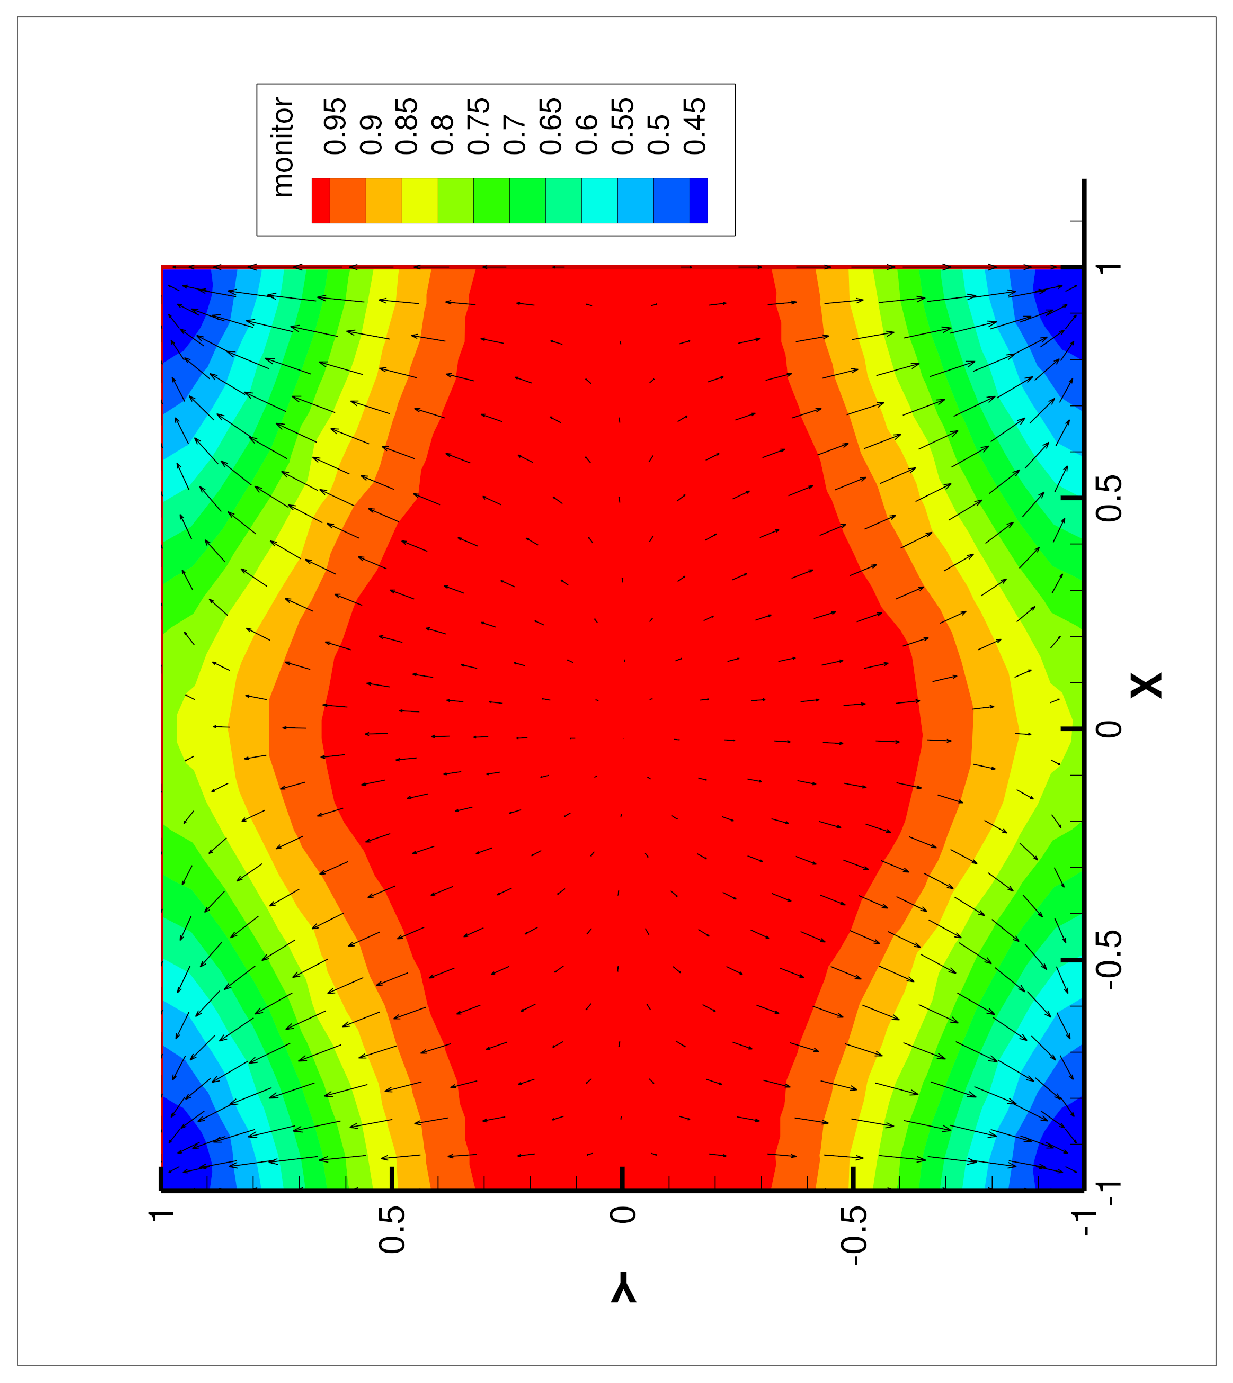
\includegraphics[width = 0.43\textwidth, angle = -90]{picture/first/collidingFlow/mesh_move_direction.eps}
              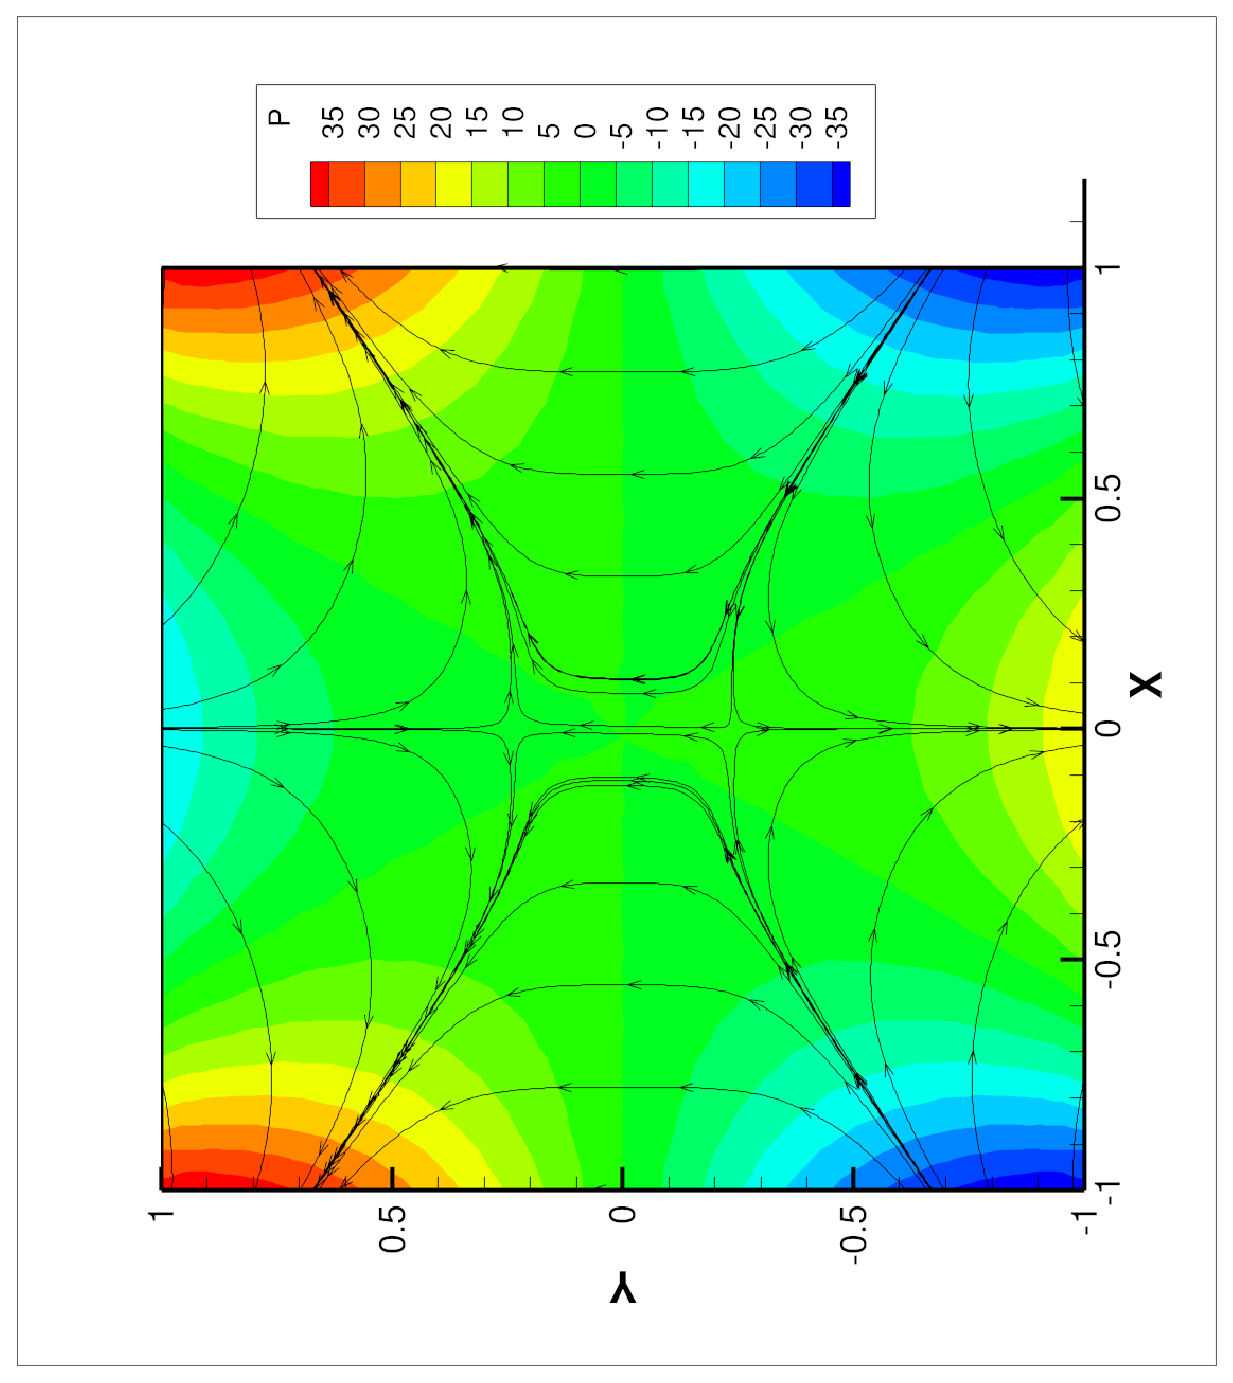
\includegraphics[width = 0.43\textwidth, angle = -90]{picture/first/collidingFlow/pressure_contour.eps}
              \caption{\small ��$m = \frac{1}{G_1}$�ĵȸ��ߺ�������
                �������ң�ѹ���ȸ��ߺ��ٶȵ������� $\alpha = 0.002, \beta = 2.0$.}
              \label{fig::mesh_move_direction}
            \end{center}
          \end{figure}

          \begin{figure}[ht]
            \begin{center}
              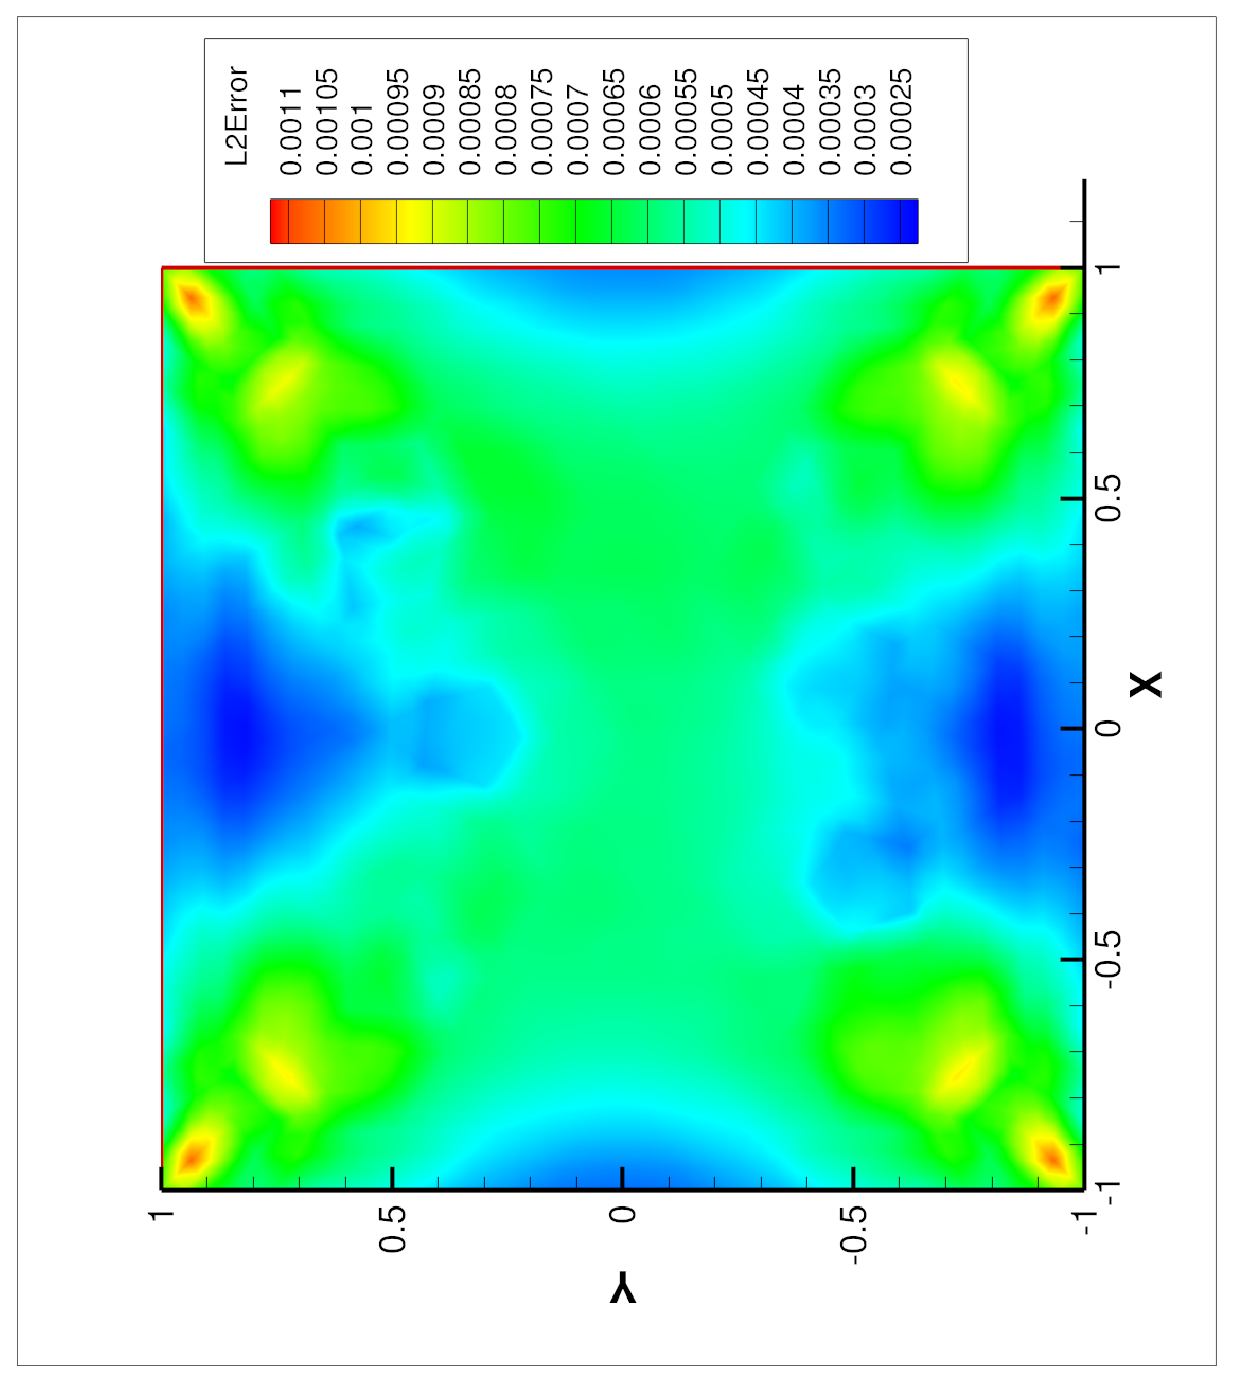
\includegraphics[width = 0.43\textwidth, angle = -90]{picture/first/collidingFlow/uniform20_error.eps}
              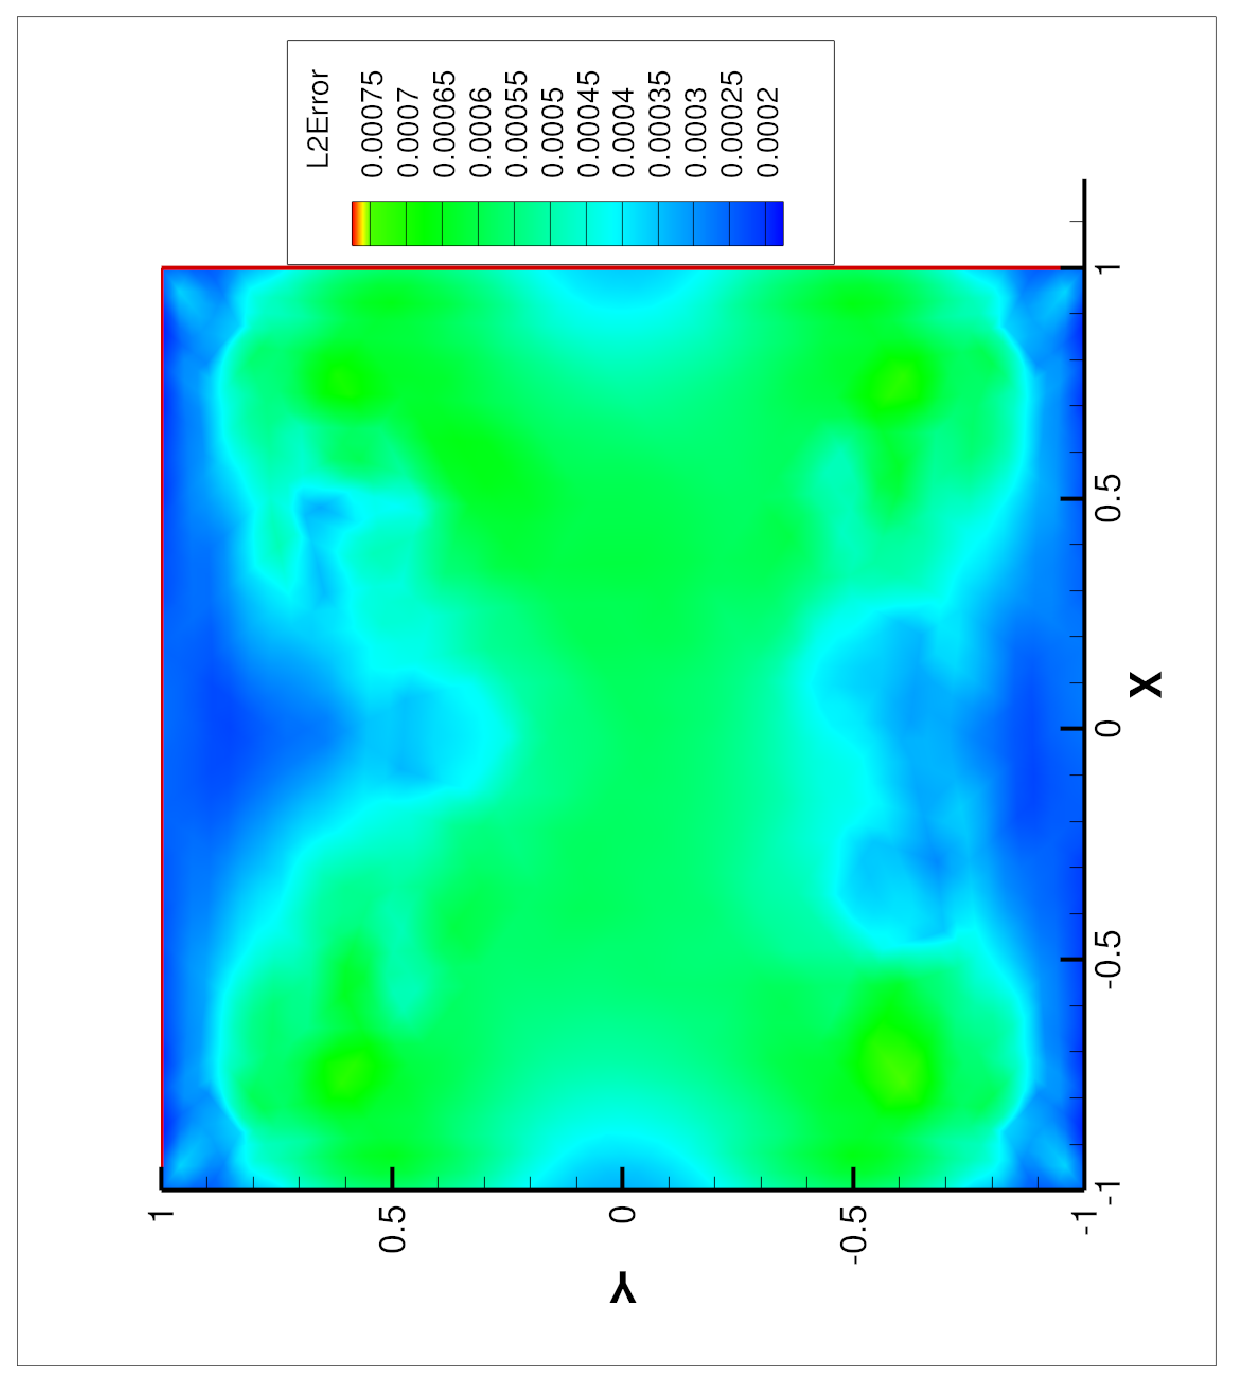
\includegraphics[width = 0.43\textwidth, angle = -90]{picture/first/collidingFlow/moving20_error.eps}
              \caption{\small �ٶ�$L^2$���ֲ����󣺾��������ң��ƶ����� $\alpha = 0.002, \beta = 2.0$.}
              \label{fig::uniform_vs_moving_err}
            \end{center}
          \end{figure}



          \begin{figure}[ht]
            \begin{center}
              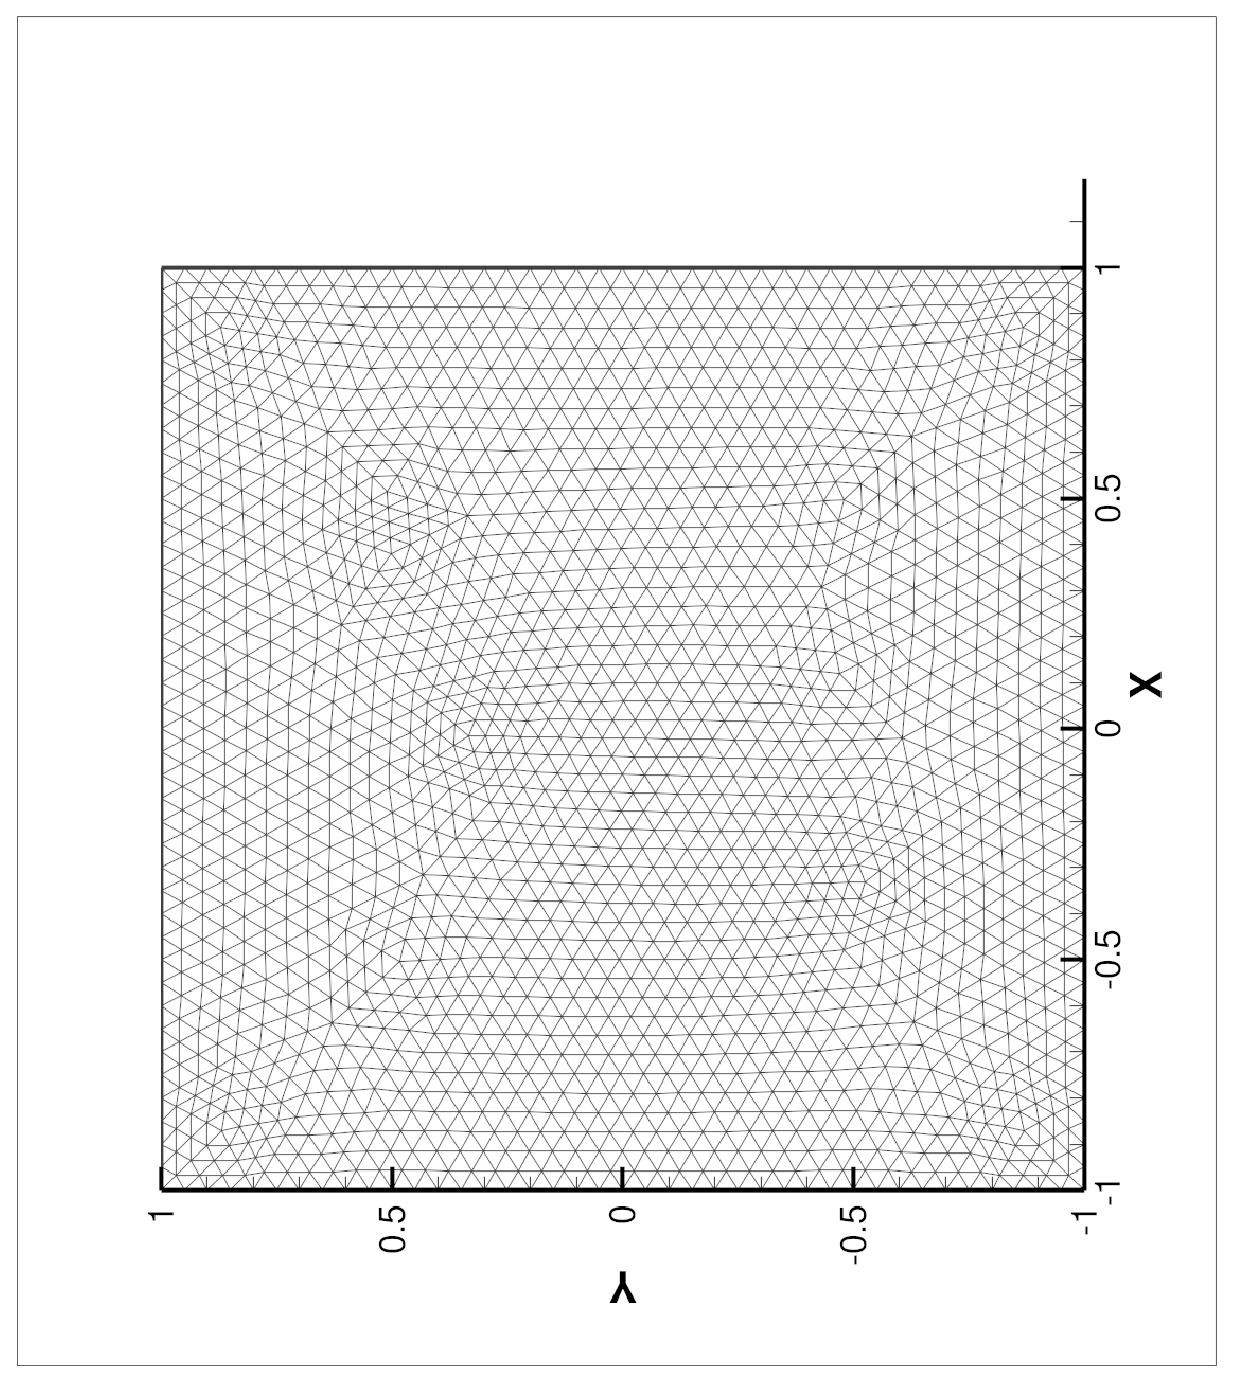
\includegraphics[width = 0.43\textwidth, angle = -90]{picture/first/collidingFlow/uniform_mesh20.eps}
              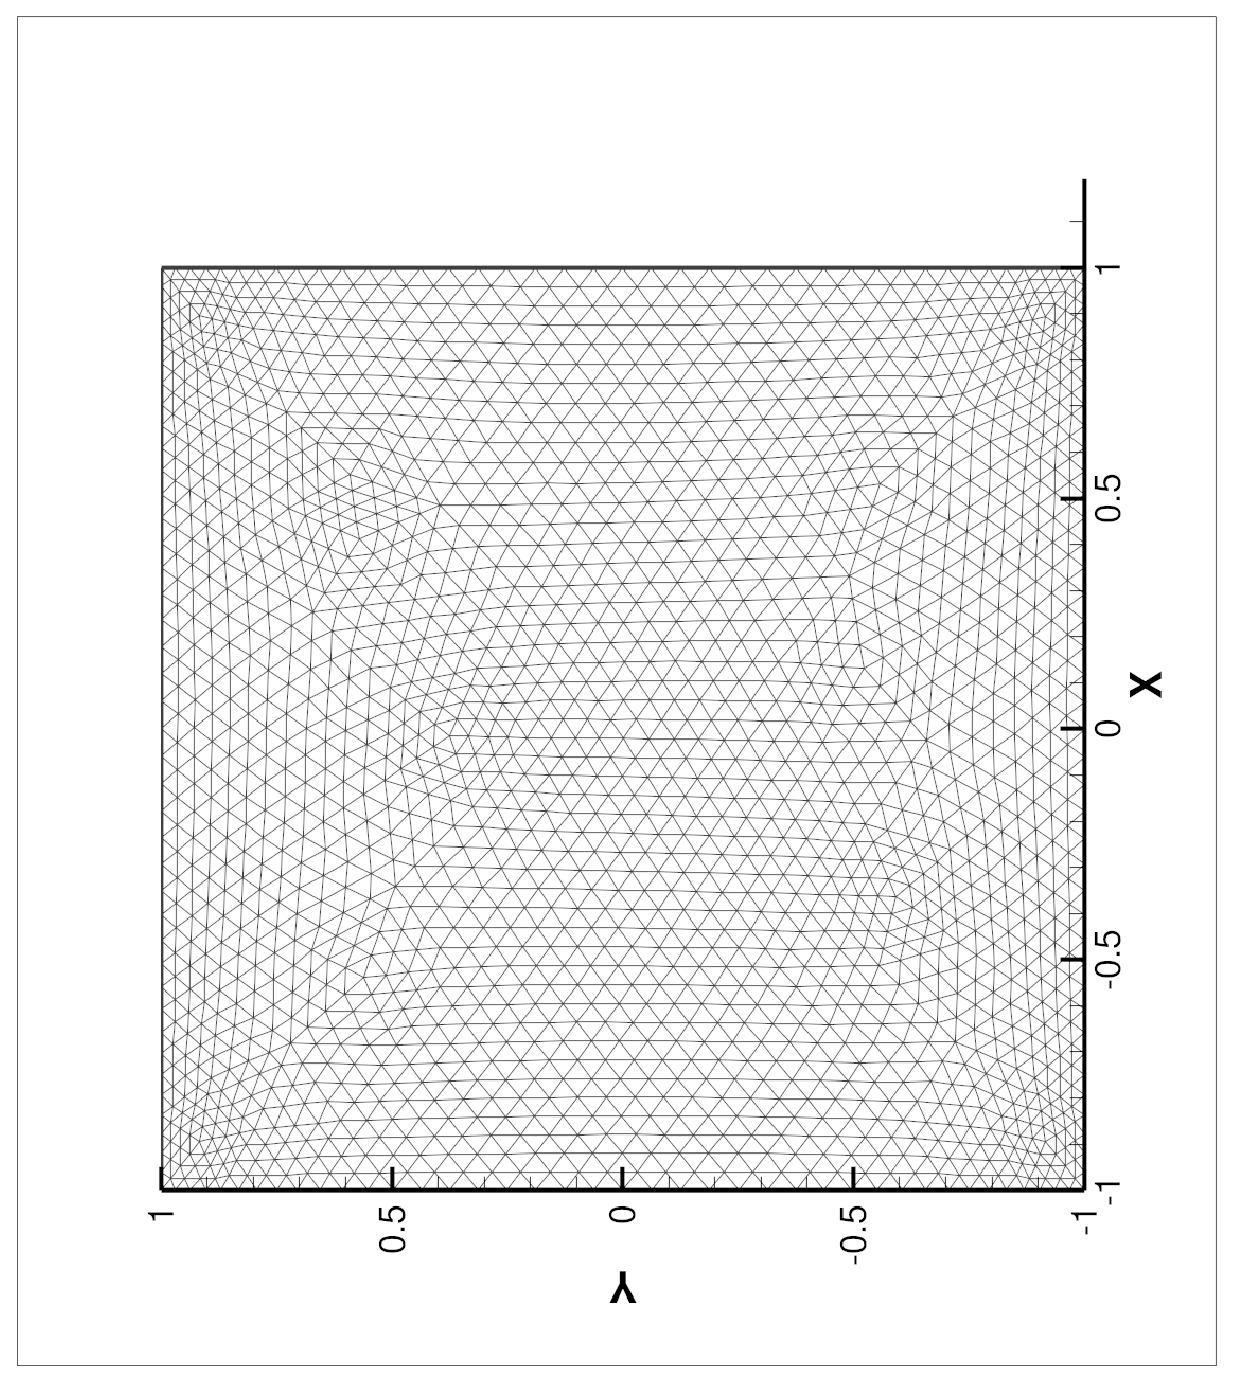
\includegraphics[width = 0.43\textwidth, angle = -90]{picture/first/collidingFlow/moving_mesh20.eps}
              \caption{\small ����Աȣ��󣺾�������$20 \times 20$���ң��ƶ����� $\alpha = 0.002, \beta = 2.0$.}
              \label{fig::uniform_vs_moving_mesh}
            \end{center}
          \end{figure}

     \subsection{������}

       �������ģ�����һ����ϸ������������һ����ֹ������������������Բο�\cite{milton1982album}, һ����Ȥ�Ļ��ᡣ
       ���ǵļ���������$\Omega = [0, 12] \times [-3, 3]$ ����ճ��ϵ����$\nu = 0.0005$����Ȼ���������ڳ����߽�$x = 12$�ϣ�
       ͬʱ������$x = 0, y \in [-0.1, 0.1]$������Poiseuille��������
       \begin{equation}
         u_x = 1 - 100 y^2, u_y = 0.
       \end{equation}
       �޻��Ʊ߽�����������$\partial \Omega$�����ಿ�֡�

       ���ƶ���������У�����ѡȡ (\ref{eq::monitor_vorticity})��Ϊ���ƺ���������$\alpha = 2.0, \beta = 2.0$��
       ��������֪����ϸ�����䵽��ֹ�������У�����������ԳƵ��С�Ϊ����߼��㾫�ȣ�����������Χ��Ҫ���������
       ��ͼ\ref{fig::jetting_flow_mesht12s}�п��Կ�����������������ֵ�Ƚϴ�ĵط�������ʱ��ķ�չ������IJ�
       �ȶ��������֣����\cite{milton1982album}�е�����������һ�µġ�
       \begin{figure}[!htbp]
         \begin{center}
             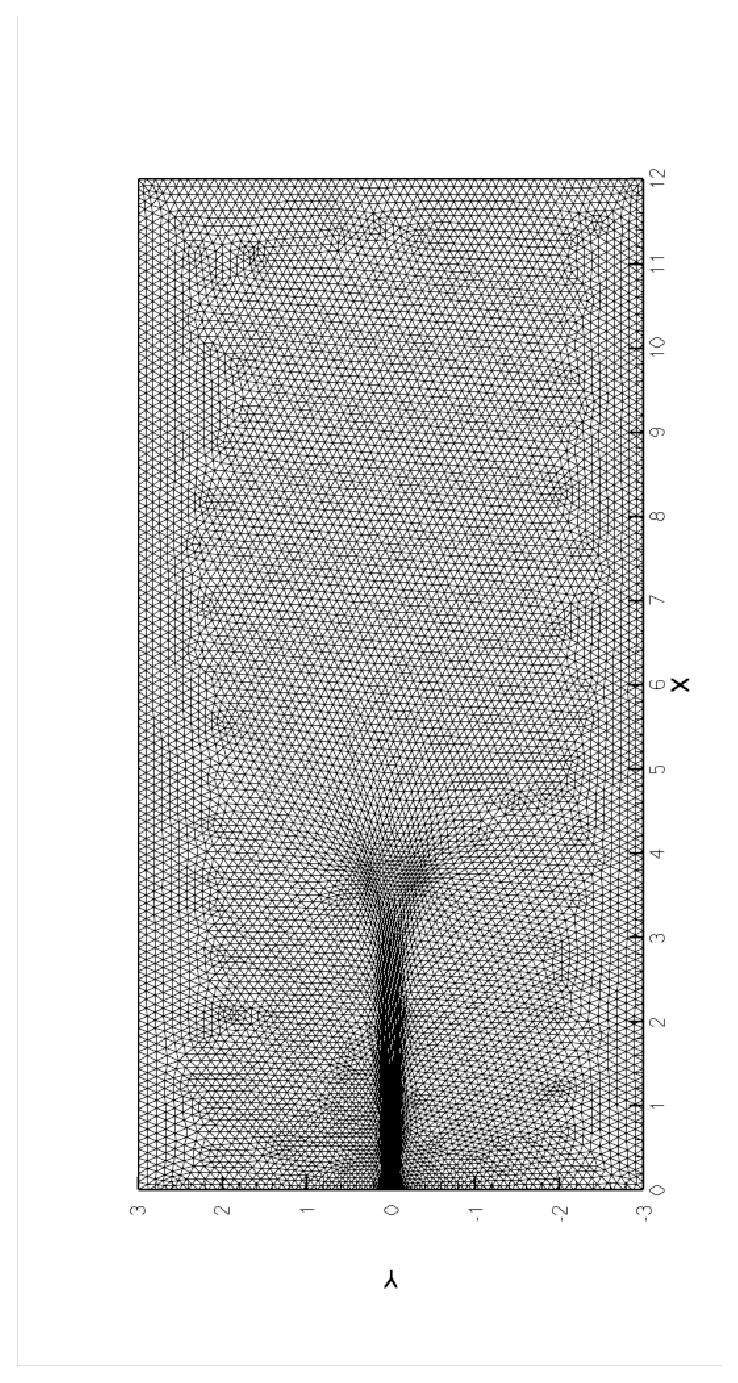
\includegraphics[width = 0.53\textwidth, angle = -90]{picture/first/jet_flow_data/mesh_t12s.eps}
             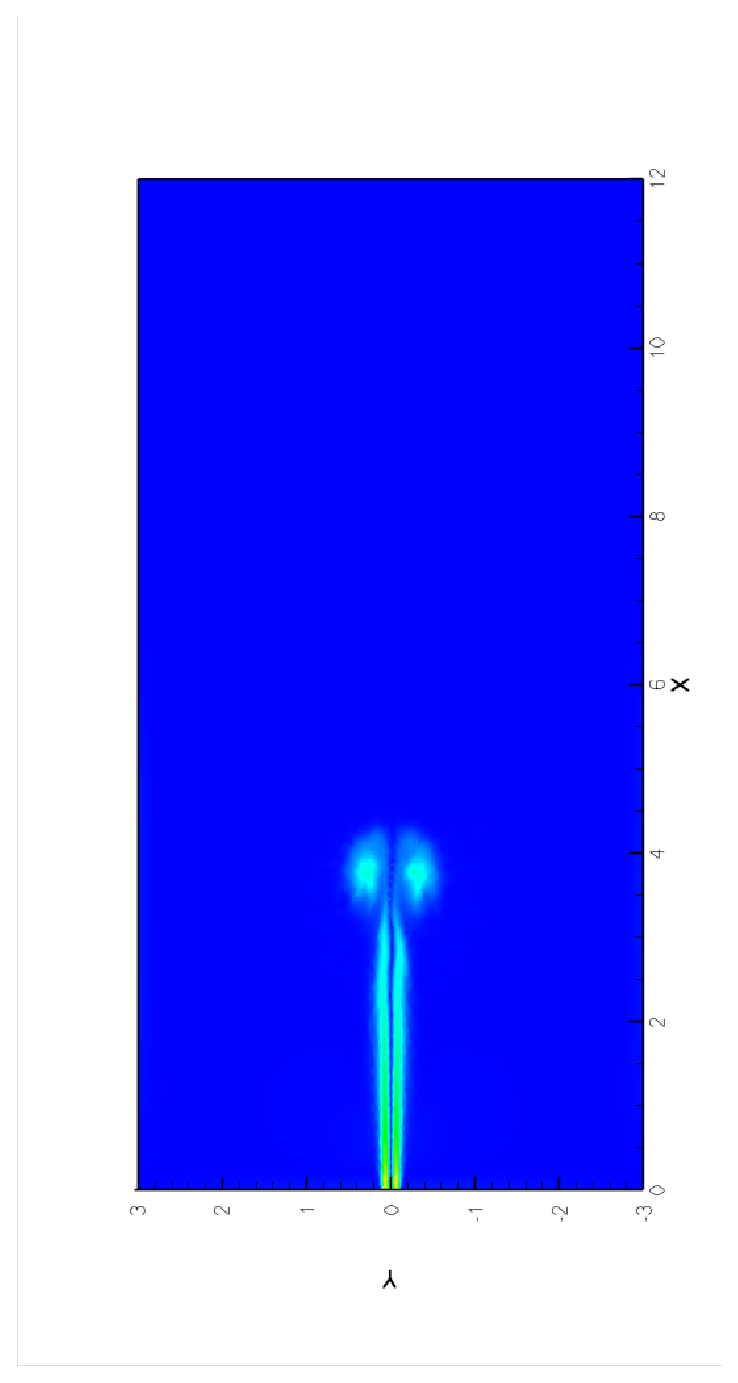
\includegraphics[width = 0.53\textwidth, angle = -90]{picture/first/jet_flow_data/contour_t12s.eps}
        \end{center}
        \caption{\small Jetting flow: top: mesh, bottom: vorticity contour at t = 12s.}
        \label{fig::jetting_flow_mesht12s}
       \end{figure}

       \begin{figure}[!htbp]
         \begin{center}
             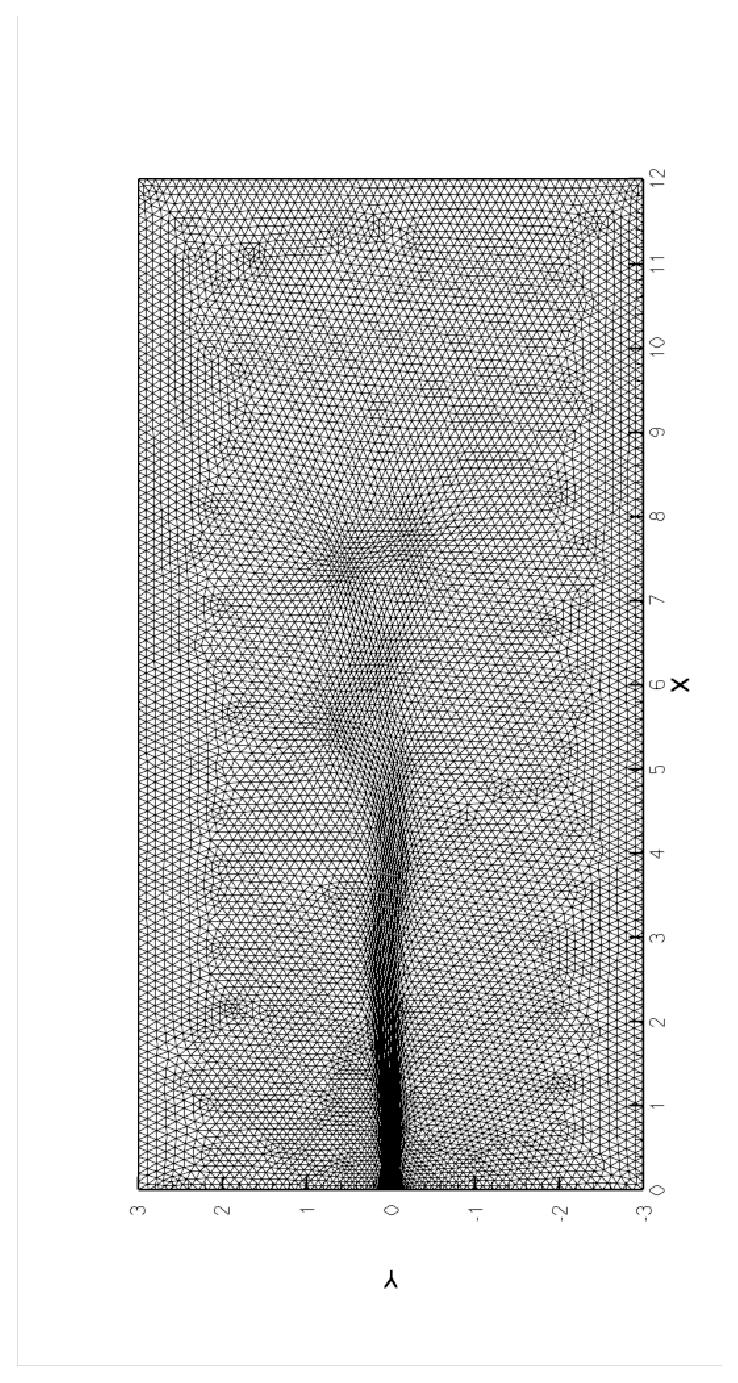
\includegraphics[width = 0.53\textwidth, angle = -90]{picture/first/jet_flow_data/mesh_t27s.eps}
             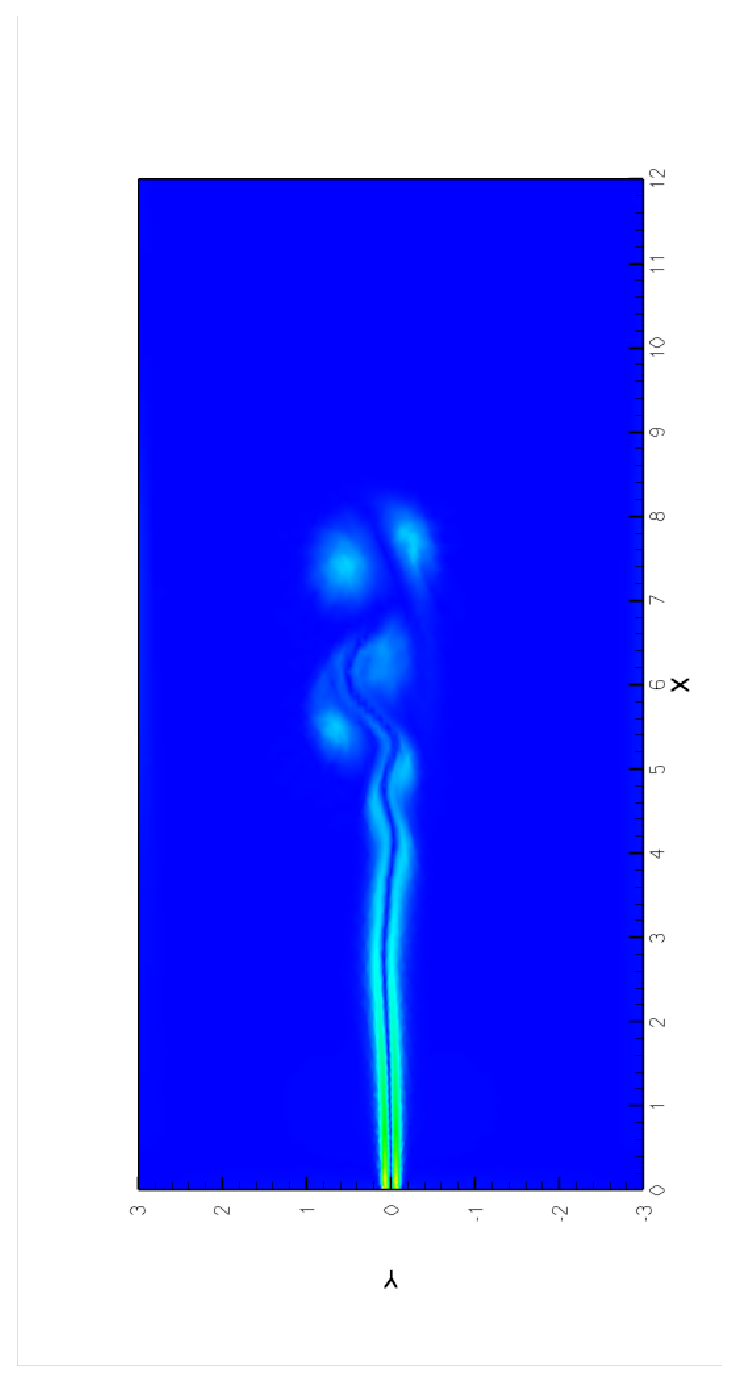
\includegraphics[width = 0.53\textwidth, angle = -90]{picture/first/jet_flow_data/contour_t27s.eps}
        \end{center}
        \caption{\small Jetting flow: top: mesh, bottom: vorticity contour at t = 27s.}
        \label{fig::jetting_flow_mesht27s}
       \end{figure}


   \subsection{Navier-Stokes ������һ������̨��}


      ���ǿ���\cite{zheng2010posteriori}�е�������Navier-Stokes ������$Re = 1000$����һ�����ε�̨�ף�����������
      $\Omega = (0, 4) \times (0, 1)/(1.2, 1.6) \times (0, 0.4)$�������±߽��ϣ�����$\vec{u} = (0, 0)^T$�ı߽�������
      �������ϵı߽�����Ϊ$\vec{u} = (4 y (1 - y), 0)$������������Ȼ�߽�������

      ����ѡȡ������Ϊ���ƺ��������ƺ����IJ����� $\alpha = 0.4, \beta = 2.0$��������֪������������������ڰ���ȥ�Ľ��ϣ�
      ����������ԡ���ͼ\ref{fig::step_initial_mesh}�п��Կ�������ʼ���������ڰ���ȥ�ı��ϡ�$t = 0.5s, t = 1s \text{, and } t = 2s$
      ʱ�̵������Լ������ĵȸ�����ͼ\ref{fig::step_flow_05s}��\ref{fig::step_flow_1s} �� \ref{fig::step_flow_2s}��չʾ��
      �������Ƿ��֣����ǵ�������еĽṹ��һ�µġ�

      $t = 2s$ʱ��ѹ���ĵȸ����Լ��ٶȵ���������ͼ\ref{fig::step_flow_contour_streamline_2s}�и��������ǿ��Կ������ڹսǴ���ѹ����
      �ȸ�����ƽ���ġ�

      \begin{figure}[!htbp]
        \begin{center}
        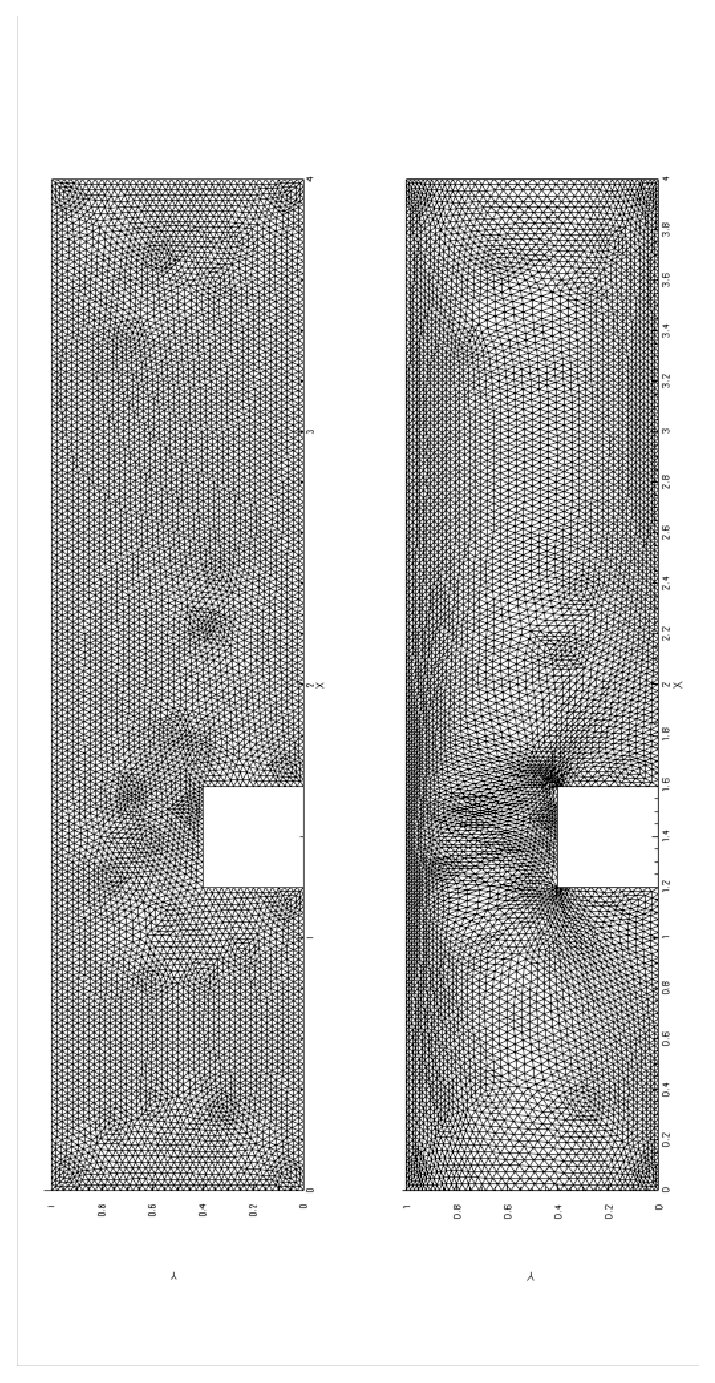
\includegraphics[width = 0.55\textwidth, angle = -90]{picture/first/step_flow_data/initial_mesh40_001.eps}
        \caption{\small Top: initial uniform mesh; bottom: initial moving mesh.}
        \label{fig::step_initial_mesh}
        \end{center}
      \end{figure}

      \begin{figure}[!htbp]
        \centering
        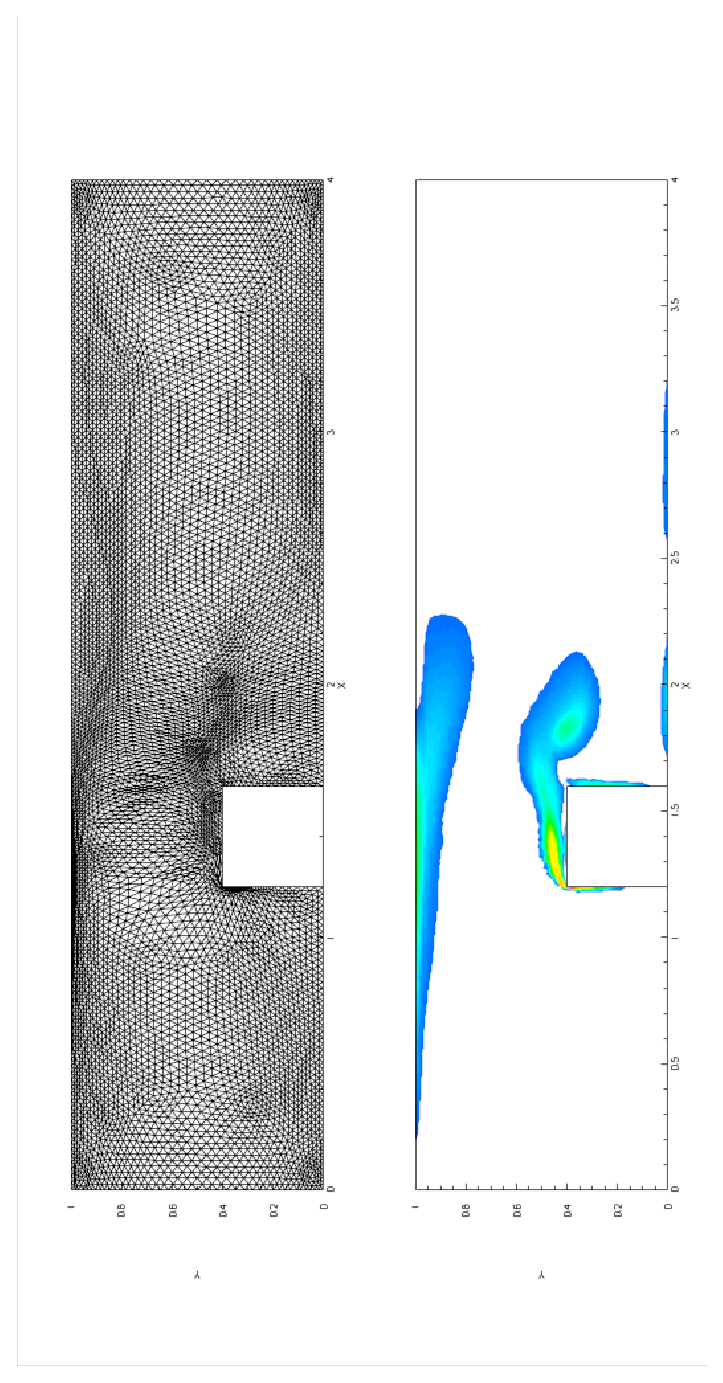
\includegraphics[width = 0.55\textwidth, angle = -90]{picture/first/step_flow_data/mesh_t_05.eps}
        \caption{\small Top: moving mesh; bottom: contour of vorticity
          at t = 0.5s}
        \label{fig::step_flow_05s}
      \end{figure}

      \begin{figure}[!htbp]
        \centering
        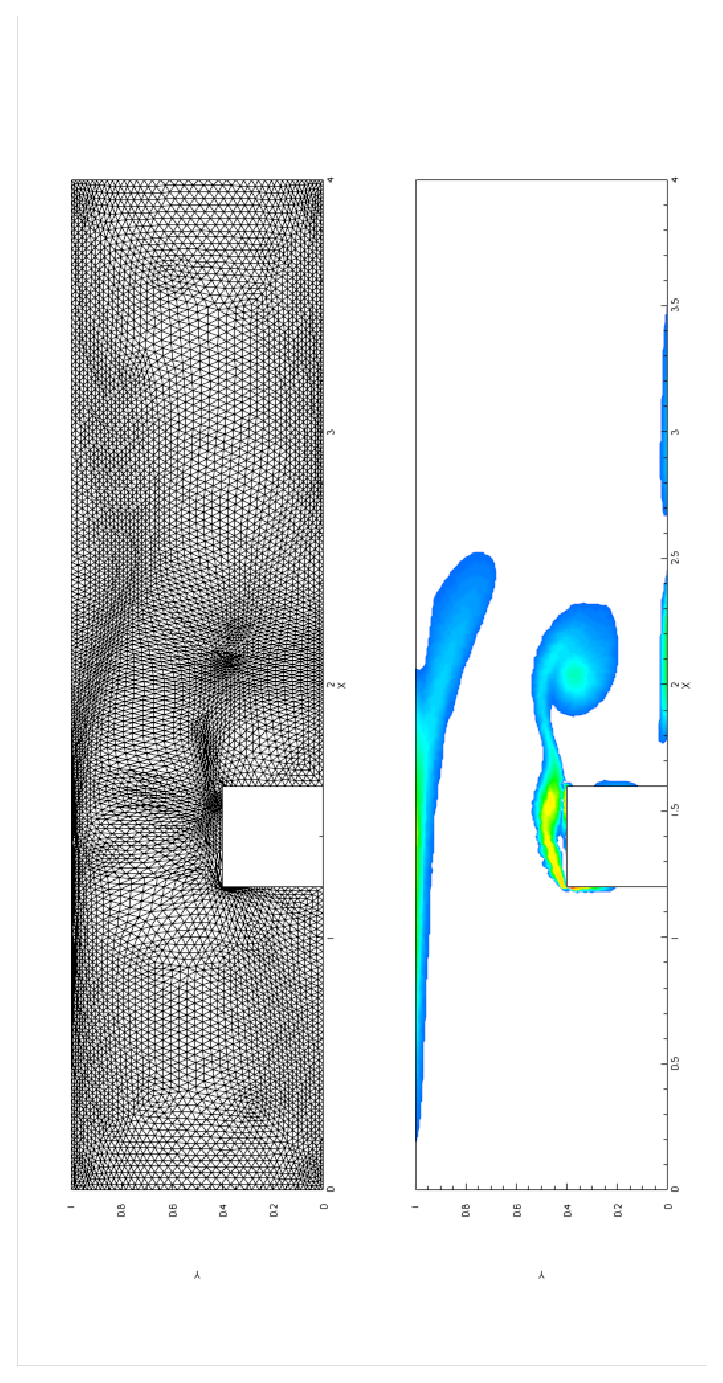
\includegraphics[width = 0.55\textwidth, angle = -90]{picture/first/step_flow_data/mesh_t_1s.eps}
        \caption{\small Top: moving mesh; bottom: contour of vorticity
          at t = 1s}
        \label{fig::step_flow_1s}
      \end{figure}

      \begin{figure}[!htbp]
        \centering
        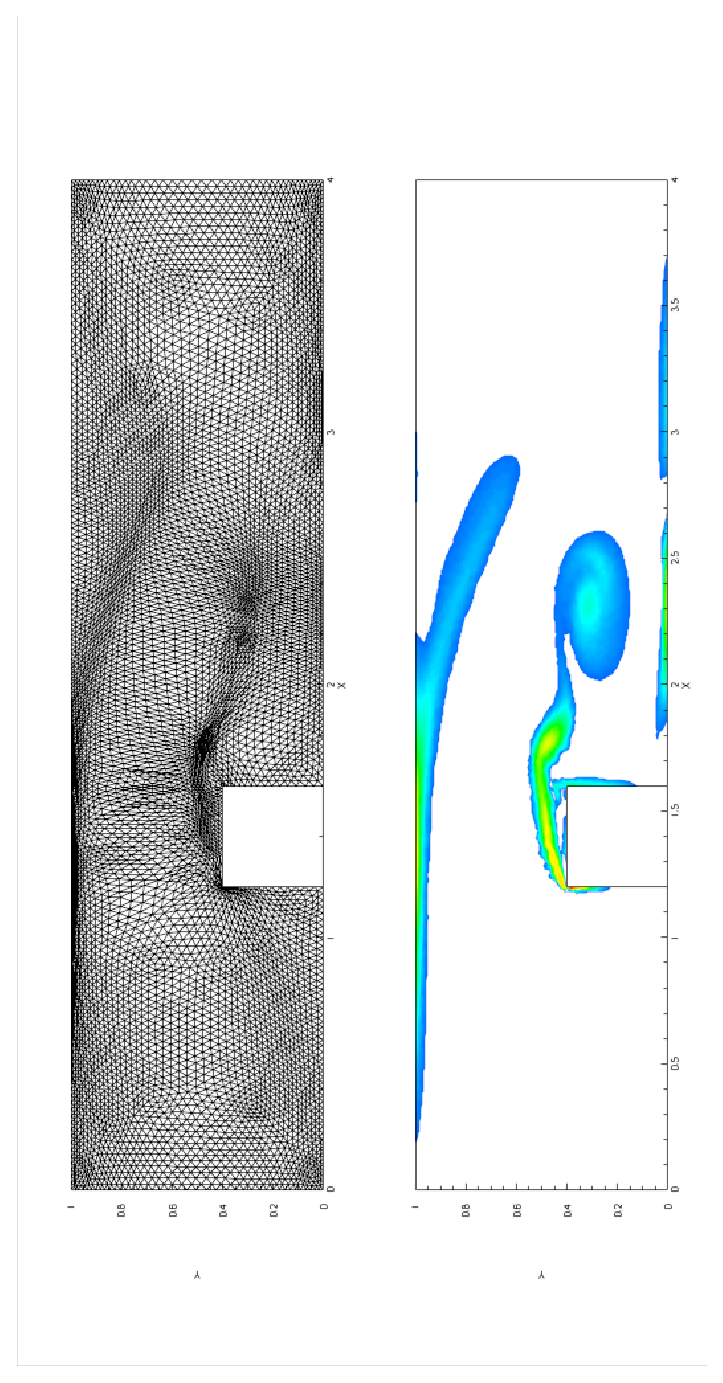
\includegraphics[width = 0.55\textwidth, angle = -90]{picture/first/step_flow_data/mesh_t_1_5s.eps}
        \caption{\small Top: moving mesh; bottom: contour of vorticity
          at t = 1.5s}
        \label{fig::step_flow_1_5s}
      \end{figure}

      \begin{figure}[!htbp]
        \centering
        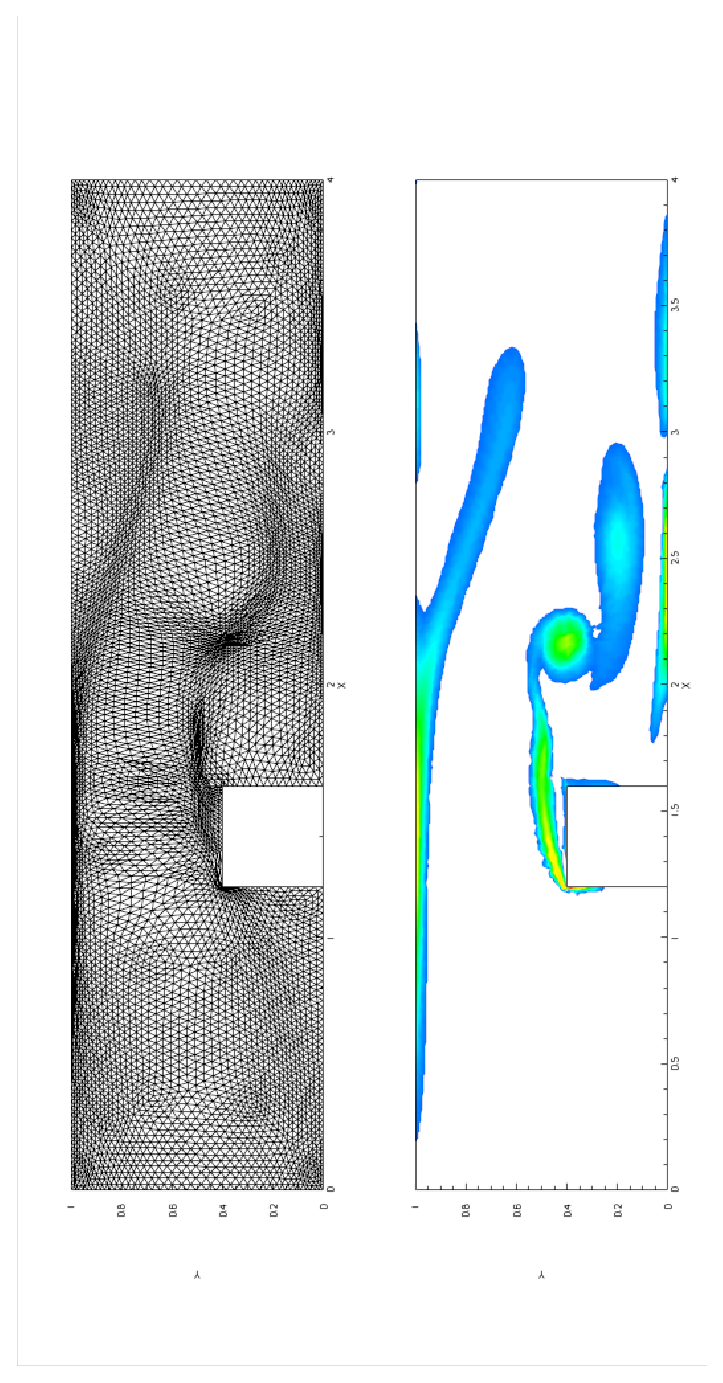
\includegraphics[width = 0.55\textwidth, angle = -90]{picture/first/step_flow_data/mesh_t_2s.eps}
        \caption{\small Top: moving mesh; bottom: contour of vorticity
          at t = 2s}
        \label{fig::step_flow_2s}
      \end{figure}

      \begin{figure}[!htbp]
        \centering
        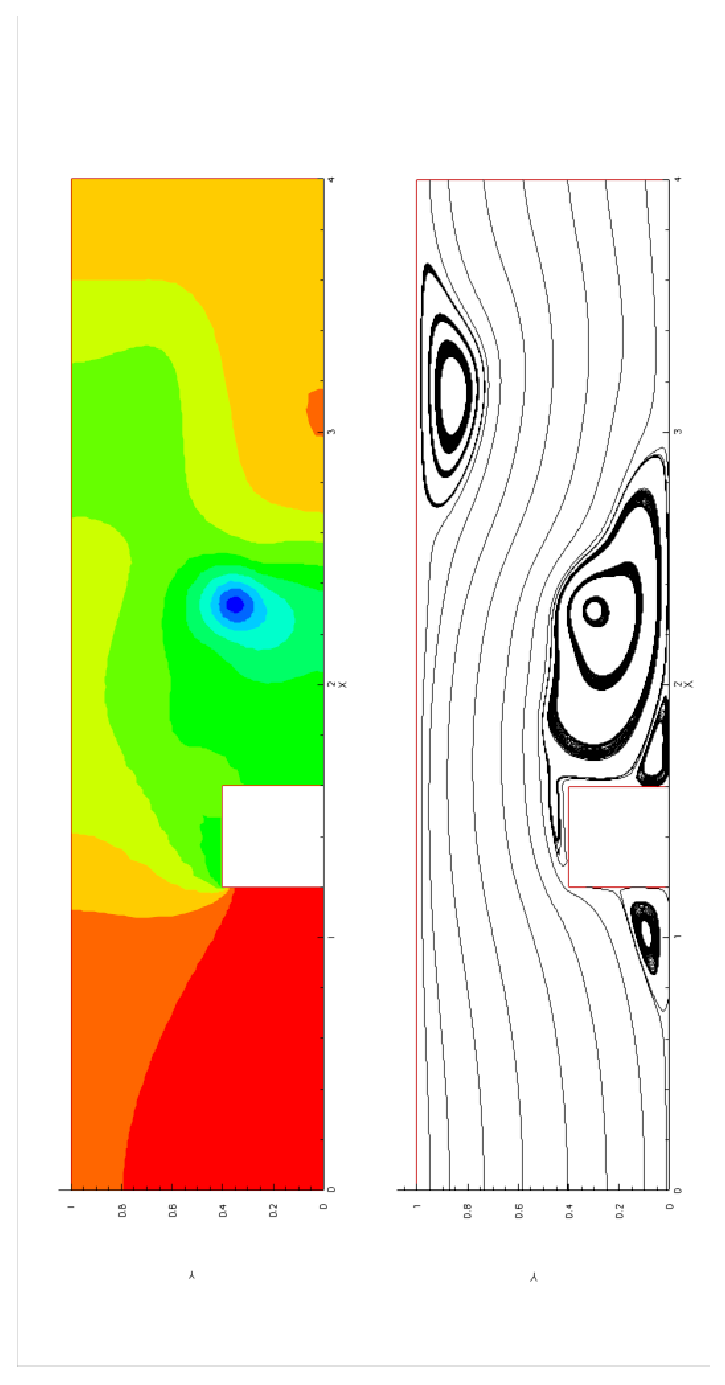
\includegraphics[width = 0.55\textwidth, angle = -90]{picture/first/step_flow_data/contour_streamline_t_2s.eps}
        \caption{\small Top: pressure contour; bottom: velocity streamline
          at t = 2s}
        \label{fig::step_flow_contour_streamline_2s}
      \end{figure}

   \subsection{Բ������}

      ����Ǿ�����������һ�������εĹܵ��У���������һ��Բ������\cite{cao1999anr}�У��������ƶ�����Ԫ������������
      ģ�͡�Բ��Բ����$(0, 0)$���뾶��$r = 0.3$��ճ��ϵ���� $\nu = 0.003$������������ $\Omega = [-1, 5] \times [-1, 1]$��
      Poiseuille�� $u = 1 - y^2, v = 0$ �����������߽� $x = -1$���߽����� $u = v = 0$ ʩ���ڹܵ������±߽硣�����߽� $x = 5$
      ����Ȼ�߽�������

      ������ǹ�ע�����ϸ΢�ṹ�������Ҫ��С�ṹ���и߷ֱ��ʡ�Ϊ��ץס�еĽṹ�������ǵ��ƶ������У�(\ref{eq::monitor_vorticity})
      ��Ϊ���ƺ�����һ���ܺõ�ѡ�񡣾���IJ����� $\alpha$ �� $\beta$ �ֱ�Ϊ $1.0$�� $2.0$��

      ��ͼ\ref{fig::cylinder_initial_mesh} �� ͼ \ref{fig::cylinder_mesh_t24_5s} �У�չʾ��������еĵȸ��ߵı仯�����п��Կ�����
      ���ǵ��������ץס�еĽṹ���������ǵ����������� \cite{cao1999anr}��Ҫ�á�
      �����Ǹı���ŵ��Ϊ $Re = 2000$ ʱ����ͼ\ref{fig::cylinder_mesh_t23s}�п��Կ���������������Ľṹ������ $Re = 2000/3$ ʱ��ô���ԡ�

      \begin{figure}[!htbp]
        \centering
        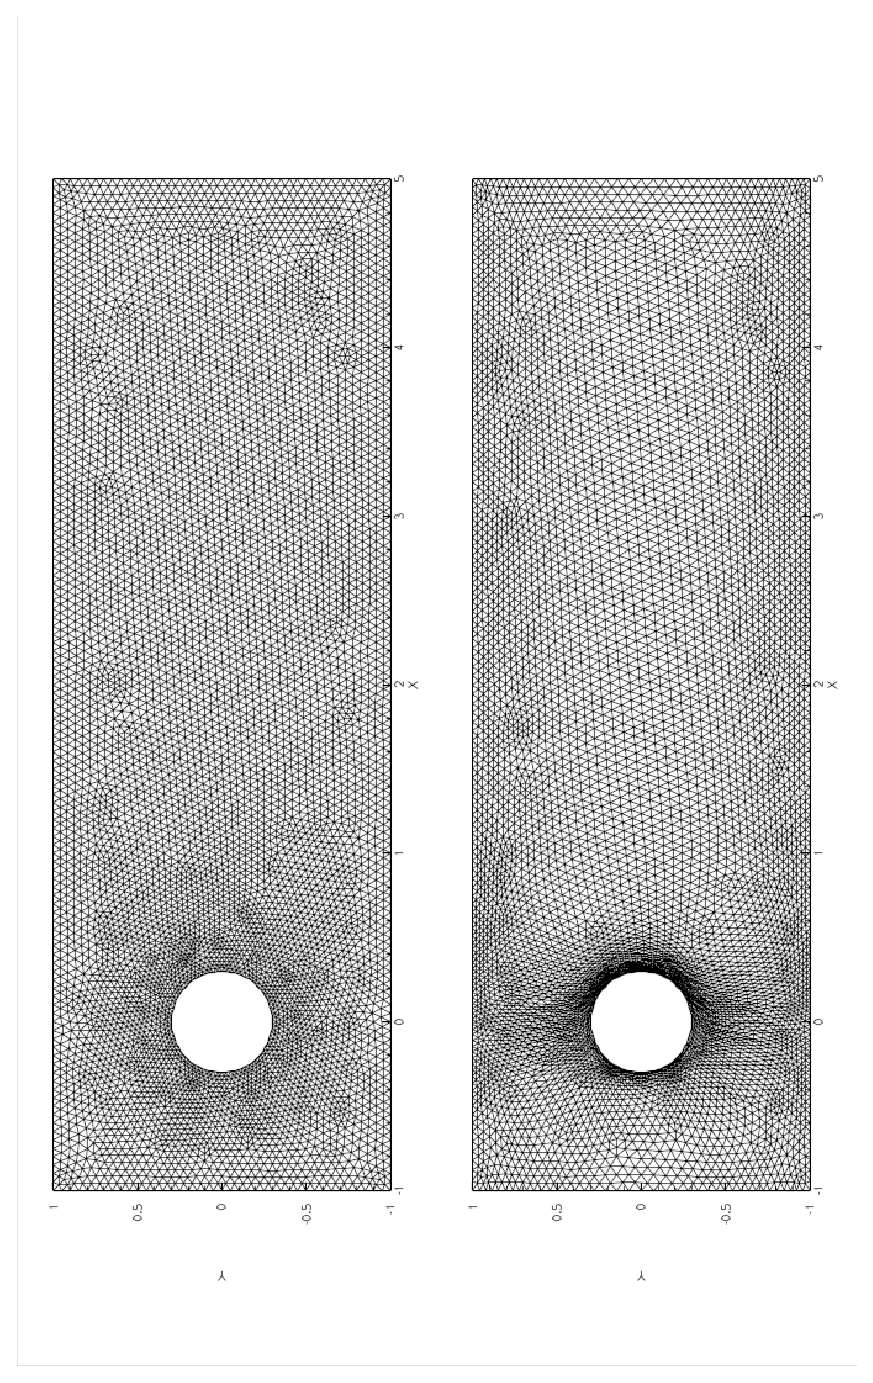
\includegraphics[width = 0.6\textwidth, angle = -90]{picture/first/obstacle_flow_data/initial_mesh.eps}
        \caption{\small Top: uniform mesh; bottom: initial
          moving mesh, viscosity $\nu = 0.003$.}
        \label{fig::cylinder_initial_mesh}
      \end{figure}

      \begin{figure}[!htbp]
       \begin{center}
         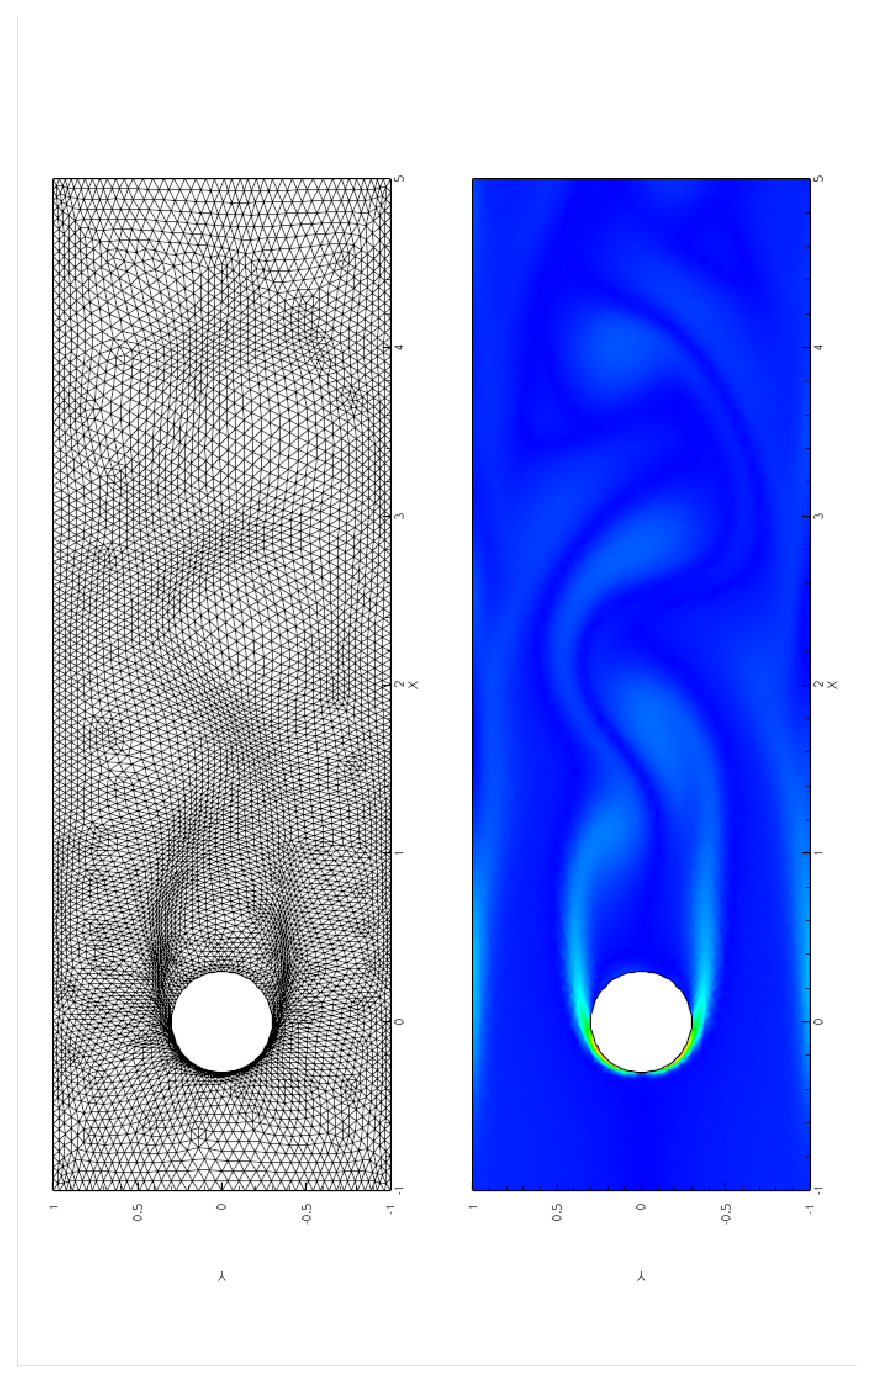
\includegraphics[width = 0.6\textwidth, angle = -90]{picture/first/obstacle_flow_data/mesh_t_24_5s.eps}
       \end{center}
       \caption{\small Top: moving mesh; bottom: vorticity contour at
         $t = 24.5s$, viscosity $\nu = 0.003$.}
       \label{fig::cylinder_mesh_t24_5s}
     \end{figure}

     \begin{figure}[!htbp]
       \centering
       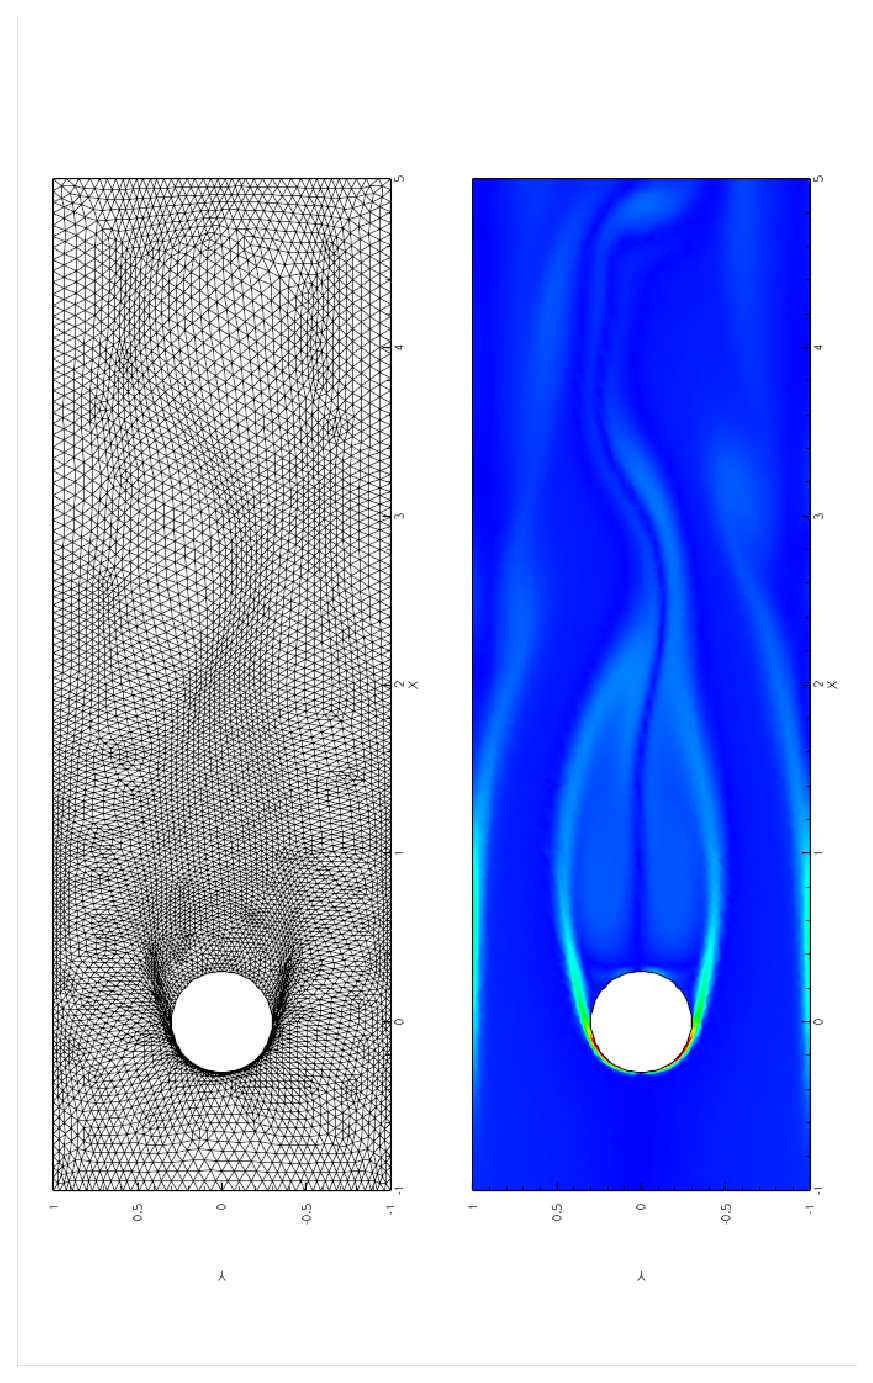
\includegraphics[width = 0.6\textwidth, angle = -90]{picture/first/obstacle_flow_data/mesh_t_23s.eps}
       \caption{\small Top: moving mesh; bottom: vorticity contour at
         $t = 23s$, viscosity $\nu = 0.001$.}
       \label{fig::cylinder_mesh_t23s}
     \end{figure}



\begin{numcases}{}
|r(E(z),\lambda)| < |r(z,\lambda)|^3, &
if \ $r(z,\lambda) \in \overline{\MCD}_1\backslash\{0,1\}$,\ \ \  \label{ineq:abs_r(E(z))_1}\\
|r(E(z),\lambda)| \leq \sup_{m \geq
3}\left\{\left|\frac{S_m(u)}{u^3}\right|\right\}\cdot \frac{|u| +
|r(z,\lambda)|}{|u| - |r(z,\lambda)|} \cdot |r(z,\lambda)|^3,  & if
\  $r(z,\lambda) \in \mathcal {D}_0\backslash\{1\}$,
\label{ineq:abs_r(E(z))_2}
\end{numcases}



\begin{table}[h]
\begin{center}
\begin{tabular}{cc@{\hspace{0.7cm}}c@{\hspace{0.7cm}}c@{\hspace{0.7cm}}c@{\hspace{0.7cm}}c@{\hspace{0.7cm}}c}
\hline
& Algorithm & CPU time (s)& iter & $k_1$ & $\rho(X)$ & err($X$) \\
\hline
$A_1^{1/5}$ \\
& PSN & 3.91e-03 & 5 & 2 & 1.75e-15 & 2.05e-15 \\
& SN & 3.28e-03 & 6 & 2 & 4.67e-16 & 1.05e-15 \\
& SH & 3.13e-03 & 3 & 2 & 6.15e-16 & 9.63e-16 \\
& SE & 3.59e-03 & 3 & 3 & 8.77e-16 & 1.55e-15 \\
$A_2^{1/15}$ \\
& PSN & 6.09e-03 & 5 & 5 & 1.48e-15 & 2.67e-08 \\
& SN & 5.17e-03 & 6 & 4 & 5.74e-15 & 2.67e-08 \\
& SH & 5.00e-03 & 3 & 4 & 7.82e-15 & 2.67e-08 \\
& SE & 4.53e-03 & 5 & 5 & 2.25e-14 & 2.67e-08 \\

\hline
\end{tabular}
\end{center}
\caption{Results for computing $A_1^{1/5}$ and $A_2^{1/15}$ by using
the four Algorithms. } \label{tab:test3}
\end{table}




  %%---------------------------------------------------------------------------%%
%%------------ 第四章:代数~Riccati~方程的~ULM~方法 ---------------------------%%
%%---------------------------------------------------------------------------%%


\chapter{移动网格有限元的多重网格预处理方法}
    \label{chapter:AMG_preconditioner}
    原始变量形式的不可压Navier-Stokes方程
    \begin{equation}
      \begin{array}{rcl}
         \partial_t \vec{u} - \nu \nabla^2 \vec{u} +
        (\vec{u} \cdot \nabla )\vec{u} + \nabla p & =
        & \vec{f},\\
        \nabla \cdot \vec{u} & = & 0,
      \end{array}
      \label{eq::NS}
    \end{equation}
    $\partial \Omega = \partial \Omega_D \bigcup \partial \Omega_N$上的
    边界条件以及初值条件:
    \begin{equation}
      \begin{array}{ll}
        \vec{u} = \vec{w},& \mbox{ on } \partial \Omega_D \times [0,
        T]\\
        \nu \displaystyle \frac{\partial \vec{u}}{\partial n} - p =
        \vec{0}, & \mbox{ on } \partial \Omega_N \times [0, T],  \\
        \vec{u}|_{t = 0} = \vec{u_0}, & \mbox{ in } \Omega.
      \end{array}
      \label{eq::bc}
    \end{equation}
    其中 $\Omega \in \mathcal{R}^d,(d = 2, 3)$ 是计算区域,
    $[0,T]$ 是时间区间, $\vec{u}$是速度变量并且常量$p$是压力, $\vec{n}$ 是边界
    $\partial \Omega$上的外法向方向, $\nu > 0$ 是粘性动力学系数。
    我们用\cite{li2001mesh} 和 \cite{di2005}中提出的移动网格有限元方法求解(\ref{eq::NS}) 和 (\ref{eq::bc})。
    过去几十年,很多人在移动网格移动网格方法上做出了很多工作(\cite{cao1999adaptive}、
    \cite{cao2003moving}、\cite{di2005moving}、\cite{di2007level}、\cite{di2007moving}、
    \cite{li2001PHDthesis}、\cite{li2006moving})。Winslow \cite{Winslow1966NUMERICAL} 提出了
    用移动网格方法求解椭圆方程。作为Winslow的工作的拓展, Dvinsky \cite{dvinsky1991adaptive}
    提出了调和函数理论可以用来产生网格。收到Dvinsky工作的启发, L1, Tang and Zhang \cite{li2001mesh}
    提出了基于调和映射的移动网格有限元方法。邸\cite{di2005moving}把这种移动网格策略应用到求解原始
    变量形式的不可压Navier-Stokes方程。文中在移动网格策略中提出了保持散度的插值方法,这是通过
    求解一个类似线性化的Navier-Stokes方程。我们在上一章中,提到了我们将$4P1-P1$元应用到移动网格    有限元方法上。$4P1-P1$元自然满足LBB(inf-sup)条件,在\cite{bercovier1979error}给出了$P1isop2P1$
    元的误差收敛阶,速度$L^2$误差是二阶收敛,压力是一阶收敛。$4P1-P1$跟$P1isoP2P1$元具有相同的
    数据结构,但是$4P1-P1$元中的速度单元上的基函数全部位于一个速度单元上,在速度单元和压力单元
    进行拼装的时候,只要建立速度单元和压力单元间的索引,便是一个简单的过程。

    据我们所知,用满足inf-sup条件的$4P1-P1$元可以推出一个鞍点问题,许和何(\cite{xu1992iterative}、\cite{shen1999schur}、\cite{he2003})
    将两格子方法应用到Navier-Stokes方程的求解。很多人在为krylov子空间方法提供预处理子方面做出了很多工作。
    在\cite{benzi2005numerical}文中,概括了求解鞍点问题常用的数值方法,例如块预处理和多重网格预处理。文献(
    \cite{bai2005inexact}, \cite{bai2006structured},\cite{elman2007least},\cite{elman2009boundary}等)中提出了许多块预处理方法,来
    找到鞍点问题的schur补的更好的近似。\cite{benzi2006augmented}中提出了求解Ossen系统的增广的基于lagarian方法。在\cite{benzi2011relaxed}
    中提出了求解不可压Navier-Stokes方程的维数分解的预处理方法。(\cite{boyle2007hsl}
    \cite{boyle2010hsl_mi20})中提出了求解Navier-Stokes方程的一种高效的Krylov子空间方法,这种方法是用代数多重网格做预处理子。
    但是据我们所知,对于鞍点问题的高效预处理方法基本上都是基于均匀网格上的,尽管在\cite{benzi2011relaxed}一文中,考虑了拉伸
    网格的情形。

    在\cite{elman2005finite}的基础上,我们将为移动网格有限元方法求解(\ref{eq::NS})和
    (\ref{eq::bc})提供了一个代数多重网格预处理方法。我们通过数值例子来表明,我们的预处理子的高效性。
    \section{时间格式的离散}
        在时间层离散上,我们把时间区间$[0, T]$分成$N$份,$\{t_i\}_{i = 1}^N$。令$\vec{u}^j$ 和 $p^j$ 是连续形式解$\vec{u}(\cdot, t_j)$ 和 $p(\cdot, t_j)$的离散近似。在时间格式的离散上,主要分为算子分裂方法和全隐格式。
        在算子分裂方法,也可以看成是分部方法。最简单的方法是将算子分成两步,在每一步中分别用向前和向后欧拉格式,可以参考\cite{peaceman1955numerical}。
        在\cite{he2003two}中,将这种两步分裂方法应用到Navier-Stokes方程的时间离散上。
        通常的两步方法如下:
        \begin{algorithm}
            \caption{Peaceman-Rachford 格式}
            \begin{algorithmic}[1]
                给定$\vec{u}^0, p^0, \theta \in [0, 1], \alpha \in (0, 1) \beta \in (0, 1)$, 假设$\vec{u}^n$已知,通过以下求解$\vec{u}^{n + 1}$:
                \begin{eqnarray}
                    \begin{aligned}
                        \frac{\vec{u}^{n + \theta} - \vec{u}^n}{\theta \delta t} - \alpha \nu \nabla^2\vec{u}^{n + \theta} + \vec{u}^* \cdot \nabla\vec{u}^{n + \theta}
                        & = \beta \nu \nabla^2\vec{u}^n - \nabla p^n \quad \mbox {在} \Omega \mbox{内},& \\
                        \vec{u}^{n + \theta} & = \vec{g}^{n + \theta} \quad \mbox{在} \partial \Omega \mbox{上}:&                                 \label{eq::first_step_PR}
                    \end{aligned}
               \end{eqnarray}
               \begin{eqnarray}
                    \begin{aligned}
                        \frac{\vec{u}^{n + 1} - \vec{u}^{N + \theta}}{(1 - \theta)\delta t} - \beta \nu \nabla^2\vec{u}^{n + 1} + \nabla p^{n + 1}
                        & =  \alpha \nu \nabla^2 \vec{u}^{n + \theta} - \vec{u}^* - \nabla \vec{u}^{n + \theta} \quad \mbox{在} \Omega \mbox{内},&\\
                        \nabla \cdot \vec{u}^{n + 1} & =  0 \quad \mbox{在} \Omega \mbox{内},&\\
                        \vec{u}^{n + 1} & = \vec{g}^{n + 1} \quad \mbox{在} \partial \Omega 上.&
                        \label{eq::second_step_PR}
                    \end{aligned}
               \end{eqnarray}
            \end{algorithmic}
            \label{alg::Peaceman_Rachford}
         \end{algorithm}
         在(\ref{alg::Peaceman_Rachford})中$\vec{u}^*$的取值要保证散度为0的条件,并且$\alpha + \beta = 1$。它实际上是先求解一个对流方程
         (\ref{eq::first_step_PR}),然后再求解一个广义的Stokes方程(\ref{eq::second_step_PR})。这个算法第一步计算的时候需要$p^0$的值,它
         可以在很小的时间步长情况下,全隐格式向前发展一步得到。一般自然的,$\vec{u}^* = \vec{u}^n$, 这样在时间格式上只有一阶精度的。这种
         方法不是无条件稳定的,并且需要比较小的时间步长。当$\theta = \frac{1}{2}, \vec{u}^* = \vec{u}^{n + theta}$时,可以获得二阶精度,
         这时候求解(\ref{eq::first_step_PR})变成了一个求解非线性的对流方程。详细内容可以参考(\cite{silvester1996fast})。\cite{dean1993some}将
         两步Peaceman-Rachford推广到三步, 保持了当$t \leftarrow \infty$时的数值稳定性:
         \begin{algorithm}
             \caption{Glowinski $\Theta$格式}
            \begin{algorithmic}[1]
                给定$\vec{u}^0, \theta \in [0, 1/2], \alpha \in (0, 1), \beta \in (0, 1)$, 假设$\vec{u}^n$已知,通过以下求解$\vec{u}^{n + 1}$:
                \begin{eqnarray}
                    \begin{aligned}
                        \frac{\vec{u}^{n + \theta} - \vec{u}^n}{\theta \delta t} - \alpha \nu \nabla^2\vec{u}^{n + \theta} +
                        \nabla p^{n + \theta}
                        & = \beta \nu \nabla^2\vec{u}^n - \vec{u}^n \cdot \nabla\vec{u}^{n} \quad \mbox {在} \Omega \mbox{内},& \\
                        \nabla \cdot \vec{u}^{n + \theta} & =  0 \quad \mbox{在} \Omega \mbox{内},&\\
                        \vec{u}^{n + \theta} & = \vec{g}^{n + \theta} \quad \mbox{在} \partial \Omega \mbox{上};& \\
                    \end{aligned}
                    \label{eq::first_step_GL_theta}
                \end{eqnarray}
                \begin{eqnarray}
                    \begin{aligned}
                        \frac{\vec{u}^{n + 1 - \theta} - \vec{u}^{n + \theta}}{(1 - 2\theta) \delta t} - \beta \nu \nabla^2\vec{u}^{n + 1 - \theta} + \vec{u}^* \cdot \nabla \vec{u}^{n + 1 -\theta}
                        & = \alpha \nu \nabla^2\vec{u}^{n + \theta}- \nabla p^{n + \theta} \cdot \nabla\vec{u}^{n} \quad \mbox {在} \Omega \mbox{内},& \\
                        \vec{u}^{n + 1 - \theta} & = \vec{g}^{n + 1 - \theta} \quad \mbox{在} \partial \Omega \mbox{上};& \\
                    \end{aligned}
                    \label{eq::second_step_GL_theta}
                \end{eqnarray}
                \begin{eqnarray}
                    \begin{aligned}
                        \frac{\vec{u}^{n + 1} - \vec{u}^{n + 1 - \theta}}{\theta \delta t} - \alpha \nu \nabla^2\vec{u}^{n + 1} +
                        \nabla p^{n + 1}
                        & = \beta \nu \nabla^2\vec{u}^{n + 1 - \theta} - \vec{u}^* \cdot \nabla\vec{u}^{n + 1 - \theta} \quad \mbox {在} \Omega \mbox{内},& \\
                        \nabla \cdot \vec{u}^{n + 1} & = 0 \quad \mbox{在} \Omega \mbox{内},&\\
                        \vec{u}^{n + \theta} & = \vec{g}^{n + \theta} \quad \mbox{在} \partial \Omega \mbox{上}.& \\
                    \end{aligned}
                    \label{eq::third_step_GL_theta}
                \end{eqnarray}
            \end{algorithmic}
         \end{algorithm}
         这种算法需要在每个时间步中计算两个广义的Stokes方程(\ref{eq::second_step_GL_theta}) 和(\ref{eq::third_step_GL_theta}), 和一个非线性的对流
         方程(\ref{eq::first_step_GL_theta})。当我们取$\alpha = \beta = 1/2$或者$\theta = 1 - 1/\sqrt(2), \alpha + \beta = 1$,当$t \leftarrow
         \infty$时,该格式时间上有二阶精度。特别的,当$\theta = 1 - 1/\sqrt{2}, \alpha = (1 -2\theta)/(1 - \theta), \beta = \theta/(1 - \theta)$时,
         这种方法在时间上是有二阶精度的,并且是无条件稳定的。
         (\cite{smith1997implicit})中提出了一种线性化$\Theta-$格式,它保持了二阶精度。它的想法是将对流方程(\ref{eq::second_step_GL_theta})中的对流项
         \begin{equation}
            \vec{u}^* = \frac{2\theta - 1}{\theta} \vec{u}^n + \frac{1- \theta}{\theta}\vec{u}^{n + \theta}.
         \end{equation}
         从而使得非线性对流扩散方程变成了线性化的对流扩散方程。
         我们将全隐格式的近似方法表述如下:
         最简单的时间格式是一步有限差分离散,在如何处理非线性对流项上可以归纳为以下算法:
        \begin{algorithm}
            \caption{非线性隐式$\Theta$ 格式}
            \begin{algorithmic}[1]
                给定$\vec{u}^0, \theta \in [0, 1]$, 假设$\vec{u}^n$已知,通过以下求解$\vec{u}^{n + 1}$:
                \begin{eqnarray}
                    \frac{\vec{u}^{n + 1} - \vec{u}^n}{\delta t} - \nu \nabla^2\vec{u}^{n + \theta} + \vec{u}^* \cdot \nabla\vec{u}^{n + \theta}
                    + \nabla p^{n + \theta} & = 0\quad \mbox {在} \Omega \mbox{内},&
                    \label{alg::nonlinear_Theta_moment}    \\
                    \nabla \cdot \vec{u}^{n + \theta} & = 0 \quad \mbox{在} \Omega \mbox{内},&
                    \label{eq::nonlinear_theta_mass} \\
                    \vec{u}^{n + \theta} & = \vec{g}^{n + \theta} \quad \mbox{在} \partial \Omega \mbox{上}.&
               \end{eqnarray}
            \end{algorithmic}
            \label{alg::nonlinear_Theta}
         \end{algorithm}
         其中
         \begin{eqnarray}
            \vec{u}^{n + \theta} & = & \theta\vec{u}^{n + 1} + (1 - \theta)\vec{u}^n. \\
            p^{n + \theta} & = & \theta p^{n + 1} - (1 - \theta)p^n.
         \end{eqnarray}
         $\theta = 1$时,是将非线性项隐式化处理了。当$\vec{u}^{n + \theta} = \vec{u}^{n + 1}, \vec{u}^* = \vec{u}^{n + 1}$
         格式变成了时间方向一阶精度的向后欧拉格式,当$\vec{u}^{n + \theta} = \vec{u}^{n + 1/2}, \vec{u}^* = \vec{u}^{n + 1/2}$时,
         就是时间方向的二阶精度的Crank-Nicolson格式。但是这两种格式在每个时间步中都需要求解一个非线性问题,因此在计算效率上都不是
         高效的。一种折中的办法是将$\vec{u}^{n + \theta} = \vec{u}^{n + 1}, \vec{u}^* = \vec{u}^{n},p^{n + \theta} = p^{n + 1}$,
         这样虽然在时间上损失了一阶精度,但是时间离散格式还是无条件稳定的,因此我们本文中的方法就是采用的这种线性化策略。
         我们来验证线性化向后欧拉方法的稳定性。不失一般性,我们取$\vec{g}^{n + 1} = \vec{0}$,对\eqref{eq::nonlinear_theta_moment}方程
         两边同时乘上$\vec{u}^{n + 1}$,并在$\Omega$上做$L_2$内积。我们可以通过选取基函数使得对流项:
         \begin{equation}
            \int_{\Omega}(\vec{u}^n \cdot \vec{u}^{n + 1}) \cdot \vec{u}^{n + 1} = 0.
         \end{equation}
         并且对质量守恒方程(\ref{eq::nonlinear_theta_mass})关于$p^{n + 1}$做$L_2$内积,再利用分部积分:
         \begin{equation}
            \int_{\Omega} \nabla p^{n + 1} \cdot \vec{u}^{n + 1} = -\int_{\Omega}p^{n + 1}(\nabla \cdot \vec{u}^{n + 1}) = 0. \notag
         \end{equation}
         因此,
         \begin{equation}
            \frac{1}{\delta t}\int_{\Omega}(\vec{u}^{n + 1} - \vec{u}^n)\vec{u}^{n + 1} + \nu \int_{\Omega}\nabla \vec{u}^{n + 1} \cdot \vec{u}^{u + 1} = 0.
            \label{eq::stable_LEuler}
         \end{equation}
         对(\ref{eq::stable_LEuler})在$[t_n, t_{n + 1}]$上进行积分,可得
         \begin{eqnarray}
            ||\vec{u}^{n + 1}||^2 + \nu \int_{t_n}^{t^{n + 1}}||\nabla \vec{u}||^2
            & = & \int_{\Omega} \vec{u}^{n} \vec{u}^{n + 1} \\ \notag
            &\leq & \frac{1}{2}\int_{\Omega} ((\vec{u}^{n})^2 + (\vec{u}^{n + 1})^2) \\ \notag
            & = & \frac{1}{2}||\vec{u}^n||^2 + \frac{1}{2}||\vec{u}^{n + 1}||^2. \\ \notag
         \end{eqnarray}
         从而我们可以得到
         \begin{equation}
            \frac{1}{2}||\vec{u}^{n + 1}||^2 + \nu \int_{t_n}^{t_{n + 1}}||\vec{u}^{n + 1}||^2 \leq \frac{1}{2}||\vec{u}^{n}||^2.
            \label{eq::inequality_LEuler}
         \end{equation}
         注意到(\ref{eq::inequality_LEuler})中的第二项是严格正的,因此
         \begin{equation}
            \frac{1}{2} ||\vec{u}^{n + 1}||^2 < \frac{1}{2} ||\vec{u}^{n}||^2.
         \end{equation}
         的成立跟时间步长$\delta t$无关。即线性化向后欧拉格式是无条件稳定的。
         在这种线性化策略的基础上,一种保持时间上二阶精度的方法是$\theta = 1/2, \vec{u}^* = {3/2\vec{u}^n - 1/2\vec{u}^{n - 1}}$,
         这是\cite{simo1994unconditional}中提出的。我们将这种两步方法表述如下:
        \begin{algorithm}
            \caption{Simo-Armero 格式}
            \begin{algorithmic}[1]
                给定$\vec{u}^0, \vec{u}^1$, 通过以下求解$\vec{u}^{k}, k = 1, \cdots, n + 1$:
                \begin{eqnarray}
                    \begin{aligned}
                        \frac{\vec{u}^{n + 1} - \vec{u}^n}{\delta t} - \nu \nabla^2\vec{u}^{n + 1/2} + (\frac{3}{2}\vec{u}^n - \frac{1}{2}\vec{u}^{n - 1}) \cdot \nabla\vec{u}^{n + 1/2}
                        + \nabla p^{n + 1/2} & = 0\quad \mbox {在} \Omega \mbox{内},& \\
                        \nabla \cdot \vec{u}^{n + 1/2} & = 0 \quad \mbox{在} \Omega \mbox{内},& \\
                        \vec{u}^{n + 1/2} & = \vec{g}^{n + 1/2} \quad \mbox{在} \partial \Omega \mbox{上}.&
                        \label{eq::simo_arero}
                    \end{aligned}
               \end{eqnarray}
            \end{algorithmic}
            \label{alg::simo_armero}
         \end{algorithm}
        其中$u^1$可以由向后欧拉格式得到, 算法(\ref{alg::simo_armero})也是无条件稳定的,证明过程可以根据线性化向后欧拉格式的证明。

   根据上一章中,我们提到的$4p1-P1$元,这种有限元是基于两套三角形网格和两个有限元空间。根据\cite{li2005multi}中的几何遗传树中的四叉树结构,
   速度网格可以通过压力网格全局加密一次得到,如图\ref{fig::hgeometry_tree}所示。速度单元和压力单元间的一一对应关系可以根据几何遗传树结构,
   相对容易的获得。我们先给出一些符号的定义:
   $\mathcal{T}_h$是速度网格的一个三角剖分,最大的网格尺度$h = max_{T \in \mathcal{T}_h} diam(T)$,同样的,$\mathcal{T}_{H}(H = 2h)$ 是压力
   网格的三角剖分。速度和压力的有限维空间分别为$X_h \subset (H_0^1(\Omega)^2)$ 和 $P_H \subset \mathcal{L}^2(\Omega)$。那么Navier-Stokes问题
   的全离散形式为:

   给定$t_n$时刻的$(\vec{u}_h^n, p_H^n)$,来计算$(\vec{u}_h^{n + 1}, p_H^{n + 1})$ 通过
   \begin{equation}
     \begin{aligned}
       \frac{1}{dt}(\vec{u}_h^{n + 1}, \vec{v}_h) + \nu (\nabla
       \vec{u}_h^{n + 1}, \nabla \vec{v}_h) + (\vec{u}_h^n \cdot
       \nabla \vec{u}_h^{n + 1}, \vec{v}_h) - (p_H^{n + 1}, \nabla
       \vec{v}_h) & = &\frac{1}{dt}(\vec{u}_h^n, \vec{v}) \\
       (\nabla \cdot \vec{u}_h^{n + 1}, q_H) & = & 0. \\
     \end{aligned}
     \label{eq::NS_weak_form}
   \end{equation}
   对所有的 $(\vec{v}_h, q_H) \in \mathcal{X}_h \times P_H$.

    \begin{figure}[h]
        \begin{minipage}[t]{0.4\textwidth}
          \centering
          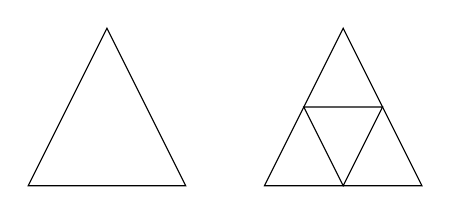
\begin{tikzpicture}
            % 三角形
            \draw (2, 1) -- (4, 1) -- (3, 3) -- cycle;
            \draw (5, 1) -- (6, 3) -- (7, 1) -- cycle;
            \draw (5.5, 2) -- (6.5, 2) -- (6, 1) -- cycle;
          \end{tikzpicture}
          \caption{全局加密一次的网格}
        \end{minipage}
        \begin{minipage}[t]{0.6\textwidth}
          \centering
          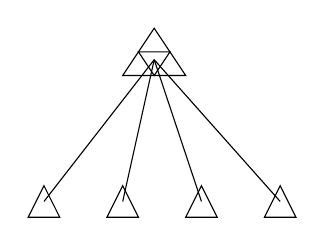
\begin{tikzpicture}
            %五个小三角形
            \draw (1.0, 0.0) -- (1.2, 0.4) -- (1.4, 0.0) -- cycle;
            \draw (2.0, 0.0) -- (2.2, 0.4) -- (2.4, 0.0) -- cycle;
            \draw (3.0, 0.0) -- (3.2, 0.4) -- (3.4, 0.0) -- cycle;
            \draw (4.0, 0.0) -- (4.2, 0.4) -- (4.4, 0.0) -- cycle;
            \draw (2.6, 2.4) -- (2.2, 1.8) -- (3.0, 1.8) -- cycle;
            \draw (2.4, 2.1) -- (2.6, 1.8) -- (2.8, 2.1) -- cycle;
            %四条线
            \draw (2.6, 2.0) -- (1.2, 0.2);
            \draw (2.6, 2.0) -- (2.2, 0.2);
            \draw (2.6, 2.0) -- (3.2, 0.2);
            \draw (2.6, 2.0) -- (4.2, 0.2);
          \end{tikzpicture}
          \caption{它的几何遗传树}
        \end{minipage}
      \caption{几何遗传树结构}
      \label{fig::hgrometrytree}
    \end{figure}


\section{快速Krylov求解}
  令$\left(\{\phi_j \}_{j = 1}^n, 0 \right)^T$ 和 $\left(0, \{\phi_j\}_{j = 1}^n\right)^T$ 是速度空间$X_h$的线性元基函数。同时,
  $\{\psi_k\}_{k = 1}^m$ 为压力空间$P_H$的线性元基函数。$t_{n + 1}$ 时刻,速度解的分量形式$\vec{u}_h^{n + 1} = (u_h^{x, n + 1},
  u_h^{y, n + 1})^T$,压力数值解为 $\vec{p}_H^{n + 1}$ at $t = t_{n + 1}$,可以写为:
  \begin{equation}
    u_h^{x, n + 1} = \sum_{j = 1}^{n_u} \alpha_j^{x, n + 1} \phi_j,
    \qquad u_h^{y, n + 1} = \sum_{j = 1}^{n_u} \alpha_j^{y, n + 1}
    \phi_j \qquad p_H^{n + 1} = \sum_{k = 1}^{n_p}\alpha_k^{p, n + 1}
    \psi_k.
    \label{eq::basis_fun}
  \end{equation}

  将(\ref{eq::basis_fun}) 带入弱形式
  (\ref{eq::NS_weak_form})中,可以得到一个鞍点问题:
  \begin{equation}
    \left[
      \begin{array}{lll}
        \frac{1}{dt} M + \nu A + N & 0 & B_x^T \\
        0 & \frac{1}{dt} M +\nu A + N  & B_y^T \\
        B_x & B_y & 0
      \end{array}
    \right]
    \left[
      \begin{array}{c}
        \alpha^{x, n + 1} \\
        \alpha^{y, n + 1} \\
        \alpha^{p, n + 1}
      \end{array}
    \right] =
    \left[
      \begin{array}{c}
        f_x \\
        f_y \\
        0
      \end{array}
    \right],
    \label{eq::linear_system}
  \end{equation}
  注意到散度矩阵 $B = [Bx, By]$ 为
  \begin{eqnarray}
    B_x := [B_x]_{kj} = -\left(\psi_k, \frac{\partial \phi_j}{\partial
        x} \right), k = 1, \cdots, n_p, j = 1, \cdots, n_u, \\
    B_y := [B_y]_{kj} = -\left(\psi_k, \frac{\partial \phi_j}{\partial
        y} \right), k = 1, \cdots, n_p, j = 1, \cdots, n_u.
  \end{eqnarray}
  因为速度单元上的基函数和压力单元上的基函数并不在同一张网格上,所以装配矩阵$B$并不是一个显然的过程。这需要根据上面提到的速度单元和压力单元间
  的$1-1$索引,我们可以仅仅只用速度和压力单元上的线性元函数来装配$B$,拼装$B^T$的过程类似。
  我们定义 $F_\nu^{n + 1} = \frac{1}{dt} M + \nu A + N$, 其中
  \begin{eqnarray}
    M := &[M]_{ij} =& \left( \phi_i, \phi_j \right),\quad  i,j = 1, \cdots,
    n_u, \\
    A := &[A]_{ij} =& \left( \nabla \phi_i, \nabla \phi_j \right), i,j =
    1, \cdots, n_u, \\
    N := &[N]_{ij} =& \left(\vec{u}_h^n, \nabla \phi_i, \phi_j \right),
    i,j = 1, \cdots, n_u.
  \end{eqnarray}

  为了高效的求解线性方程组(\ref{eq::linear_system}),我们用预处理的GMRES(generalized minimal residual algorithm)作为求解器。在\cite{elman2005finite}
  中考虑的块三角预处理$\mathcal{P}$定义如下:
  \begin{equation}
    \mathcal{P} =
    \left(
      \begin{array}{lll}
        F & 0 & B_x^T \\
        0 & F  & B_y^T \\
        0 & 0 & S
      \end{array}
    \right)
  \end{equation}
  其中 $S = B_xF^{-1}B_x^T + B_yF^{-1}B_y^T$ 是 Schur 补矩阵。预处理就是要完成近似矩阵的求逆,实施$\mathcal{P}^{-1}$的过程分为两步,
  第一步是求解schur补的系统,第二步是求解两个纯量的跟$F$有关的系统。直接求解schur补的方程组是非常耗时的,因为它系数矩阵里包含一个逆
  矩阵。所以,在实际的计算中,找到schur补的近似矩阵,然后用近似矩阵代替schur补矩阵来进行求解。\cite{elman2005finite}一文中提到PCD预
  处理可以用来作为schur补的近似。PCD矩阵定义为:
  \begin{equation}
    S_* = A_p F_p^{-1} Q_p.
    \label{eq::PCD}
  \end{equation}
  其中$A_p, F_p$ 和 $Q_p$全部定义在压力空间上。 $Q_p$ 是压力质量矩阵, $A_p$ 是压力刚度矩阵,$F_p$ 是对流扩散矩阵,它们分别定义为:
  \begin{eqnarray}
    F_p := [F_p]_{ij} = \nu (\nabla \psi_i, \nabla \psi_j) +
    (\vec{u}_h^n \cdot \nabla \psi_i, \psi_j), \quad i,j = 1, \cdots, n_p, \\
    A_p := [A_p]_{ij} = (\nabla \psi_i, \nabla \psi_j)\quad i,j = 1, \cdots,
    n_p.
    \label{eq::pcd_mat}
  \end{eqnarray}
  令
  \begin{equation}
    W_p^n := [W_p^n]_{ij} = (\vec{u}_h^n \cdot \nabla \psi_i,
    \psi_j), \quad i,j = 1, \cdots, n_p.
  \end{equation}
  那么$F_p$ 可以被重新写成:
  \begin{equation}
    F_p = \nu A_p + W_p^n.
  \end{equation}
  我们实施PCD预处理通过
  \begin{equation}
    S_*^{-1} \approx Q_p^{-1} F_p A_p^{-1}.
  \end{equation}
  精确的PCD 预处理算子定义为
  \begin{equation}
    \mathcal{M}^{-1} =
    \left(
      \begin{array}{lll}
        F^{-1} & 0 & B_x^T \\
        0 & F^{-1} & B_y^T \\
        0 & 0 &S_*^{-1}
      \end{array}
    \right)
  \end{equation}
  我们分两步解释预处理的求解过程:令$V^d = \mathcal{M}^{-1} V^s$,
  其中
  \begin{equation}
    V^d = (V_x^d, V_y^d, V_p^d)^T, V^s = (V_x^s, V_y^s, V_p^s)^T.
  \end{equation}
  第一步我们求解:
  \begin{equation}
    V_p^d = S_*^{-1} V_p^s = Q_p^{-1} F_p A_p^{-1} V_p^s.
    \label{eq::solve_schur}
  \end{equation}
  它其中包含两个possion问题的求解$Q_p^{-1}$ and $A_p^{-1}$,所以我们可以用为求解possion问题设计的多重网格求解器来实现求解。
  第二步我们再用这种多重网格求解器去求解
  \begin{equation}
    \begin{aligned}
      V_x^d = F^{-1} (V_x^s - B_x^T V_p^d), \\
      V_y^d = F^{-1} (V_y^s - B_y^T V_p^d).
    \end{aligned}
    \label{eq::solve_velocity}
  \end{equation}
  将(\ref{eq::solve_schur}) 和 (\ref{eq::solve_velocity})中的解合并在一起,就得到了要求解的 $V^d$.

  在实际的计算中,我们对矩阵$F$, $F_p$, $Q_p$, 和 $A_p$的求解,是用固定的几步代数多重网格迭代(algbraic multi-grid)来代替精确求解。这
  就是迭代的PCD方法。我们用的多重网格求解器是在AFEPack中(一个自适应有限元包),可以从\url{http://dsec.pku.edu.cn/~rli}获得。在(\cite{elman2005finite},
  第10章)中,数值算例说明了PCD预处理的高效。\cite{elman2011fast}一文将PCD预处理方法应用到bouyancy驱动流问题上。在我们的数值实验中,发现如果将
  \eqref{eq::pcd_mat}中的
  \begin{equation}
    F_p = \nu A_p + W_p^n.
  \end{equation}
  中$A_p$前面的系数去掉,会发现GMRES的迭代步数会减少。我们采用(\cite{elman2009boundary})中在Neumann边界上的处理矩阵$F_p$ 和 $A_p$的方法,来提高
  求解效率。$F_p$需要在边界$\partial \Omega = \partial \Omega_D \cup \partial \Omega_N$上满足边界条件
  \begin{equation}
    \nu \frac{\partial p_h}{\partial n} + (\vec{w}_h \cdot \vec{n})
    p_h = 0.
    \label{eq::bc_Fp}
  \end{equation}
  我们知道对于方腔流,在所有的边界上$\vec{w}_h \cdot \vec{n} = 0$,所以(\ref{eq::bc_Fp})将会退化成
  \begin{equation}
    \frac{\partial p_h}{\partial n} = 0.
  \end{equation}
  这就意味着我们在所有的边界$\partial \Omega$上,对$F_p$不采取任何操作,$A_p$采取同样的操作。
  在本文中,我们将PCD预处理方法应用到移动网格有限元方法,来高效地求解Navier-Stokes问题\eqref{eq::linear_system}。
\section{移动网格策略}
  \subsection{网格移动的流程}
     再上一章中我们详细的介绍过移动网格的策略,这一章中简要描述一下。在$t = t_{n}$时刻,我们获得了数值解 $\vec{u}_h^{(n)}, p_H^{(n)}$ 在$t_n$时刻的
     网格 $\mathcal{T}_h^n$上。我们根据\cite{di2005moving}中的方法,用保持散度为0的差值方法将$\mathcal{T}_h^n$上的数值解差值到$t_{n + 1}$时刻的网格
     $\mathcal{T}_h^{(n + 1)}$上。简单的来说,总共分为三步:
     \begin{enumerate}[step 1]
     \item 获取控制函数。 令$m = 1/G$,其中$G$是控制函数。基于涡量的控制函数
       \begin{equation}
         \centering
         G = \sqrt{1 + \alpha |\omega|^\beta}.
         \label{eq::monitor_vorticity}
       \end{equation}
       其中 $\omega = \nabla \times \vec{u}$, $\alpha, \beta$
       是两个正的常数。在本文中,$\beta = 2$有比较的效果,$\alpha$ 根据不同的问题,选取不同的值。
       problems.

     \item 获取物理网格上的移动方向。求解
       \begin{equation}
         \begin{aligned}
           \nabla_{\vec{x}}(m \nabla_{\vec{x}} \vec{\xi}) = 0, \\
           \vec{\xi}|_{\partial \Omega} = \vec{\xi}_b.
         \end{aligned}
         \label{eq::logical}
       \end{equation}
       来获得一个新的逻辑网格$\mathcal{T}_c^*$,$\mathcal{A}^*$ 作为它的节点。
       我们可以得到新的逻辑网格和初始逻辑网格$\mathcal{T}_c^0(\mbox{节点为} \mathcal{A}^0)$
       之间的误差
       \begin{equation}
         \delta \mathcal{A} = \mathcal{A}^0 - \mathcal{A}^*.
       \end{equation}
       我们可以根据$\delta \mathcal{A}$来获得物理区域的位移$\delta X_i$,通常再乘上一个正的常数$\mu$
       避免网格缠接:
       \begin{equation}
         X_i^{(n + 1)} = X_i^{(n)} + \mu \delta X_i.
       \end{equation}
     \item 保持散度为0的差值。
       在用移动网格有限元方法来求解不可压流体方程的时候,需要在数值解差值的过程中保持散度为0。在\cite{di2005moving}中,
       数值解在新网格$\mathcal{T}^{(n + 1)}$上的重新分布,是通过求解一个类似无粘的Navier-Stokes方程。
       \begin{eqnarray}
         \begin{aligned}
           \frac{\partial \vec{u}}{\partial \tau} - \nabla_{\vec{x}}\vec{u}
           \cdot \delta \vec{x} & =  - \nabla \hat{p},& \\
           \nabla_{\vec{x}}\cdot \vec{u} & =  0.&
         \end{aligned}
         \label{eq::continous_update}
       \end{eqnarray}
       其中 $\delta \vec{x} := x^{\text{old}} - x^{\text{new}}$,
       $x^{\text{old}}, x^{\text{new}}$ 是物理区域上的两组坐标。$\tau$ 是一个虚拟时间,通常取成$1.0$。因为对流速度$\delta \vec{x}$
       相对较小。这里 $\hat{p}$ 是一个临时变量,为了跟(\ref{eq::NS})中的压力变量区别开来。

       (\ref{eq::continous_update})的弱形式是: 寻找 $(\vec{u}_h, \hat{p}_H) \in X_E^h \times P^H$ 使得
       \begin{eqnarray}
         \begin{aligned}
           \left( \partial_{\tau} \vec{u}_h - \nabla_{\vec{x}}\vec{u}_h
           \cdot \delta \vec{x}, \vec{v}_h \right) & =  \left( \hat{p}_H, \nabla
           \vec{v}_h \right), \quad \forall \vec{v}_h \in X_E^h,&  \\
           \left( \nabla_{\vec{x}} \cdot \vec{u}, q_H\right) & =  0, \quad \forall
           q_H \in P^H. &
         \end{aligned}
         \label{eq::semi_discreted_update}
       \end{eqnarray}

       在本文中,我们用时间层上用显示格式离散:
       (\ref{eq::semi_discreted_update}) for time discretization:
       \begin{eqnarray}
         \begin{aligned}
           \left ( \frac{\vec{u}_{h, *}^{(n)} - \vec{u}_h^{(n)}}{\delta
               t},
           \vec{v}_h \right) + \left( \delta \vec{x} \cdot \nabla
           \vec{u}_{h}^{(n)}, \vec{v}_h \right)  & =  \left(
           \hat{p}_{H, *}^{(n)}, \nabla \vec{v}_h \right), \quad
           \forall \vec{v}_h \in X_E^h. &\\
           \left( \nabla \cdot \vec{u}_{h, *}^{n}, q_H \right) & =  0, \quad
           \forall q_H \in P^H. &
         \end{aligned}
         \label{eq::full_discreted_update}
       \end{eqnarray}
       其中$\vec{u}_h^{(n)}$ 和 $p_H^{(n)}$ 是 方程(\ref{eq::NS}) 在 $t = t_{n}$ 时刻的网格上计算的数值解。$\vec{u}_{h,*}^{(n)}$ 和 $p_{h, *}^{(n)}$
      是在新网格$\mathcal{T}^{(n + 1)}$上,$t_n$时刻的数值解,是一个中间变量。
     \end{enumerate}

   \subsection{用AMG 预处理求解(\ref{eq::full_discreted_update})}
   (\ref{eq::full_discreted_update}) 将会得到一个线性系统, 它的系数矩阵为$\mathcal{M}^p$,定义如下:
   \begin{equation}
     \mathcal{M}^p =
     \left(
       \begin{array}{lll}
         \frac{1}{\delta t} Q_p & 0 & B_x^T \\
         0 & \frac{1}{\delta t} Q_p & B_y^T \\
         B_x & B_y & 0
       \end{array}
     \right)
     \label{mat::moving}
   \end{equation}
   据我们所知,矩阵$\mathcal{M}^p$的schur补矩阵为:
   \begin{equation}
    M_S = B_x Q_p^{-1} B_x^T + B_y Q_p^{-1} B_y^T.
   \end{equation}
   根据(\cite{elman2005finite}, 第5章),对于满足LBB条件的混合元近似,当边界条件全部是封闭流体边界时,$M_S$是跟压力空间的刚度矩阵
   $A_p$谱等价的。因此我们可以用 $A_p$ 来作为schur补矩阵的近似矩阵。那么我们可以选取
   \begin{equation}
     \mathcal{K} =
     \left(
       \begin{array}{lll}
         Q_p & 0 & B_x^T \\
         0 & Q_p & B_y^T \\
         0 & 0 & M_S^*
       \end{array}
     \right)
     \label{eq::updateSolution_precond}
   \end{equation}

   来作为(\ref{mat::moving})的块预处理矩阵,其中 $M_S^* = A_p$ 或者 $M_S^* =
   \frac{1}{\nu} A_p$。我们选择不同的$M_S^*$来作为schur补矩阵的近似矩阵,
   来对比求解效率的差别。在我们的实际计算中,$\frac{1}{\nu}A_p$ 要比 $A_p$效率要高。
   对于入流/出流问题,$A_p$ 需要在Neumann边界上做出一些修改来提高计算效率。在出流边界
   $\partial \Omega_N$上,离散的压力 $p_h$ 需要满足一个齐次的Dirichlet边界条件。
   而在$\Omega_D$上,压力$p_h$要满足Neumann条件 $\frac{\partial p_h}{\partial n} = 0$,
   那就意味着我们在Dirichlet边界上,对$A_p$不采取任何操作。细节可以参考\cite{elman2009boundary}。
   注意到,一旦网格发生移动,所有的矩阵 $M, B_x^T, B_y^T, B_x, B_y, A_p$ 都需要重新构建。

   在我们的算法中,PCD预处理的GMRES作为求解线性系统(\ref{eq::linear_system})的求解器。
   我们定义GMRES收敛的停止准则为
   \begin{equation}
     ||r^{(k)}||  \leq 10^{-6} ||r^{(0)}||
   \end{equation}
   其中 $r^{(k)}$ 是线性系统(\ref{eq::linear_system})的残差,$r^{0}$ 是(\ref{eq::linear_system})的右端项的残差。
   最后,为了清楚地表述我们的算法,我们给出算法的流程图如下:

      \begin{algorithm}
        \caption{移动网格有限元方法求解Navier-Stokes}
        \begin{algorithmic}[1]
          \State 用AMG预处理来求解稳态的Stokes方程来获得初值值 $\vec{u}_h^{(0)}, p_H^{(0)}$.
          \While {$t_n < T$}
          \State 在$\triangle_p^{(n)}$上,用 $\vec{u}_h^{(n)}, p_H^{(n)}$ 计算控制函数,并且通过求解调和映射(\ref{eq::logical})来获得
                 新的逻辑网格$\vec{\xi}^*$。 \label{state::monitor}
          \State 判断 如果 $\vec{\xi}^* - \vec{\xi}^{(0)}$ 的 $L_2$ 范数是不是比容忍量小。若是,则迭代结束,否则
                 继续 \ref{state::start} - \ref{state::end}。
          \State 用$\vec{\xi}^* - \vec{\xi}^{(0)}$之间的误差来计算压力网格$\triangle_p^{(n)}$在物理区域上的移动量$\delta \vec{x}$。
                 \label{state::start}
          \State 在速度网格 $\triangle_v^{(n)}$ 上,用AMG预处理方法求解方程 (\ref{eq::full_discreted_update}) 来获取中间变量
                 $\vec{u}_{h, *}^{(n)}, p_{H, *}^{(n)}$。
          \State 更新压力网格 $\triangle_p^{(n)}$ 到 $\triangle_p^{(n +
                 1)}$ 并且利用几何遗传树结构来同步 $\triangle_v^{(n)}$ 到
                 $\triangle_v^{(n + 1)}$。
          \State 回到 \ref{state::monitor}。 \label{state::end}

          \State 用AMG预处理方法来求解 Navier-Stokes 问题 (\ref{eq::linear_system}),从而获得新网格$\triangle_v^{(n + 1)}$ 和 $\triangle_p^{(n
                 + 1)}$ 上的数值解 $\vec{u}_h^{(n + 1)}, p_H^{(n + 1)}$。
          \EndWhile
        \end{algorithmic}
        \label{alg::solve}
      \end{algorithm}


% ----------------------------------------------------------------------------------------
%	SECTION 6
% ----------------------------------------------------------------------------------------
\section{数值算例}
      我们用三个数值算例来展示我们的方法。在实际的计算过程中,我们采用稳态的Stokes方程的解作为Navier-Stokes方程的初始值,
      边界条件设置跟Navier-Stokes方程一致。在我们的算法中,初始的物理区域和逻辑区域是一致的。网格的移动效果以及数值解在
      下面展示出来。我们的代码是基于有限元包AFEPack。

     \subsection{方腔驱动流}
       我们考虑经典算例:正则化的方腔流。我们的计算区域是$\Omega = [-1, 1] \times [-1, 1]$,粘性系数是$\nu = 0.001$。Dirichlet
       边界条件设置在所有的边界$\partial \Omega$上。在顶部边上,速度$\vec{u} = (1 - x^4, 0)^T$,无滑移条件设置在$\partial \Omega$
       的其它部分。

       在我们的移动策略中,我们选取涡量(\ref{eq::monitor_vorticity})为控制函数。参数取成$\alpha = 0.5, \beta = 2.0$时网格移动效果
       表现好。在图\ref{fig::cavity_flow_mesh}中展示的是发展到稳态的移动网格以及涡量的等高线。我们可以看出网格集中在顶部边和右边边界
       ,这些地方都是涡量比较大的地方。速度的流速线如图\ref{fig::cavity_flow_streamline}。

       从表\ref{tab::GMRES_steps_initial}中,我们得知在PCD预处理中,选取$F_p = A_p + W_p^n$ 比 $F_p = \nu A_p + W_p^n$ 需要的迭代步数
       要少很多。在每个时间步,求解线性方程组的(\ref{eq::linear_system})的GMRES迭代步数如图\ref{fig::cavity_GMRES_steps}。它需要$12-24$
       步迭代收敛,当流体趋于稳定的时候,迭代次数在$15-16$步。


       \begin{figure}[!htbp]
         \begin{center}
             \includegraphics[width = 0.43\textwidth, angle = -90]{picture/second/cavity_flow_data/moving_mesh.eps}
             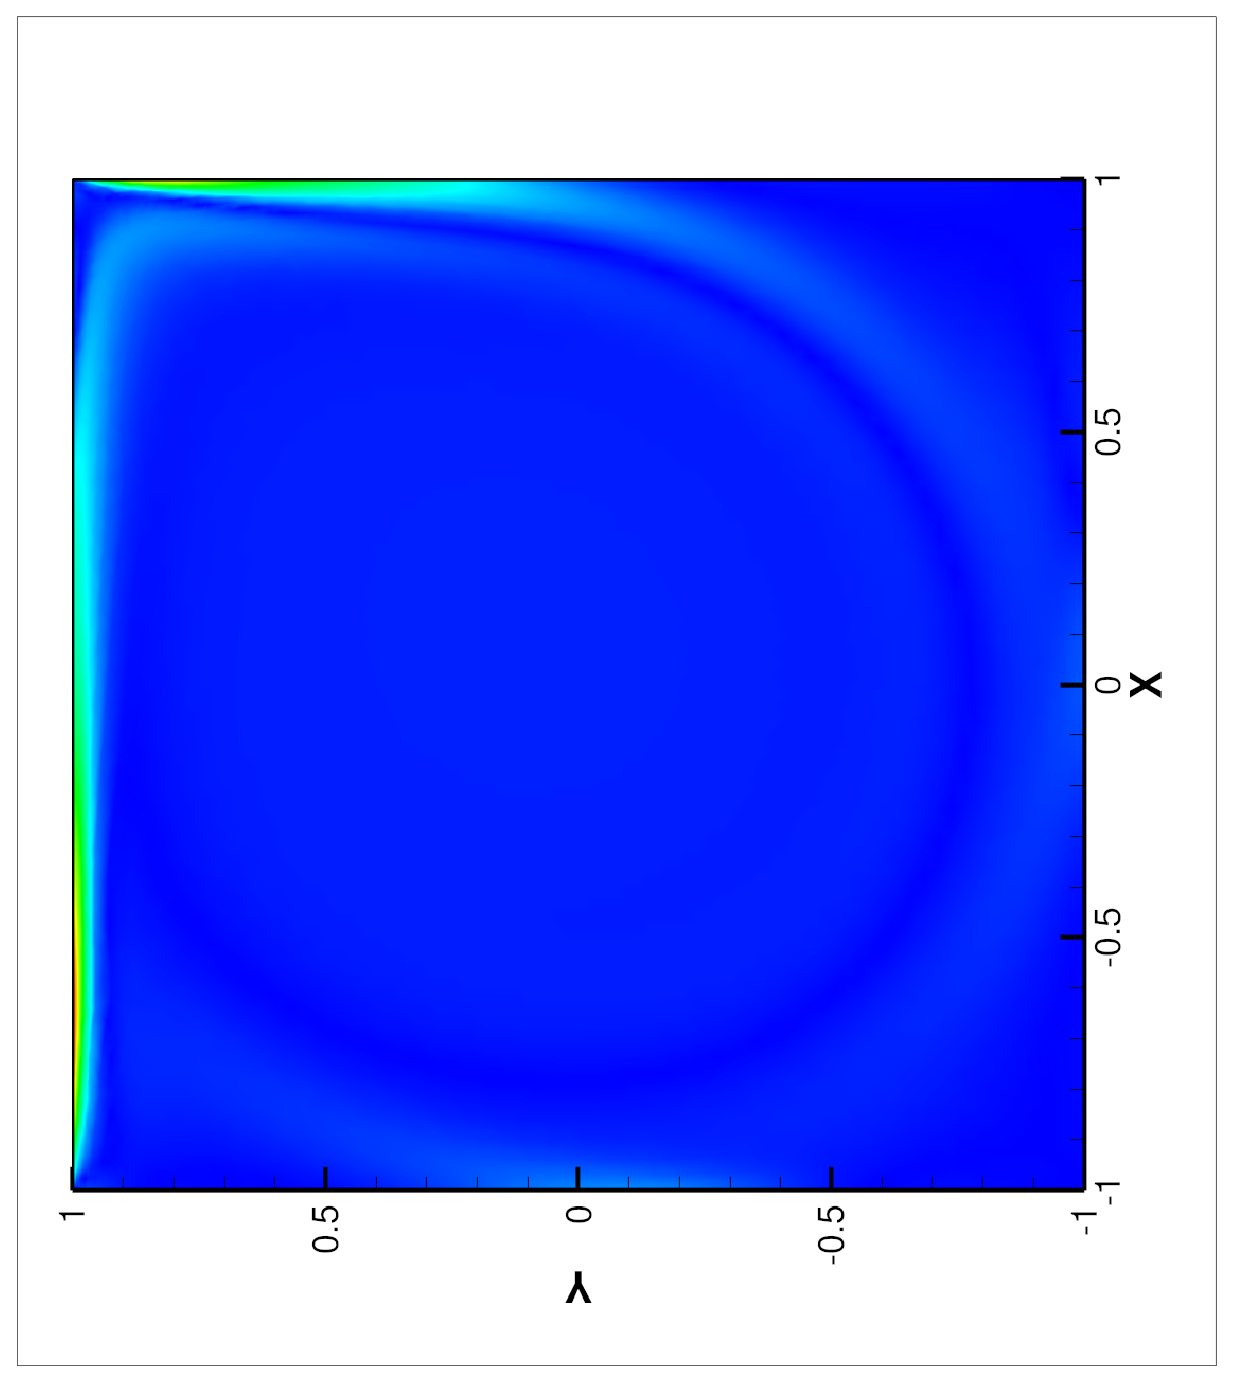
\includegraphics[width = 0.43\textwidth, angle = -90]{picture/second/cavity_flow_data/vortex.eps}
        \end{center}
        \caption{\small Cavity flow, left: mesh, right: vorticity
          contour, pressure mesh $40 \times 40$, $\nu = 0.001$.}
        \label{fig::cavity_flow_mesh}
       \end{figure}

       \begin{figure}[!htbp]
         \begin{center}
             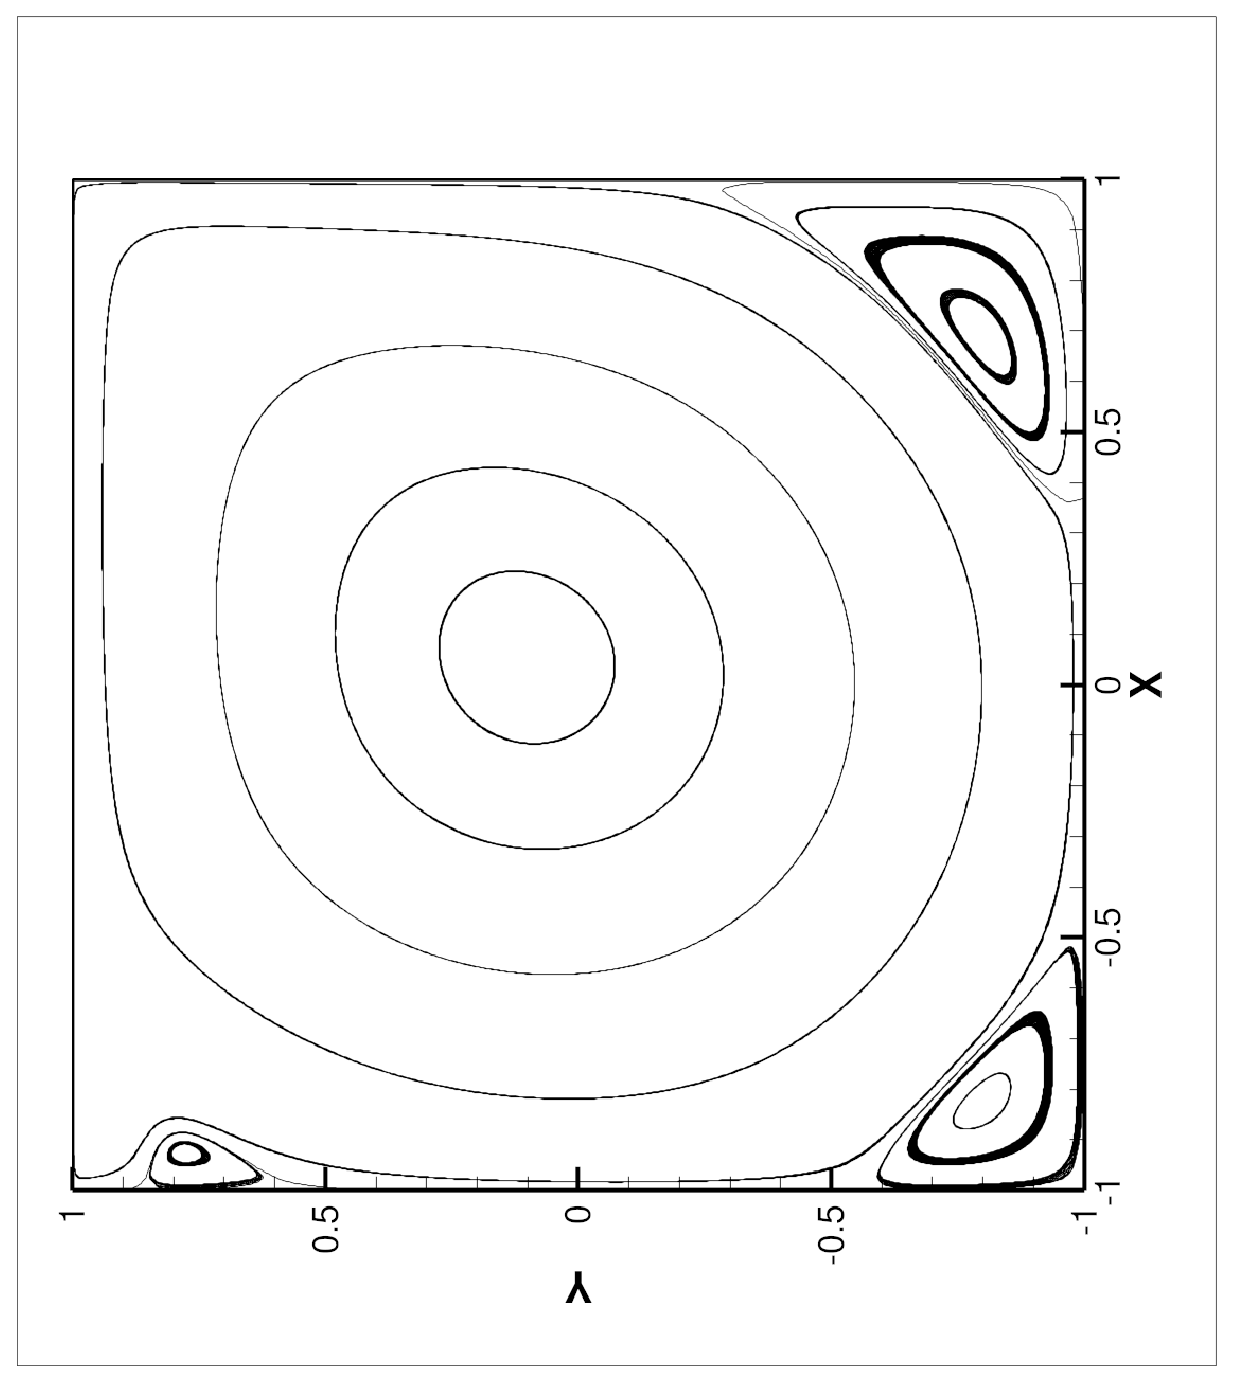
\includegraphics[width = 0.43\textwidth, angle = -90]{picture/second/cavity_flow_data/streamline.eps}
        \end{center}
        \caption{\small Cavity flow: velocity streamline, pressure
          mesh $40 \times 40$, $\nu = 0.001$.}
        \label{fig::cavity_flow_streamline}
       \end{figure}

       \begin{figure}[!htbp]
         \begin{center}
             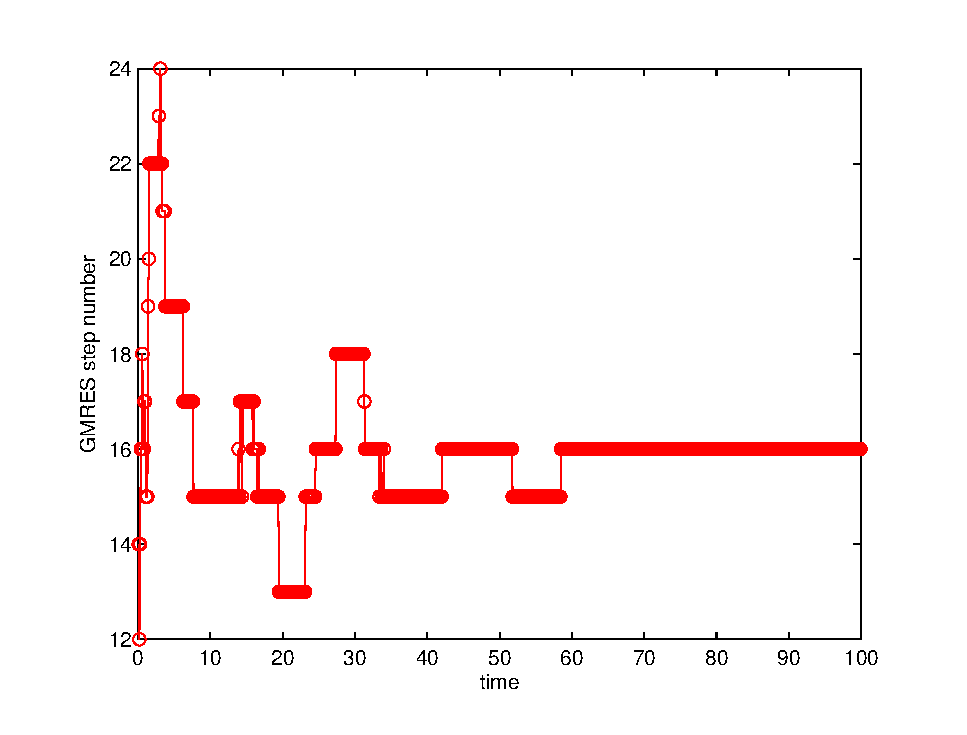
\includegraphics[width = 0.55\textwidth, angle = 0]{picture/second/cavity_flow_data/NS_iterate_steps.eps}
        \end{center}
        \caption{\small Cavity flow: GMRES step counts of solving
          (\ref{eq::linear_system}) with modified PCD preconditon,
          pressure mesh $40 \times 40$, $\nu = 0.001$.}
        \label{fig::cavity_GMRES_steps}
       \end{figure}

       \begin{table}[!htbp]
         \centering
         \begin{tabular}{cccc}
           \hline
           \multirow{2}{*}{pressure mesh}    & \multirow{2}{*}{time
             step} & \multicolumn{2}{c}{GMRES step number} \\
           \cline{3-4}
            &               & $F_p = \nu A_p + W_p^n$ & $F_p = A_p + W_p^n$ \\ \hline
           $20 \times 20$   &   $0.00656$         &      $41$           &     $8$
           \\ \hline
           $40 \times 40$   &   $0.00312$         &      $43$           &     $12$
           \\ \hline
           $80 \times 80$   &   $0.00153$   &      $48$    &     $18$
           \\ \hline
         \end{tabular}
         \caption{Cavity flow: GMRES step number of solving linear system
           (\ref{eq::linear_system}) with different $F_p$ in PCD
           preconditioning at first time step, $\nu = 0.001$.}
         \label{tab::GMRES_steps_initial}
       \end{table}
   \subsection{Backward step flow}

      这个算例模拟的是流体经过一个向后的台阶。管道的长度是$l = 5$,在入流边界$x = -1, y \in (0, -1)$设置的是Poiseuille流条件
      $\vec{u} = (1 - y^2, 0)^T$。在管道的顶端和底端设置的无滑移边界条件$\vec{u} = (0, 0)^T$,自然条件设置在出流边界$x = 5, y \in (-1, 1)$
      上。我们选取粘性系数为$\nu = 0.02$,那么当$t \rightarrow \infty$时,流体趋向于稳态。


      我们选取(\ref{eq::monitor_vorticity})为控制函数,控制函数中的参数是$\alpha = 2.0, \beta = 2.0$。我们知道奇异性将会出现在流体扩展的拐角
      处,因此这里需要更多的网格。在图 \ref{fig::step_flow_mesh_streamline}中,网格集中在凹进去的拐角处,这跟我们的设想一致。

      要满足CFL条件,我们的计算时间步长在$0.008$左右。求解 (\ref{eq::linear_system}) 和 (\ref{eq::full_discreted_update})的GMRES迭代步数在图
      \ref{fig::GMRES_steps_total} 中给出。从中可以发现求解 (\ref{eq::linear_system}) 需要少于$21$步迭代就能收敛。

      \begin{figure}[!htbp]
        \centering
        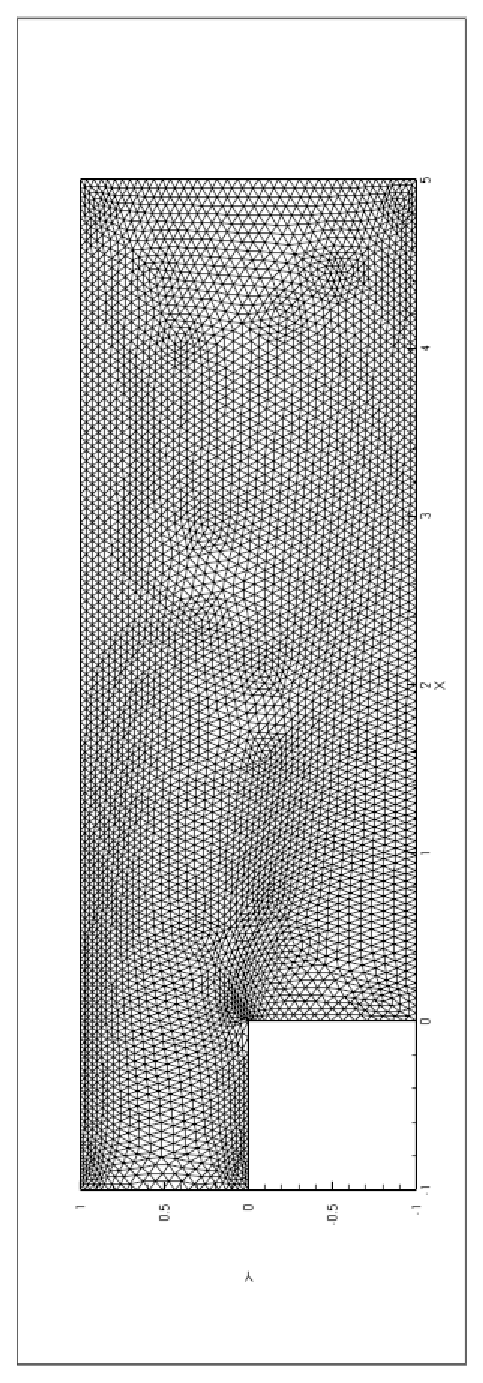
\includegraphics[width = 0.3\textwidth, angle =
        -90]{picture/second/L_shaped_flow_data/mesh.eps}
        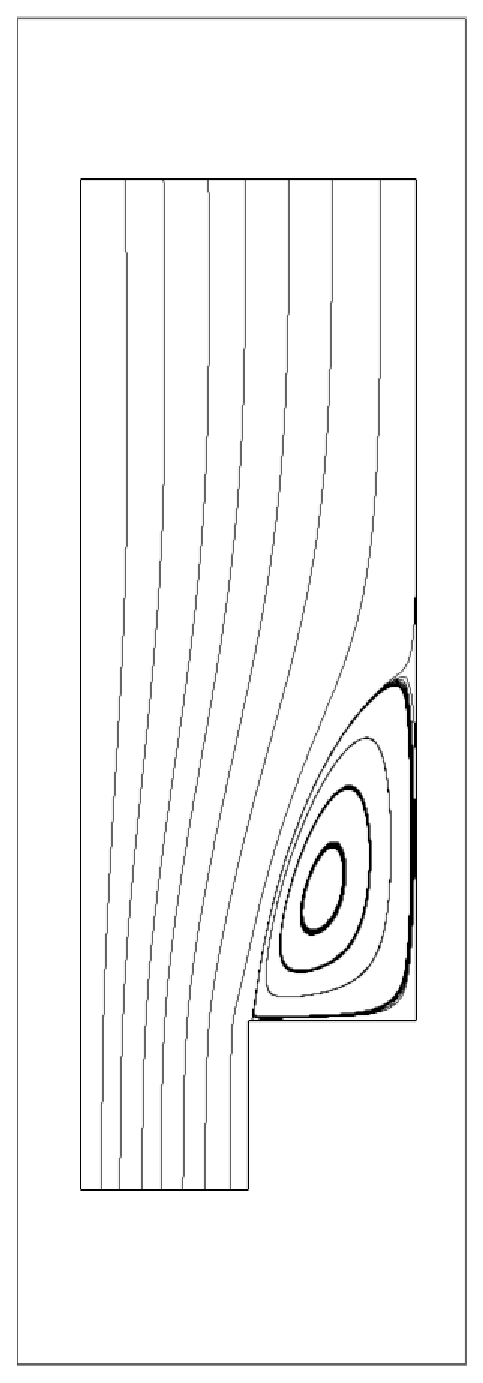
\includegraphics[width = 0.3\textwidth, angle =
        -90]{picture/second/L_shaped_flow_data/streamline.eps}
        \caption{\small Top: moving mesh, bottom: velocity streamline
          in step flow at $t = 100s$, viscosity $\nu = 0.02$.}
        \label{fig::step_flow_mesh_streamline}
      \end{figure}

      \begin{figure}[!htbp]
        \centering
        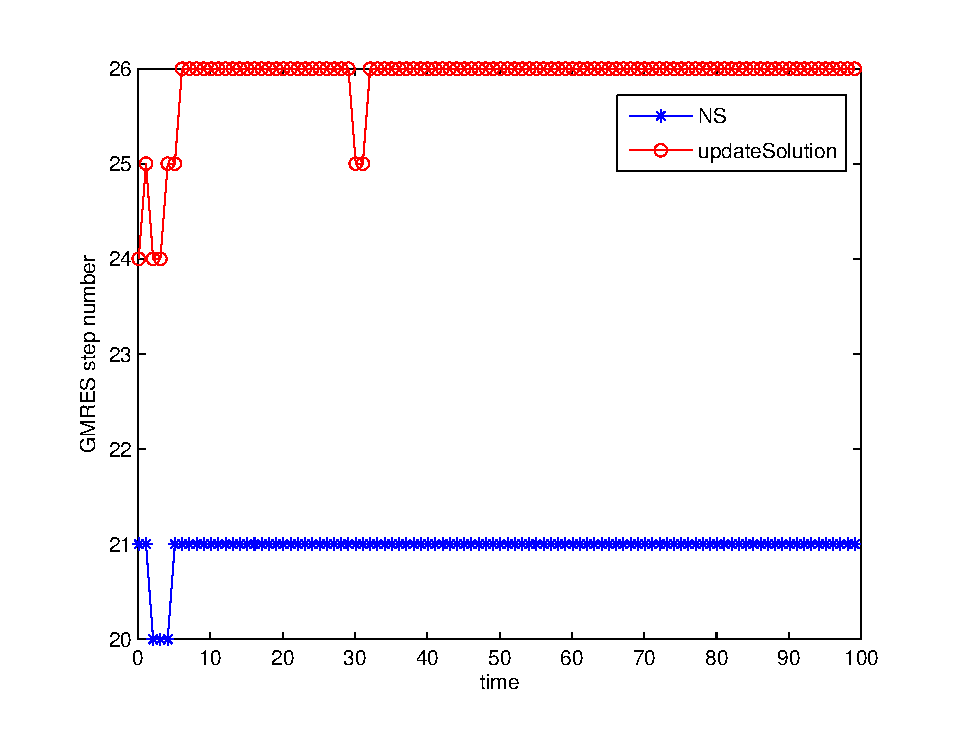
\includegraphics[width = 0.55\textwidth, angle = 0]{picture/second/L_shaped_flow_data/iterate_steps.eps}
        \caption{\small Step flow: GMRES iteration counts via time, $\nu = 0.02$}
        \label{fig::GMRES_steps_total}
      \end{figure}

   \subsection{Flow over cylinder}

      这个算例模拟的是流体在长方形的管道流中,流过一个圆形的障碍物。这个问题在\cite{cao1999anr}中考虑过,是以流函数形式计算的。
      圆形障碍的圆心是$(0, 0)$,半径是$r = 0.3$,雷诺数是$Re = 600$,计算区域是 $\Omega = [-1, 5] \times [-1, 1]$。在入流边界
      $x = -1$,设置具有poiseuille性质的边界条件 $\vec{u} = (1 - y^2, 0)^T$。在管道的上边界和下边界,设定条件$\vec{u} = (0, 0)^T$。
      自然条件设置在出流边界 $x = 5$ 上。

      在我们的移动策略中,用户可以设置控制函数 (\ref{eq::monitor_vorticity}) 的参数$\alpha$ 和 $\beta$。$\alpha$ 的值越大,
      网格聚集的程度就越大。从图 \ref{fig::cylinder_GMRES_steps}中,我们可以看出 $\alpha = 5, \beta = 2$ 时GMRES的迭代步数
      要比 $\alpha = 1, \beta = 2$ 时的迭代次数多。当我们选择不同的PCD不同的$F_p$,GMRES迭代次数的比较在图 \ref{fig::cylinder_GMRES_steps_comparation}中给出。我们发现选择 $F_p = A + W_p^n$ 的计算效率要高于 $F_p = \nu A + W_p^n$。

      在图 \ref{fig::cylinder_mesh_2s}中,展示了 $t = 2s$ 时的网格移动效果。可以发现,网格明显的聚集在圆形障碍物的周围。据我们所知,
      当选取适当的雷诺数时,会出现涡街现象,参考\cite{milton1982album}一文,正如图 Figure \ref{fig::cylinder_mesh_40s}所展示的。

      \begin{figure}[!htbp]
        \begin{center}
          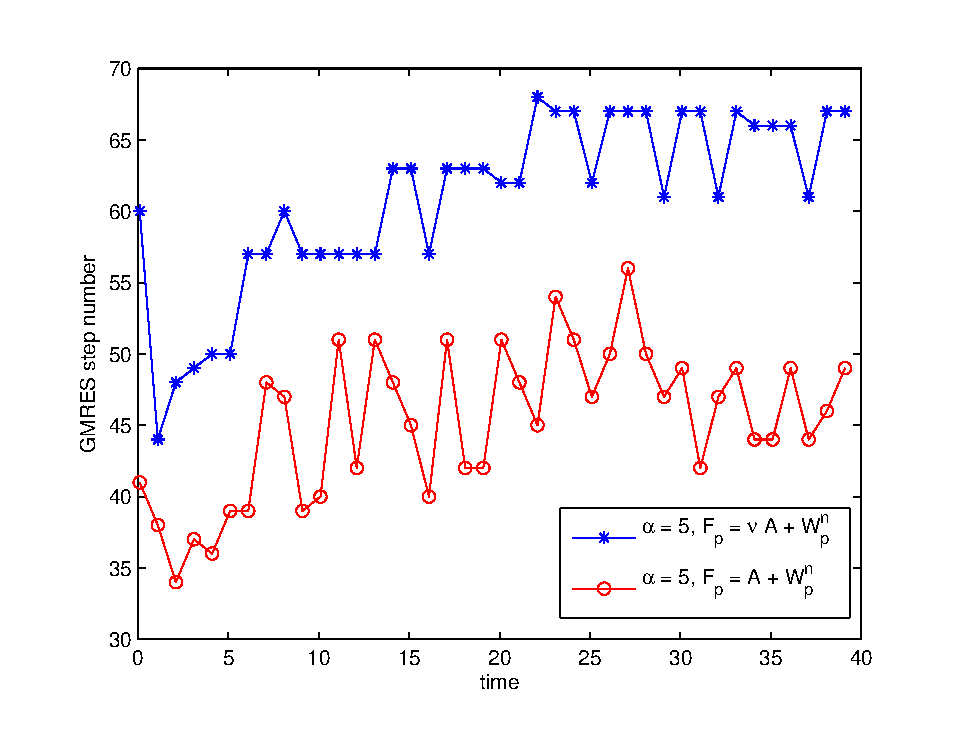
\includegraphics[width = 0.55\textwidth]{picture/second/obstacle_flow_data/comparation_NS_iterate_step.eps}
        \end{center}
        \caption{\small Flow over cylinder: GMRES iteration counts of
                 solving(\ref{eq::linear_system}) with different $F_p$ in
                 preconditioning, $\alpha = 5.0, \nu = 1/300$.}
        \label{fig::cylinder_GMRES_steps_comparation}
      \end{figure}

      \begin{figure}[!htbp]
        \begin{center}
          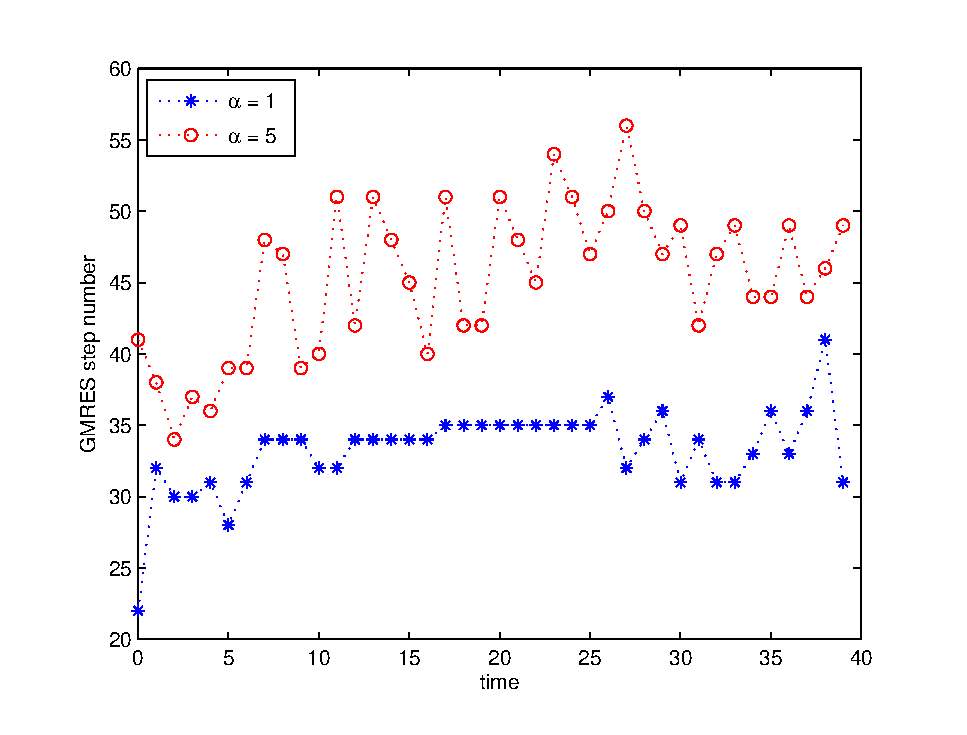
\includegraphics[width = 0.45\textwidth]{picture/second/obstacle_flow_data/NS_iterate_steps.eps}
          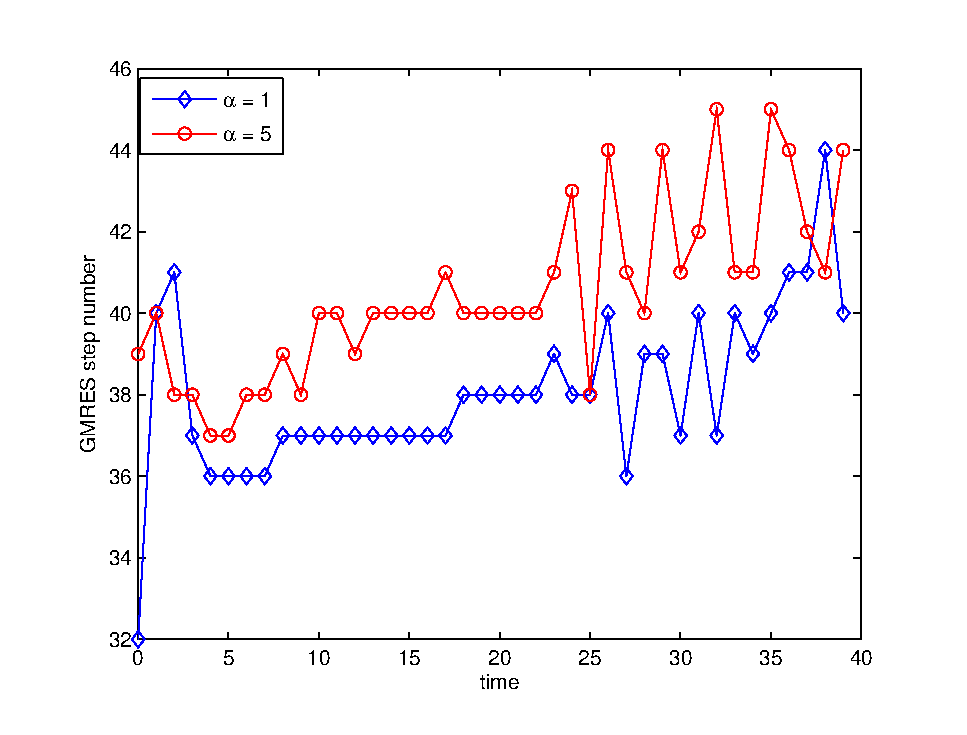
\includegraphics[width = 0.45\textwidth]{picture/second/obstacle_flow_data/moving_iterate_steps.eps}
        \end{center}
        \caption{\small Flow over cylinder, left: GMRES iteration counts of
          solving (\ref{eq::linear_system}), right: GMRES iteration
          counts of solving (\ref{eq::full_discreted_update}), $\nu =
          1/300$.}
        \label{fig::cylinder_GMRES_steps}
      \end{figure}


      \begin{figure}[!htbp]
        \centering
        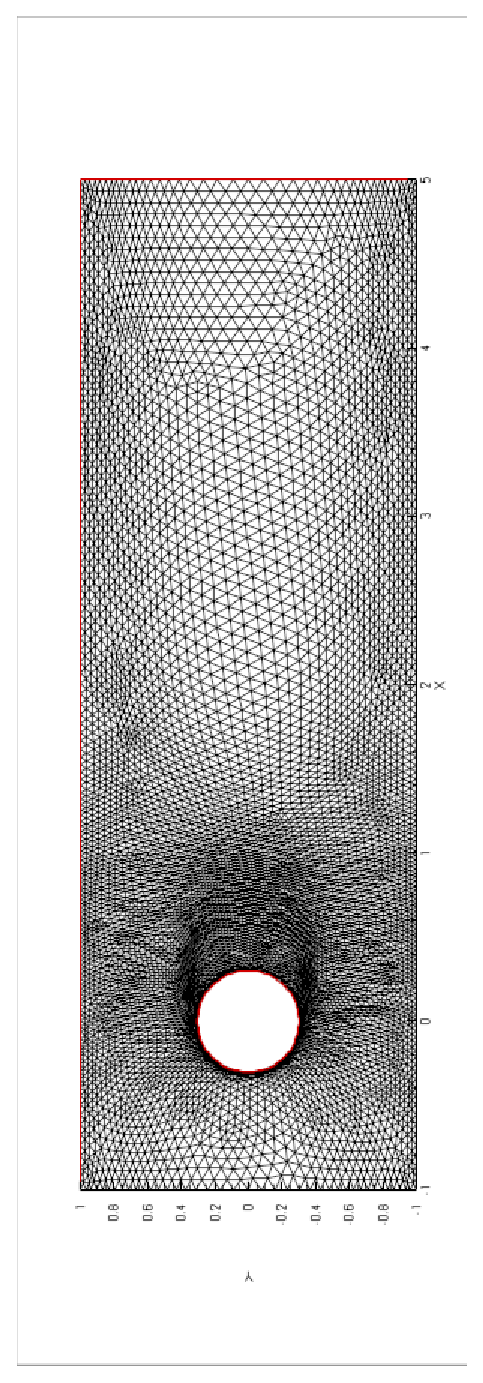
\includegraphics[width = 0.3\textwidth, angle = -90]{picture/second/obstacle_flow_data/mesh_t_2s.eps}
        \caption{\small Flow over cylinder: moving mesh at $t = 2s$,
          viscosity $\nu = 1/300$}
        \label{fig::cylinder_mesh_2s}
      \end{figure}

      \begin{figure}[!htbp]
        \centering
        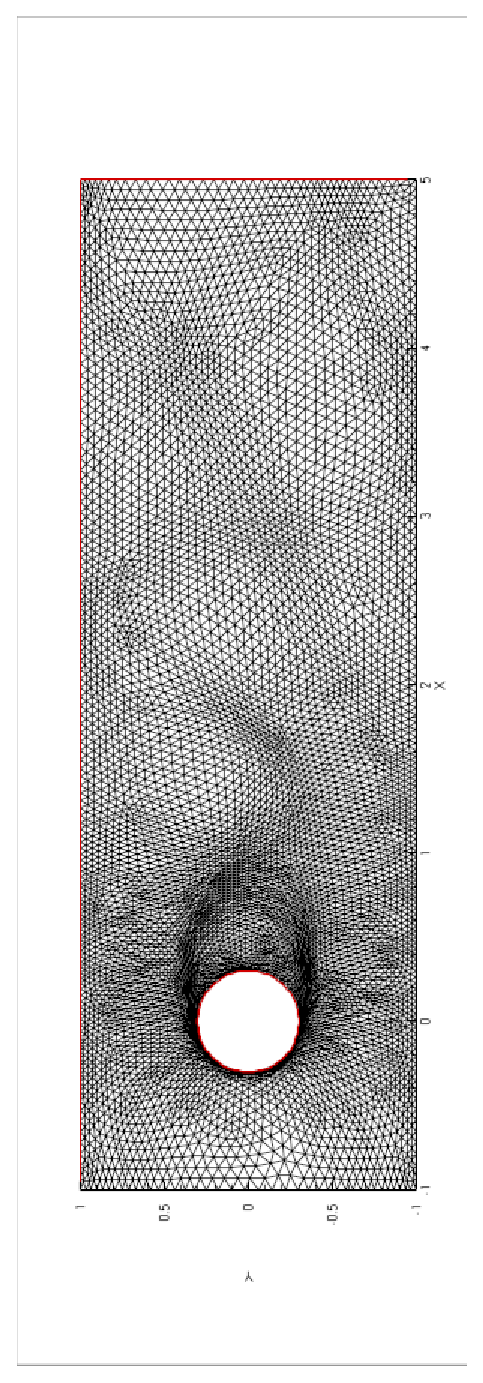
\includegraphics[width = 0.3\textwidth, angle = -90]{picture/second/obstacle_flow_data/mesh_t_40s.eps}
        \caption{\small Flow over cylinder: moving mesh at $t = 40s$,
          viscosity $\nu = 1/300$.}
        \label{fig::cylinder_mesh_40s}
      \end{figure}





  %=== 参考文献 ===%
  % 使用 BibTeX
  \bibliography{references/mathpaper, references/MathBook}
  %GATHER{references/LingBib.bib}
  % 不使用BibTex
  %%%---------------------------------------------------------------------------%%
%%------------------------------ ����� -----------------------------------%%
%%---------------------------------------------------------------------------%%


\begin{thebibliography}{30}

\bibitem{Candela1990} V. Candela and A. Marquina,
Recurrence Relations for Rational Cubic Methods I: The Halley
Method, Computing, 44 (1990) 169-184.

\bibitem{Deuflhard1979} Peter Deuflhard and G. Heindl, Affine
Invariant Convergence Theorems for Newton's Method and Extensions to
Related Methods, SIAM J. Numer. Anal., 16 (1979) 1-10.

\bibitem{Deuflhard2004} Peter Deuflhard, Newton Methods for
Nonlinear Problems: Affine Invariance and Adaptive Algorithms,
Springer-Verlag, Berlin Heidelberg, 2004.

\bibitem{Deuflhard1992} Peter Deuflhard and Florian A. Potra,
Asymptotic Mesh Independence of Newton-Galerkin Methods via a
Refined Mysovskii Theorem, SIAM J. Numer. Anal., 29 (1992)
1395-1412.

\bibitem{Ezquerro2005} J.A. Ezquerro and M.A. Hern\'{a}ndez, On
the R-Order of the Hally Method, J. Math. Anal. Appl., 303 (2005)
591-601.

\bibitem{Gutierrez1997} J.M. Guti\'{e}rrez and
M.A. Hern\'{a}ndez, Third-order Iterative Methods for Operators with
Bounded Second Derivative, J. Comput. Appl. Math., 82 (1997)
171-183.

\bibitem{Gutierrez2000} J.M. Guti\'{e}rrez and
M.A. Hern\'{a}ndez, Newton's Method under Weak Kantorovich
Conditions, IMA J. Numer. Anal., 20 (2000) 521-532.

\bibitem{Kantorvich1982} L.V. Kantorvich and G.P. Akilov,
Functional Analysis, Pergamon Press, Oxford, 1982.

\bibitem{Melman1997} A. Melman, Geometry and Convergence of Euler's
and Halley's Methods, SIAM Rev., 39 (1997) 728-735.

\bibitem{Wang2000} Xinghua Wang, Convergence of Newton's Method and
Uniqueness of the Solution of Equations in Banach Space, IMA J.
Numer. Anal., 20 (2000) 123-134.

\bibitem{WangLiLai2002} Xinghua Wang, Chong Li and Mingjun Lai, A
Unified Convergence Theory for Newton-Type Methods for Zeros of
Nonlinear Operators in Banach Spances, BIT, 42 (2002) 206-213.

\bibitem{Weiser2005} Martin Weiser, Anton Schiela and Peter
Deuflhard, Asymptotic Mesh Independence of Newton's Method
Revisited, SIAM J. Numer. Anal., 42 (2005) 1830-1845.

\bibitem{XuLi2007} Xiubin Xu and Chong Li, Convergence of
Newton's Method for Systems of Equations with Constant Rank
Derivatives, J. Comput. Math., 25 (2007) 705-718.

\bibitem{XuLi2008} Xiubin Xu and Chong Li, Convergence Criterion
of Newton's Method for Singular Systems with Constant Rank
Derivatives, J. Math. Anal. Appl., 345 (2008) 689-701.

\bibitem{Yao1999} Qingchuan Yao, On Halley Iteration, Numer. Math.,
81 (1999) 647-677.

\bibitem{YeLi2006} Xintao Ye, Chong Li, Convergence of the
Family of the Deformed Euler-Hally Iterations under the H\"{o}lder
Condition of the Second Derivative, J. Comput. Appl. Math., 194
(2006) 294-308.

\end{thebibliography}



  %=== 附录 ===%
%  \appendix
%  \include{Chapters/chaptersrequires}


%%===========================================================================%%
%%========================= 附件部分 ========================================%%
%%===========================================================================%%

%它不再对章进行自动编号,但不改变页码数字格式,不重设页码计数器
\backmatter


  %=== 发表文章目录 ===%
  %%---------------------------------------------------------------------------%%
%%----------------------------- �о��ɹ� ------------------------------------%%
%%---------------------------------------------------------------------------%%
\begin{publications}{20}

\item
An analysis on efficiency of Euler's method for computing the matrix
pth root, 2013, in preparation.

\item
A note on Newton's method and Halley's method for computing the
matrix pth root, 2013, in preparation.

\item
On the semilocal convergence behavior for Halley's method, Comput.
Optim. Appl., 2014.

\item
A globally convergent inexact Newton-like Cayley transform method
for inverse eigenvalue problems, J. Appl. Math., 2013.

\item
Convergence behavior for Newton-Steffensen's method under
gamma-condition of second derivative, Abstr. Appl. Anal., 2013.

\end{publications}


    %=== 致谢 ===%
  %%---------------------------------------------------------------------------%%
%%------------------------------- ��л --------------------------------------%%
%%---------------------------------------------------------------------------%%




\begin{thanks}
�������ڻ�������ڵ�Ϥ��ָ������ɵ�.
�dz���л����ʦ����������ѡ���о���������,
ʹ���ܹ��л�����һ���dz�����˼����������һЩ�о�����.
����ʦԨ����֪ʶ���Ͻ�����ѧ̬��ʹ�������dz,
ͬʱ��˼�롢�����϶���Ҳ�ܹ��ĺ��չ�, ֵ�˱�ҵ֮��,
���������Գ�ߵľ���ͳ�ֿ��л�⣮

��˻���, �һ�Ҫ��л�ҵ�ͬ��ʦ�ֽ������,
�����������۰༰ʵ������Ľ���ʹ�������dz, �����ǣ�
�����������ۡ���ά����С�ࡢ����ϡ�֣诡������졢��������������������
���񷼡�֣�ϡ������M��DZ��ӡ�����ࡢ����.

��л���й����ҡ�֧���ҡ������ҵ����˺������ǣ�
\end{thanks}


  %=== 学位论文独创性声明和学位论文使用授权声明 ===%
  %%---------------------------------------------------------------------------%%
%%------------------------------- ���� --------------------------------------%%
%%---------------------------------------------------------------------------%%

\
\newpage

\begin{minipage}{15cm}
\begin{OriginalityStatements}
\

\setlength{\parindent}{2em}
�����������ʽ���ѧλ�������Ҹ����ڵ�ʦָ����
���е��о�������ȡ�õ��о��ɹ���
�����г����ر���Ա�ע����л�ĵط��⣬
�����������˻����������Ѿ�������׫д�����о��ɹ���
����ͬ־�Ա��о��������������Ĺ��׾�������������
����ȷ����������ʾ��л�⣮
������ȫ��ʶ���������ķ��ɽ���ɱ��˳е���
\newline
\newline

\CASTspace ����ǩ����\CASTspace \CASTspace \CASTspace \CASTspace
\CASTspace ���ڣ�\CASTspace \CASTspace �� \CASTspace �� \CASTspace
��
\\[3cm]
\end{OriginalityStatements}



\begin{LicenseStatements}
\

\setlength{\parindent}{2em}
������ȫ�˽��㽭��ѧ�йر�����ʹ��ѧλ���ĵĹ涨��
����ѧУ��Ȩ������������йػ��ػ�����ͽ����ĵĸ�ӡ���͵����ĵ���
�������ı����ĺͽ��ģ����Բ���Ӱӡ����ӡ��ɨ����ֶα��桢���ѧλ���ģ�
ͬ���㽭��ѧ�����ò�ͬ��ʽ�ڲ�ͬý���Ϸ������������ĵ�ȫ���򲿷����ݣ�

���ܵ�ѧλ�����ڽ��ܺ����ش�Э�飮
\newline
\newline

\noindent ����ǩ����\CASTspace \CASTspace \CASTspace
��ʦǩ����\CASTspace \CASTspace \CASTspace ���ڣ�\CASTspace
\CASTspace �� \CASTspace �� \CASTspace ��

\end{LicenseStatements}
\end{minipage}



\end{document}
